\pdfoutput=1

\documentclass[11pt]{article}
\usepackage[review]{acl}

\usepackage{algorithmic}
\usepackage{algorithm}
\usepackage{array}
\usepackage{amsmath}
\usepackage{amsfonts}
\usepackage{amssymb}
\usepackage{amsthm}
\usepackage{balance}
\usepackage{booktabs}
\usepackage[justification=centering]{caption}
\usepackage{cleveref}
\usepackage{comment}
\usepackage{enumitem}
\usepackage{epsfig}
\usepackage{fancyhdr}
\usepackage[T1]{fontenc}
\usepackage{geometry}
\usepackage{graphicx}
\usepackage{inconsolata}
\usepackage[utf8]{inputenc}
\usepackage{interval}
\usepackage{microtype}
\usepackage{multicol}
\usepackage{multirow}
\usepackage{rotating}
\usepackage{setspace}
\usepackage{subfigure}
\usepackage{tabularx}
\usepackage{tikz}
\usepackage{url}
\usepackage{verbatim}
\usepackage{xcolor}
\usepackage{xstring}

\usepackage[true]{anonymous-acm}

\title{LLM Output Compliance with Handcrafted Linguistic Features --- An Experiment}
\authoranon{
\author{Andrei Olar\\
Universitatea Babeș-Bolyai, Cluj-Napoca, România\\
\texttt{andrei.olar@ubbcluj.ro}\\}
}

\begin{document}
\maketitle
\begin{abstract}
    Large language models are sought for solving an increasing number of
    increasingly diverse tasks. Perhaps naturally one such task is text style
    transfer: the task of changing the style of a text while preserving its
    meaning. Besides the natural approach of fine-tuning a large language model,
    a simpler and cheaper alternative should also be investigated: using
    handcrafted language features to direct the large language model.
\end{abstract}


\section{Introduction}\label{introduction}

\textbf{Large language models (LLMs)} have are a commonplace research topic
today.
Because language models such as BERT~\cite{devlin2018bert} or
GPT~\cite{gpt-2018,gpt2-2019,gpt3-2020} constantly advance the state of the art
on many natural language processing tasks, it has become natural to want to
evaluate the performance of these generalist models on ever more specialized
tasks.
We know from multiple surveys~\cite{minaee2024llmsurvey,zhao2023survey} and
benchmarks~\cite{papcode2024hellaswag,chiang2024chatbot} that large language
models (especially the more popular ones) are good at following instructions.
We can also intuit that training LLMs on diverse data (for instance the
Pile~\cite{gao2020pile}) uniquely qualifies them to produce text in a wide
variety of styles.

\textbf{Text style transfer (TST)} is defined as the ``task of transforming the
stylistic manner in which a sentence is written, while preserving the meaning of
the original sentence''~\cite{tst-review-2021}.
This definition can be extended to entire articles or corpuses of text because
these are also the object of linguistic style and
stylistics~\cite{lugea2023stylistics}.
The task of transfering text style is an old preocupation for the natural
language processing and computational linguistics communities which has picked
up interest again in the context of the advancements in the field of deep
learning and particularly since the inception of the transformer architecture.

\textbf{Handcrafted linguistic features (HLFs)} are single numerical values
produced by a uniquely identifiable method on any natural
language~\cite{lftk-2023}.
More often than not, these values are easy to compute while the methods used for
obtaining them are usually idempotent.
This makes them very attractive because of the dual purpose that they can serve.
On the one hand, they can be used to instruct the generation of text (``write
no more than 10 sentences'') while on the other they can be used to analyse text
and, therefore, verify generated text.

Some HLFs statistically describe text in terms of its basic syntactical and
morphological components.
Knowing this we could follow Noam Chomsky's ideas~\cite{chomsky2002syntactic}
which imply that the style of a text is influenced by its underlying syntactic
structures.
Traditionally, linguistic style was thought to be the result of morphological
and syntactic arrangements~\cite{lugea2023stylistics}.
More recent schools of thought on linguistic style find semantics and pragmatics
to be inextricably linked to author style~\cite{verma2019lexical}, but argue
that a great deal can still be inferred from lexicon, syntax and a `surface'
level which contains basic HLFs such as the number of words in a sentence.

For example, a high number of exclamations in a text is often a revealing
signal of an inflamatory news writing style, of spam or of alert narration or
dialogue.
Similar observations have been made about other characteristics of written text
that might be computed as HLFs~\cite{hovy1987generating,lugea2023stylistics}.
Combining multiple HLFs that are revelatory of linguistic style could provide us
with an easily interpretable and verifiable stylistic profile.

These apparently disparate strands of thought lead us to the two research
questions we'd like to answer in this paper.

Firstly, \textbf{is it possible to influence an LLM's writing style by
    instructing it to generate text that complies to certain HLFs}?
This problem of controlled text generation has implications for text style
transfer and authorship verification.
Answering this question might point out cheaper, less intrusive and more user
friendly solutions than fine tuning large language models for these tasks.
Fine tuning LLMs also incurs some loss of generality~\cite{yang2024unveiling},
going directly against the purpose of having a generic language model.

Secondly, we ask \textbf{if it's possible to quantify how closely an LLM is able
    to follow prompts concerning the compliance of the generated text to HLFs?}
The answer to this question could hint at a relatively simple and accurate way
of evaluating the quality of (partial) text style transfer using a large
language model.

\section{Related Work}\label{related}

There is abundent literature on the topic of text style transfer.
Reviews and surveys~\cite{tst-review-2021,tst-survey-2022} were helpful for
informing our selection of HLFs.
Studies on attaining fine-grained text style transfer using language models
have served as inspiration for writing this paper~\cite{lyu-etal-2023-fine}.
We should note though that we are not attempting to transfer text style, but
merely to instruct an LLM to follow instructions based on HLFs.

Linguistic style, then, is the sum of identifiable language choices manifest in
a text made from the language system by the text
producer~\cite{lugea2023stylistics}.
Another way to think about it is that style is the form used for delivering
meaning~\cite{tst_sigkdd_review_2022}.
The ample literature on the subject seems to agree that style depends on context
and author choice vis-a-vis a communication
goal~\cite{mcdonald1985computational,hovy1987generating}.
The author's choice is available at all linguistic levels, including the
morphological, lexical, syntactic, semantic and pragmatic
levels~\cite{dimarco1994model,lugea2023stylistics}.
The influence of syntactic structure over text style is apparent also from a
formalist perspective~\cite{chomsky2002syntactic}.
This work grounds our choice of handcrafted linguistic features related to
linguistic style.

The idea of constructing style from fine-grained aspects is not new and there
are excellent studies on the subject.
The StylePTB authors explain how this dataset leverages lexical, syntactic,
semantic and thematic aspects to allow verifying text style transfer more
thoroughly than previous methods~\cite{lyu-etal-2021-styleptb}.
Besides providing the understanding required to distinguish between semantic
transfer and other forms of style transfer, the dataset itself is useful for
evaluating HLFs that function at the sentence level.

The body of work on HLFs is extensive.
It is well referenced and synthesised by Lee and Lee~\cite{lftk-2023}.
To our knowledge there is no work that connects HLFs with LLMs in the manner
described in this paper.
HLFs are used in the context of other, connected tasks such as assessing text
readability~\cite{lee-etal-2021-pushing}.

In terms of controlling the style of the generated text, our approach differs
from others in at least two significant ways: simplicity and focus.
We are constructing well crafted user prompts for an LLM instead of diving into
more complex artificial intelligence solutions.
Our focus is on controlling text generation using HLFs and measuring the change
relative to a baseline obtained without using HLFs in the generation process.
We are not discussing the effectiveness of style transfer, author verification
or other tasks (yet).

Finally, this paper documents a form of controllable text generation
(CTG)~\cite{zhang-ctg-2022}.
Hightened recent interest in CTG and especially in benchmarking LLMs in the
context of CTG~\cite{chen2024benchmarking} is particularly relevant for this
paper.
Such research alleviates the burden of proof regarding the level to which
LLMs respond well to diversified instructions for controlled text generation in
general.
Compared to the existing work, our prompts are guided by HLFs.
Furthermore, we use those same HLFs to evaluate the performance of the LLM.

\section{Experiment Design}\label{method}

Our experiment consists of analysing the behavior of an LLM when asked to
generate new text based on a given input text and some instructions derived from
HLF statistics computed on a corpus containing multiple texts.
The experiment relies on choosing LLMs to evaluate and finding datasets from
which we can derive corpuses.
Then there's the matter of selecting the HLFs for our experiment.
Let us outline the experiment process before going into further detail.

The first task is to establish a baseline.
We do so by instructing the target LLM to generate text retaining the meaning of
the input text without any further instruction related to style or the
linguistic features of the generated text.
We repeat the text generation step 10 times using the same prompt and the same
input text.

For each text generation, we compute the following statistics for each of our
chosen HLFs:

\begin{itemize}
    \item \textbf{min}: the minimum value of the HLF on the generated text;
    \item \textbf{max}: the maximum value of the HLF on the generated text;
    \item \textbf{avg}: the mean value of the HLF on the generated text;
\end{itemize}

A second baseline is obtained by following the same process and same input text,
but with a new prompt that builds upon the first one by adding the instruction
to use example text from our corpus of choice.
The examples are three texts chosen randomly once at the beginning of the
experiment from the used corpus.
We use the same example texts for all evaluated LLMs.

We choose three texts to not overrun the context window of the LLM.
This hints at the main drawback for our approach: it uses up the context window
with system instructions.
While this isn't an issue with all models, some only allow a context window of
around 8000 tokens so we should be mindful.

We construct the second baseline by conducting 10 trials using the same
prompt and input text and otherwise in the same manner in which we created the
first baseline.

The next step is to devise HLF prompts derived from both baseline prompts.
The HLF prompts contain additional instructions to generate text that would
comply with certain HLF values.
These HLF values are obtained by computing the statistics outlined above on
the entirety of the target benchmark dataset.
The HLF prompts are constructed from templates that take into account the HLF
values.
The prompt templates part of the experiment's source code.
The instructions concerning all choseon HLFs are given concomitently within the
same prompt.
In a similar manner to how we generated the baselines, we run ten trials for
each case (with or without example articles from the target benchmark dataset).

We compare the first baseline with the results obtained by using the first
modified HLF prompt to understand whether we can influence LLM text generation
using HLFs.
Our reasoning is that if the LLM were influenced by the HLF prompt, the output
would show different HLF values compared to the baseline.

We now turn our attention to the second baseline.
Given that the LLM now also has example articles, it can freely immitate those
articles when generating the text.
If there is a consistent difference over the ten trials between generating text
using the baseline or using the HLF prompt, this difference can only be a result
of the LLM complying to HLF instructions.
This difference is expressed by the change of value for each HLF between the
baseline and HLF enhanced text generation.

Because we provide the LLM with examples from the corpus, it is more likely to
intuit the linguistic features of the corpus.
To understand whether HLF instructions actually make a difference, we perform
the experiment using the second type of prompt using input text both from within
and from outside the corpus.

\subsection{LLM Selection}\label{llm-selection}

For our experiment we will use state of the art large language models.
We used the Chatbot Arena~\cite{chiang2024chatbot} leaderboard for constructing
our selection.
In the interest of covering more ground, we chose five top performers in the
Chatbot Arena from different vendors.
The final selection is available in Table~\ref{table-llm}. The identifier

\begin{table*}[ht]
    \setlength\tabcolsep{6pt}
    \centering
    \resizebox{\textwidth}{!}{%
        \begin{tabular}{@{}llllll@{}}
            \toprule
            ID          & Name                    & Parameters  & Context Size & Elo Score & License Type        \\ \toprule
            gpt         & OpenAI GPT-4o           & undisclosed & 128000       & 1287      & Proprietary         \\
            gemini      & Google Gemini 1.5 Pro   & undisclosed & 1048576      & 1268      & Proprietary         \\
            claude3     & Anthropic Claude 3 Opus & undisclosed & 200000       & 1248      & Proprietary         \\
            llama3\_70b & Meta Llama 3-70B        & 70 Billion  & 8000         & 1208      & Llama 3 Community   \\
            command\_r  & Cohere Command R+       & 104 Billion & 128000       & 1189      & CC-BY-NC 4.0        \\
                        &                         &             &              &           & with Acceptable Use \\
                        &                         &             &              &           & Addendum            \\ \bottomrule
        \end{tabular}%
    }
    \caption{Large Language Model Selection}\label{table-llm}
\end{table*}

The ID of the LLM is used as the reference throughout figures and tables.

\subsection{HLF Selection}\label{hlf-selection}

Our main focus is to understand how susceptible LLMs are to prompts containing
instructions to conform to HLFs.
LFTK authors~\cite{lftk-2023} categorize HLFs by domain and family and make
available information on the suitability of each HLF for given tasks such as
readability assessment or fake news detection.
Besides the domain and family, we also choose features based on their influence
over text style as recognized in literature~\cite{verma2019lexical,lugea2023stylistics}.

In this experiment we create specific instructions for each HLF.
The resulting instructions can be catalogued on the concrete-abstract spectrum.
For example, `write 100 words' is a more concrete instruction than `write as if
you were in junior highschool'~\cite{kincaid1975derivation}.
We divide HLFs in five categories ranging from very concrete to highly abstract
and choose 2 features from each category for a grand total of 10 HLFs.
Table~\ref{table-hlf} showcases our selection of features.

\begin{table*}[ht]
    \setlength\tabcolsep{6pt}
    \centering
    \resizebox{\textwidth}{!}{%
        \begin{tabular}{@{}llllll@{}}
            \toprule
            LFTK ID         & Name                              & Family           & Domain           & Abstraction     & Style Level\footnotemark \\ \toprule
            t\_word         & total words                       & wordsent         & surface          & very concrete   & lexical                  \\
            t\_sent         & total sentences                   & wordsent         & surface          & very concrete   & syntactic                \\ \bottomrule
            n\_uverb        & total number of unique adjectives & partofspeech     & syntax           & concrete        & semantic                 \\
            n\_uadj         & total number of unique adjectives & partofspeech     & syntax           & concrete        & syntactic                \\ \bottomrule
            simp\_ttr       & simple type token ratio           & typetokenratio   & lexico-semantics & regular         & pragmatic                \\
            a\_verb\_pw     & number of verbs per word          & partofspeech     & surface          & regular         & syntactic                \\ \bottomrule
            corr\_adj\_var  & corrected adjective variation     & lexicalvariation & lexico-semantics & abstract        & lexical                  \\
            corr\_verb\_var & corrected verb variation          & lexicalvariation & lexico-semantics & abstract        & lexical                  \\ \bottomrule
            fkgl            & Flesch-Kincaid grade level        & readformula      & surface          & highly abstract & pragmatic                \\
            a\_kup\_pw      & Kuperman age of aquisition        & worddiff         & lexico-semantics & highly abstract & lexical                  \\ \bottomrule
        \end{tabular}%
    }
    \caption{Handcrafted Linguistic Features}\label{table-hlf}
\end{table*}
\footnotetext{as described in the figure in~\cite{lugea2023stylistics}, chapter 1, page 7}

Each of these features is well documented~\cite{lftk-2023}, barring the need for
an extended description here.
The LFTK ID is used throughout tables and figures to refer to a specific HLF.

\subsection{DataSet Selection}\label{ds-selection}

The experiment design rests upon measuring HLFs on corpuses of texts and
computing statistics.
LLMs also make use of examples extracted from a corpus to guide text generation.
We obtain a corpus from a dataset.
Our final selection of datasets is listed in Table~\ref{table-ds}.

\begin{table*}[ht]
    \setlength\tabcolsep{6pt}
    \centering
    \resizebox{\textwidth}{!}{%
        \begin{tabular}{@{}lllll@{}}
            \toprule
            Name            & Task                     & Number of Samples & Content Type & Reference              \\ \toprule
            Yelp Reviews    & Sentiment Classification & 50000             & Reviews      & \cite{yelp2015neurips} \\
            (test split)    & Text Style Transfer      &                   &              &                        \\
                            & Text Classification      &                   &              &                        \\ \midrule
            CNN / DailyMail & Summarization            & 11490             & News         & \cite{cnndm2015}       \\
            (test split)    & Question Answering       &                   & Stories      & \cite{cnndm2017}       \\
                            & Text Generation          &                   &              &                        \\ \midrule
        \end{tabular}%
    }
    \caption{Source Datasets}\label{table-ds}
\end{table*}

We use the Huggingface ecosystem~\cite{lhoest-etal-2021-datasets} to load the
datasets.
Yelp reviews are loaded from \texttt{Yelp/yelp\_review\_full}, while CNN stories
are loaded from \texttt{abisee/cnn\_dailymail}.

The Yelp review data set provides a diverse assortment of reviews from online
users.
The authors employ a casual writing style, very similar to what a average
writing style of an average person would be like.
The dataset as a whole is useful for many tasks.
The corpus we construct based on this dataset contains the first 1000 reviews
from its test split.

CNN/DailyMail contains stories and news with diverse styles.
The style varies from one author to another, but also based on the publishing
entity.
The articles are more formal, longer and more complex in structure than Yelp
reviews which makes this dataset a good alternative choice.
The corpus that is based on this dataset contains the first 1000 CNN articles
from the test split of the dataset.

\subsection{User Prompt and Text}\label{input-text}

This experiment presupposes instructing various large language models to reword
an input text so that it conforms to a bunch of handcrafted linguistic features.
The input text is provided via a user prompt.

We provide two input texts that are external to our corpuses, one input text per
corpus.
The input texts are located in the
\texttt{\textlinkanon{https://github.com/koosie0507/llm-tst-consistency/tree/main/data}{data}}
folder of the experiment's source code.
These user prompts are used when we're not using an input text from the
corpus itself.

For the CNN/DailyMail dataset, the user prompt from outside the dataset is an
extract from the classic text \textit{The Life and Opinions of Tristram Shandy,
    Gentleman}, by Laurence Sterne~\cite{sterne2003life}.
This text is far from a news article in terms of both style and exhibited
linguistic features from the CNN/DailyMail dataset contents.
We see a text that is similarly divorced from the style and linguistic
features of most Yelp reviews in Oscar Wilde's \textit{Sonnet to
    Liberty}~\cite{wilde1909poems}.
Having input texts that are vastly different from a dataset should inform an LLM
to generate a baseline that does not conform to the linguistic features of the
dataset.

We use Jinja templates to compile the text generation instructions for the LLM.
Both the model prompts and the HLF instructions are constructed using these
templates.
The Jinja templates are located in the
\texttt{\textlinkanon{https://github.com/koosie0507/llm-tst-consistency/tree/main/data}{templates}}
folder of the experiment's source code.

There are two main text generation instruction templates: one without example
content~(called `\texttt{prompt\_1}') and one with examples from the
corpus~(`\texttt{prompt\_2}').
Each of the two instruction templates allow the presence of HLF instructions.

\section{Experiment Results}

\subsection{Interpretation Conventions}

Handcrafted linguistic features are integer or floating point values that we
can compute on text.
All our graphs show the HLF on the vertical axis, while the horizontal axis is
reserved for the trial number.
HLF values for the text generated using baseline prompts are plotted as a
continuous grey line, while the values obtained by using HLF enhanced prompts
are plotted using a continuous grenat line.
The minimum and maximum HLF on the benchmark dataset are plotted using dotted
black lines.
A continuous black line designates the average HLF on the corpus.
We sometimes refer to this average as the \textit{target} value because the LLM
is primarily instructed to conform to this value.

Result tables highlight the difference between plots obtained using a
baseline prompt versus the ones obtained using HLF-enhanced prompts.
Firstly, we care about the difference between each plot (baseline and HLF) and
the target (the corpus average).
Secondly, we measure how different baselines are from HLF-enhanced plots.

We use the two-sampled Kolmogorov-Smirnov~\cite{kolmogorov1933,smirnov1939} test
to determine whether the baseline results are different from the HLF-enhanced
results.
We consider that the results are different for a resulting $p\_value \le 0.05$.

To determine which of the two results is closer to the target, we compute the
area between each result and the target.
Another way to measure the geometric closeness to the target is by computing the
Euclidian norm of the vectorial difference between result and target.
Let us denote with $A_b$ and $A_h$ the areas between baseline and target and HLF
instruction result and target, respectively.
Let us similarly denote with $N_b$ and $N_h$ the Euclidian norms.
Finally, we define $Diff_A = A_b - A_h$ and $Diff_N = N_b - N_h$.

The result tables show $Diff_A$ and $Diff_N$ for each LLM in the context of a
prompt and a dataset.
All result tables for each dataset and prompt variant are available in the
appendix.

To save space, we illustrate significant differences between the baseline and
the HLF instruction results in \textbf{bold} typeface.
The \underline{underlined} values represent situations when the HLF-enhanced
prompt lead to results that are significantly closer to the corpus average than
the baseline.
\textit{Italicized} values represent situations when the baseline was
significantly closer to the target than the HLF-enhanced result.

Lastly, it should be noted that each HLF has an independent value range.
The number of total words ranges from small numbers into the hundreds or more,
while the corrected verb variation is always a small number.
The area and the Euclidian norm are calculated using the raw values of each HLF.
That makes the values in each table column incomparable to the values in another
table column.
Because we don't show the measure of the difference between the baseline and the
result, but the relative closeness to a target based on that measure, comparing
values from the same column is also ill-advised.

In the next sections we only present the most relevant results of the
experiment.

\subsection{HLF Instruction Impact}

The results on the corpus containing CNN articles showcased in
Table~\ref{table-prompt-1-cnn-dailymail} shows that most LLMs take into account
instructions concerning the linguistic features of their output.

The results on the review corpus generated from the Yelp dataset are similarly
significant, but the HLF instructions determine outcomes that are further away
from the target.

\begin{table*}[htp]
    \centering
    \resizebox{\textwidth}{!}{%
        \begin{tabular}{lllllllllll}
            model                 & t\_word                      & t\_sent                    & n\_uverb                    & n\_uadj                    & simp\_ttr                 & a\_verb\_pw               & corr\_adj\_var            & corr\_verb\_var            & fkgl                    & a\_kup\_pw                \\
            \toprule
            claude3 $Diff\_N$     & \textbf{\underline{623.16}}  & \textbf{\underline{24.74}} & \textbf{\underline{51.18}}  & \textbf{\underline{26.68}} & 0.06                      & -0.0                      & \textbf{\underline{0.46}} & \textbf{\underline{1.4}}   & 1.44                    & \textbf{\textit{-1.66}}   \\ \midrule
            claude3 $Diff\_A$     & \textbf{\underline{1774.0}}  & \textbf{\underline{74.0}}  & \textbf{\underline{158.84}} & \textbf{\underline{81.2}}  & 0.2                       & -0.01                     & \textbf{\underline{1.88}} & \textbf{\underline{4.49}}  & 5.01                    & \textbf{\textit{-4.09}}   \\ \midrule
            gemini $Diff\_N$      & \textbf{\underline{985.86}}  & \textbf{\underline{34.52}} & \textbf{\underline{100.36}} & \textbf{\underline{53.39}} & \textbf{\underline{0.52}} & 0.05                      & \textbf{\underline{2.62}} & \textbf{\underline{4.68}}  & -4.17                   & \textbf{\textit{-2.43}}   \\ \midrule
            gemini $Diff\_A$      & \textbf{\underline{2990.5}}  & \textbf{\underline{106.5}} & \textbf{\underline{320.34}} & \textbf{\underline{159.1}} & \textbf{\underline{1.5}}  & 0.09                      & \textbf{\underline{7.24}} & \textbf{\underline{13.15}} & -12.65                  & \textbf{\textit{-7.13}}   \\ \midrule
            gpt $Diff\_N$         & \textbf{\underline{125.87}}  & 1.46                       & 10.95                       & 10.77                      & 0.02                      & -0.01                     & 0.71                      & 0.81                       & \textbf{\textit{-1.72}} & 0.43                      \\ \midrule
            gpt $Diff\_A$         & \textbf{\underline{327.0}}   & 3.0                        & 29.0                        & 27.0                       & 0.08                      & -0.01                     & 1.82                      & 2.24                       & \textbf{\textit{-5.72}} & 0.44                      \\ \midrule
            command\_r $Diff\_N$  & \textbf{\underline{1024.78}} & \textbf{\underline{39.67}} & \textbf{\underline{81.58}}  & \textbf{\underline{41.46}} & \textbf{\underline{0.46}} & \textbf{\underline{0.03}} & \textbf{\underline{2.67}} & \textbf{\underline{3.78}}  & 1.4                     & \textbf{\underline{0.14}} \\ \midrule
            command\_r $Diff\_A$  & \textbf{\underline{3132.5}}  & \textbf{\underline{120.5}} & \textbf{\underline{246.84}} & \textbf{\underline{132.2}} & \textbf{\underline{1.36}} & \textbf{\underline{0.06}} & \textbf{\underline{7.88}} & \textbf{\underline{11.21}} & 3.9                     & \textbf{\underline{1.03}} \\ \midrule
            llama3\_70b $Diff\_N$ & \textbf{\underline{459.45}}  & \textbf{\underline{17.78}} & \textbf{\underline{36.5}}   & \textbf{\underline{19.75}} & \textbf{\underline{0.12}} & \textbf{\underline{0.03}} & \textbf{\underline{1.43}} & \textbf{\underline{2.18}}  & 1.5                     & \textbf{\textit{-0.06}}   \\ \midrule
            llama3\_70b $Diff\_A$ & \textbf{\underline{1363.5}}  & \textbf{\underline{54.0}}  & \textbf{\underline{106.5}}  & \textbf{\underline{60.5}}  & \textbf{\underline{0.36}} & \textbf{\underline{0.09}} & \textbf{\underline{4.33}} & \textbf{\underline{6.38}}  & 7.46                    & \textbf{\textit{-0.11}}   \\ \bottomrule
        \end{tabular}%
    }\caption{CNN Results}\label{table-prompt-1-cnn-dailymail}
\end{table*}

Figure~\ref{fig-command-r-t-word} shows a positive result, where the result
obtained with the aid of HLF instructions is closer to the target.
Figure~\ref{fig-gpt-fkgl} shows a negative result, where the baseline is closer
to the target.
Figure~\ref{fig-llama-simp-ttr} shows an inconclusive result.

\begin{figure*}[htp]
    \centering
    \begin{minipage}{0.32\textwidth}
        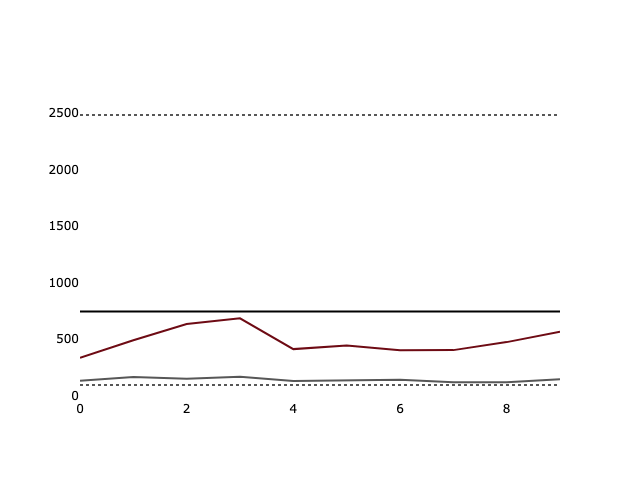
\includegraphics[width=\linewidth]{plots/prompt_1/prompt_1-command_r-cnn_dailymail/prompt_1-command_r-cnn_dailymail_t_word.png}
        \caption{Command-R+\\Total Words}
        \label{fig-command-r-t-word}
    \end{minipage}
    \hfill
    \begin{minipage}{0.32\textwidth}
        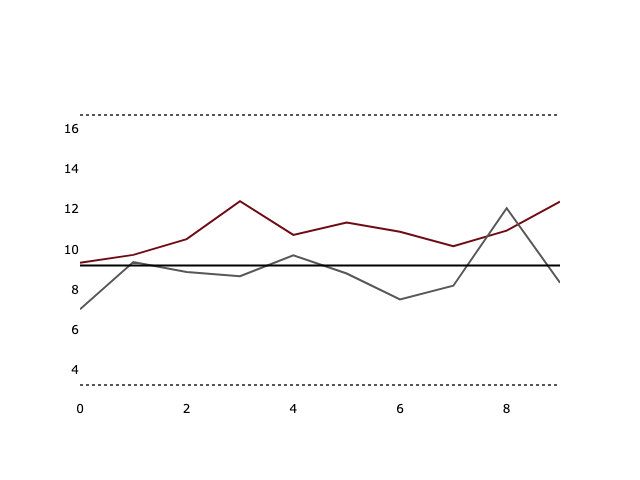
\includegraphics[width=\linewidth]{plots/prompt_1/prompt_1-gpt-cnn_dailymail/prompt_1-gpt-cnn_dailymail_fkgl.png}
        \caption{GPT\\Flesch-Kincaid Grade Level}
        \label{fig-gpt-fkgl}
    \end{minipage}
    \hfill
    \begin{minipage}{0.32\textwidth}
        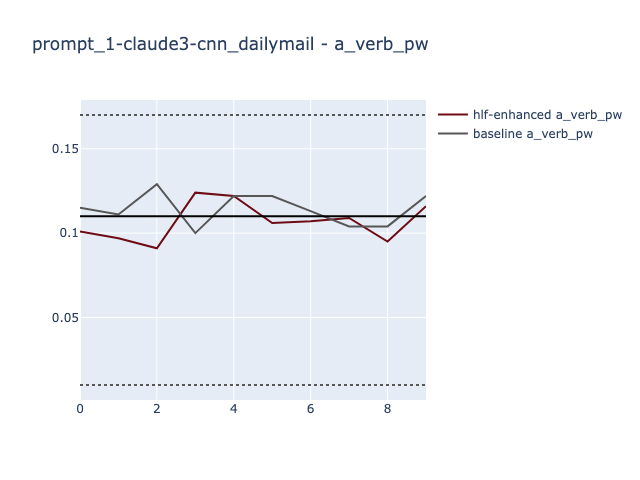
\includegraphics[width=\linewidth]{plots/prompt_1/prompt_1-claude3-cnn_dailymail/prompt_1-claude3-cnn_dailymail_a_verb_pw.png}
        \caption[center]{Claude3\\Average Verbs per Word}
        \label{fig-llama-simp-ttr}
    \end{minipage}
\end{figure*}

\subsection{HLF Instructions and Context Awareness}

The second type of instructional prompt we feed to the LLM contains three
examples from the corpus.
The hypothesis is that this will influence the baseline result to be closer to
the corpus average.

In this case, it is interesting to see how the LLM generates text based on input
text from both within the corpus that contains the example articles and from
outside the corpus.

In Table~\ref{table-prompt-2-cnn-dailymail} we see the results when an input from
outside the corpus is used.
The outlook is similar for what we saw in the first experiment with GPT
being the least responsive to HLF instructions.

\begin{table*}[hpb]
    \centering
    \resizebox{\textwidth}{!}{%
        \begin{tabular}{lllllllllll}
            model                 & t\_word                      & t\_sent                    & n\_uverb                    & n\_uadj                    & simp\_ttr                 & a\_verb\_pw               & corr\_adj\_var            & corr\_verb\_var           & fkgl                       & a\_kup\_pw                \\
            \toprule
            claude3 $Diff\_N$     & \textbf{\underline{718.49}}  & \textbf{\underline{24.13}} & \textbf{\underline{44.43}}  & \textbf{\underline{23.43}} & \textbf{\underline{0.4}}  & 0.03                      & 0.94                      & \textbf{\underline{0.77}} & 1.2                        & 0.07                      \\ \midrule
            claude3 $Diff\_A$     & \textbf{\underline{2345.54}} & \textbf{\underline{90.18}} & \textbf{\underline{148.36}} & \textbf{\underline{63.6}}  & \textbf{\underline{1.18}} & 0.07                      & 1.36                      & \textbf{\underline{2.55}} & 3.33                       & 0.52                      \\ \midrule
            gemini $Diff\_N$      & \textbf{\underline{785.6}}   & \textbf{\underline{25.8}}  & \textbf{\underline{60.5}}   & \textbf{\underline{41.6}}  & \textbf{\underline{0.41}} & \textbf{\underline{0.05}} & \textbf{\underline{1.95}} & \textbf{\underline{2.67}} & -4.62                      & \textbf{\textit{-1.94}}   \\ \midrule
            gemini $Diff\_A$      & \textbf{\underline{2512.0}}  & \textbf{\underline{81.5}}  & \textbf{\underline{210.34}} & \textbf{\underline{125.7}} & \textbf{\underline{1.25}} & \textbf{\underline{0.09}} & \textbf{\underline{5.84}} & \textbf{\underline{8.05}} & -9.46                      & \textbf{\textit{-5.82}}   \\ \midrule
            gpt $Diff\_N$         & 47.8                         & 5.18                       & 6.13                        & -0.13                      & 0.02                      & 0.0                       & 0.05                      & 0.3                       & 3.06                       & -0.27                     \\ \midrule
            gpt $Diff\_A$         & 77.0                         & 12.5                       & 13.0                        & -4.0                       & 0.04                      & 0.0                       & -0.17                     & 0.77                      & 8.45                       & -0.16                     \\ \midrule
            command\_r $Diff\_N$  & \textbf{\underline{263.51}}  & 5.35                       & \textbf{\underline{25.08}}  & \textbf{\underline{17.37}} & \textbf{\textit{-0.09}}   & -0.01                     & \textbf{\underline{1.74}} & \textbf{\underline{1.42}} & \textbf{\underline{10.46}} & \textbf{\underline{1.56}} \\ \midrule
            command\_r $Diff\_A$  & \textbf{\underline{896.0}}   & 20.5                       & \textbf{\underline{86.0}}   & \textbf{\underline{60.6}}  & \textbf{\textit{-0.21}}   & -0.03                     & \textbf{\underline{5.45}} & \textbf{\underline{4.95}} & \textbf{\underline{31.29}} & \textbf{\underline{5.67}} \\ \midrule
            llama3\_70b $Diff\_N$ & \textbf{\underline{376.0}}   & \textbf{\underline{15.63}} & \textbf{\underline{38.63}}  & 15.74                      & \textbf{\underline{0.24}} & \textbf{\underline{0.06}} & 1.69                      & \textbf{\underline{2.91}} & 0.31                       & -0.3                      \\ \midrule
            llama3\_70b $Diff\_A$ & \textbf{\underline{1088.5}}  & \textbf{\underline{45.0}}  & \textbf{\underline{113.0}}  & 41.0                       & \textbf{\underline{0.65}} & \textbf{\underline{0.18}} & 3.53                      & \textbf{\underline{8.56}} & 0.27                       & -0.68                     \\ \bottomrule
        \end{tabular}%
    }
    \caption{prompt 2 - CNN Results\\Input Outside Corpus}
    \label{table-prompt-2-cnn-dailymail}
\end{table*}

GPT's results would be good if the baseline were very close to the target value.
As we can see in Figure~\ref{fig-p2-gpt-twords}, this is not always the case.
We also notice that Command-R+(fig.~\ref{fig-p2-command-r-simpttr}) and Gemini
(fig.~\ref{fig-p2-gemini-a-kup-pw}) both registered significantly negative
results, in contrast to their performance in our first scenario.

\begin{figure*}[hpb]
    \centering
    \begin{minipage}{0.32\textwidth}
        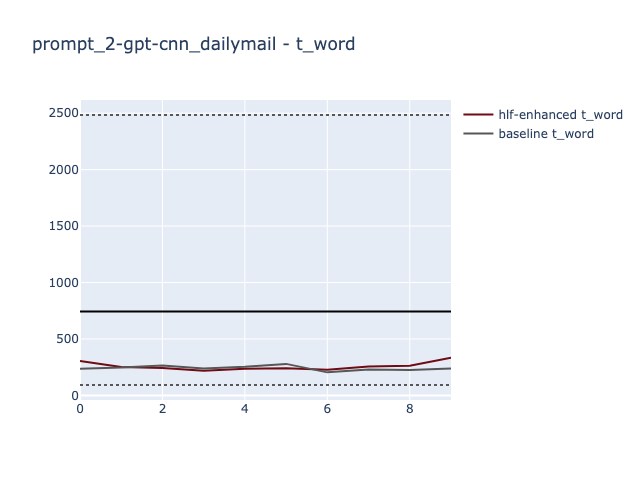
\includegraphics[width=\linewidth]{plots/prompt_2/prompt_2-gpt-cnn_dailymail/prompt_2-gpt-cnn_dailymail_t_word.png}
        \caption{GPT\\Total Words}
        \label{fig-p2-gpt-twords}
    \end{minipage}
    \hfill
    \begin{minipage}{0.32\textwidth}
        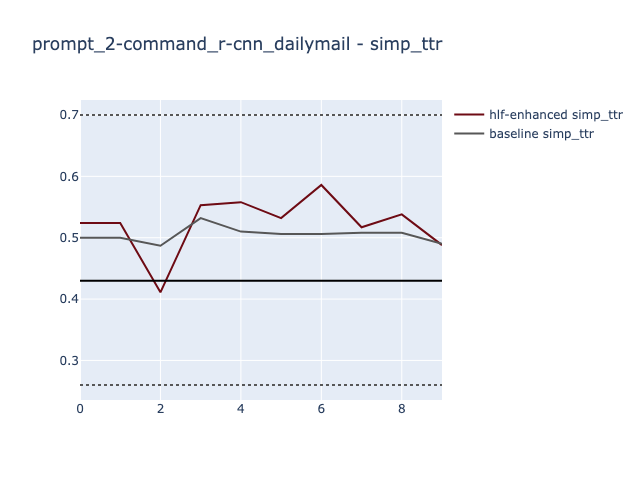
\includegraphics[width=\linewidth]{plots/prompt_2/prompt_2-command_r-cnn_dailymail/prompt_2-command_r-cnn_dailymail_simp_ttr.png}
        \caption{Command-R+\\Simple TTR}
        \label{fig-p2-command-r-simpttr}
    \end{minipage}
    \hfill
    \begin{minipage}{0.32\textwidth}
        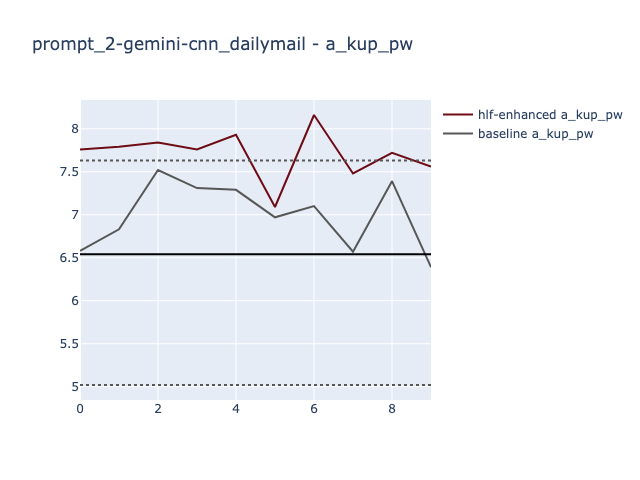
\includegraphics[width=\linewidth]{plots/prompt_2/prompt_2-gemini-cnn_dailymail/prompt_2-gemini-cnn_dailymail_a_kup_pw.png}
        \caption[center]{Gemini\\Kuperman Age of Aquisition}
        \label{fig-p2-gemini-a-kup-pw}
    \end{minipage}
\end{figure*}

The results obtained in our first scenario are largely confirmed by our second
scenario.
So now we turn to see how using a text from within the corpus affects the
performance of the large language models.
The hypothesis is that if the text is `familiar', both the baseline and the HLF
instruction prompt will produce results that are much closer to the target
value.
The expectation is to see less significant results.

\begin{table*}[ht]
    \centering
    \resizebox{\textwidth}{!}{%
        \begin{tabular}{lllllllllll}
            model                 & t\_word                      & t\_sent                     & n\_uverb                    & n\_uadj                    & simp\_ttr                 & a\_verb\_pw               & corr\_adj\_var             & corr\_verb\_var            & fkgl                       & a\_kup\_pw              \\
            \toprule
            claude3 $Diff\_N$     & \textbf{\underline{871.02}}  & \textbf{\underline{34.2}}   & \textbf{\underline{34.48}}  & \textbf{\textit{-7.38}}    & \textbf{\underline{0.27}} & 0.01                      & \textbf{\textit{-0.93}}    & \textbf{\textit{-0.72}}    & 1.16                       & -0.14                   \\ \midrule
            claude3 $Diff\_A$     & \textbf{\underline{2756.12}} & \textbf{\underline{117.18}} & \textbf{\underline{126.36}} & \textbf{\textit{-11.2}}    & \textbf{\underline{0.81}} & -0.01                     & \textbf{\textit{-2.52}}    & \textbf{\textit{-0.74}}    & 3.69                       & -0.4                    \\ \midrule
            gemini $Diff\_N$      & \textbf{\underline{1315.41}} & \textbf{\underline{46.19}}  & \textbf{\underline{114.47}} & \textbf{\underline{72.38}} & \textbf{\underline{1.17}} & 0.03                      & \textbf{\underline{5.25}}  & \textbf{\underline{6.64}}  & -1.6                       & \textbf{\textit{-2.1}}  \\ \midrule
            gemini $Diff\_A$      & \textbf{\underline{3996.0}}  & \textbf{\underline{138.0}}  & \textbf{\underline{357.36}} & \textbf{\underline{212.7}} & \textbf{\underline{3.3}}  & 0.06                      & \textbf{\underline{15.49}} & \textbf{\underline{19.4}}  & -13.22                     & \textbf{\textit{-6.19}} \\ \midrule
            gpt $Diff\_N$         & \textbf{\underline{521.29}}  & \textbf{\underline{23.3}}   & \textbf{\underline{43.13}}  & 19.85                      & \textbf{\underline{0.2}}  & 0.02                      & 1.08                       & \textbf{\underline{1.04}}  & 5.09                       & 0.67                    \\ \midrule
            gpt $Diff\_A$         & \textbf{\underline{1464.0}}  & \textbf{\underline{65.5}}   & \textbf{\underline{121.84}} & 58.1                       & \textbf{\underline{0.58}} & 0.05                      & 2.93                       & \textbf{\underline{2.59}}  & 14.23                      & 1.89                    \\ \midrule
            command\_r $Diff\_N$  & \textbf{\underline{371.08}}  & \textbf{\underline{13.31}}  & 22.06                       & \textbf{\underline{17.19}} & \textbf{\underline{0.17}} & \textbf{\underline{0.02}} & 0.88                       & 1.09                       & \textbf{\underline{4.05}}  & -0.15                   \\ \midrule
            command\_r $Diff\_A$  & \textbf{\underline{1198.0}}  & \textbf{\underline{42.5}}   & 73.0                        & \textbf{\underline{56.5}}  & \textbf{\underline{0.69}} & \textbf{\underline{0.07}} & 2.85                       & 3.99                       & \textbf{\underline{13.89}} & -0.11                   \\ \midrule
            llama3\_70b $Diff\_N$ & \textbf{\underline{1040.85}} & \textbf{\underline{41.99}}  & \textbf{\underline{80.58}}  & \textbf{\underline{49.12}} & \textbf{\underline{0.55}} & \textbf{\underline{0.04}} & \textbf{\underline{3.99}}  & \textbf{\underline{5.05}}  & 7.18                       & \textbf{\textit{-1.94}} \\ \midrule
            llama3\_70b $Diff\_A$ & \textbf{\underline{2928.0}}  & \textbf{\underline{118.5}}  & \textbf{\underline{222.0}}  & \textbf{\underline{133.5}} & \textbf{\underline{1.43}} & \textbf{\underline{0.05}} & \textbf{\underline{10.77}} & \textbf{\underline{13.42}} & 17.21                      & \textbf{\textit{-6.2}}  \\ \bottomrule
        \end{tabular}%
    }
    \caption{CNN Results\\Input Inside Corpus}
    \label{table-prompt-2-ifd-cnn-dailymail}
\end{table*}

The results shown in Table~\ref{table-prompt-2-ifd-cnn-dailymail} contradict our
expectations outright.
The most surprising behaviour is exhibited in the context of more concrete HLFs
such as the total number of words or the number of unique adjectives.
Claude3 shows regressive behaviour for the number of unique adjectives in
Figure~\ref{fig-p2-ifd-claude3-nuadj}, while Gemini constructs texts using a
very different amount of words in Figure~\ref{fig-p2-ifd-gemini-twords}.
Less surprisingly, Llama3 fails to generate text that conforms to the correct
Kuperman age of acquisition per word in Figure~\ref{fig-p2-ifd-llama3-a-kup-pw}.

\begin{figure*}[ht]
    \centering
    \begin{minipage}{0.32\textwidth}
        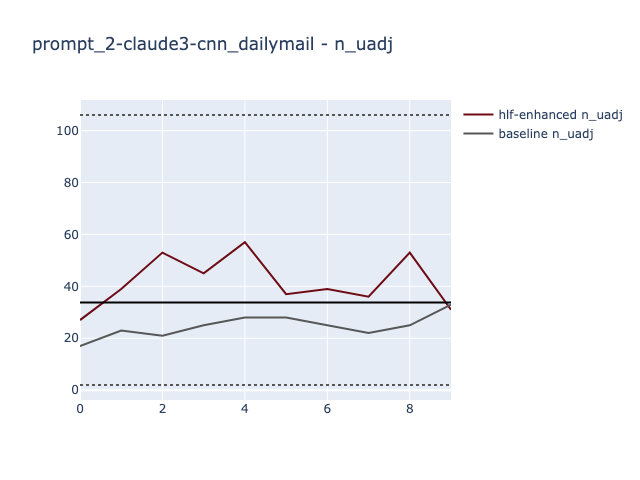
\includegraphics[width=\linewidth]{plots/prompt_2_ifd/prompt_2-claude3-cnn_dailymail/prompt_2-claude3-cnn_dailymail_n_uadj.png}
        \caption{Claude3\\Number of Unique Adjectives}
        \label{fig-p2-ifd-claude3-nuadj}
    \end{minipage}
    \hfill
    \begin{minipage}{0.32\textwidth}
        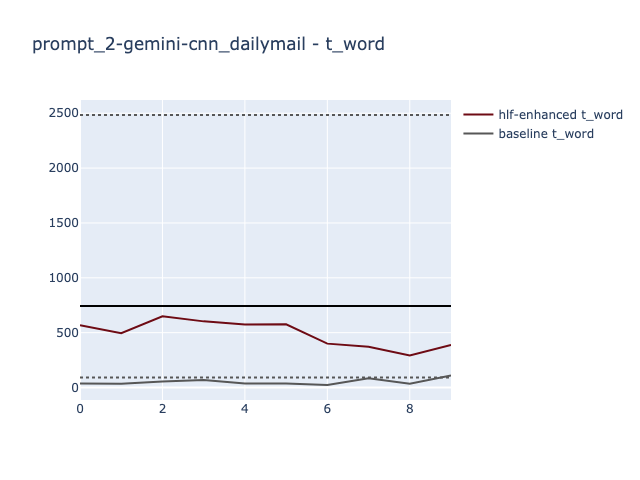
\includegraphics[width=\linewidth]{plots/prompt_2_ifd/prompt_2-gemini-cnn_dailymail/prompt_2-gemini-cnn_dailymail_t_word.png}
        \caption{Gemini\\Total Words}
        \label{fig-p2-ifd-gemini-twords}
    \end{minipage}
    \hfill
    \begin{minipage}{0.32\textwidth}
        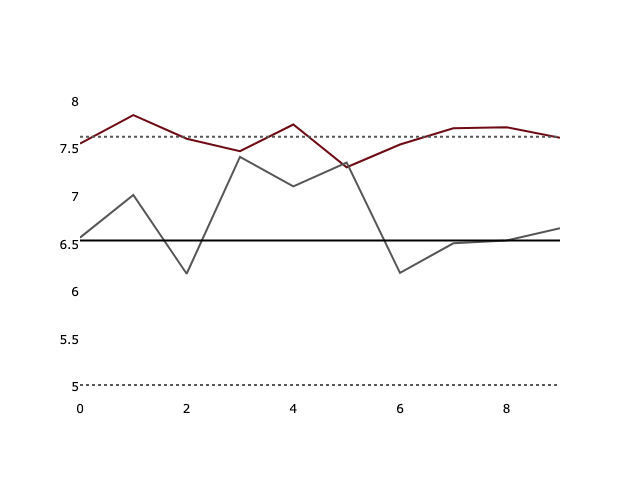
\includegraphics[width=\linewidth]{plots/prompt_2_ifd/prompt_2-llama3_70b-cnn_dailymail/prompt_2-llama3_70b-cnn_dailymail_a_kup_pw.png}
        \caption[center]{Llama3\\Kuperman Age of Aquisition}
        \label{fig-p2-ifd-llama3-a-kup-pw}
    \end{minipage}
\end{figure*}

The results in this last scenario show that whether LLMs take examples listed in
the prompt into account or not with respect to conforming to certain linguistic
features is debatable, providing them with specific instructions derived from
HLFs makes a significant impact.

\section{Discussion}

In terms of our first question --- whether LLMs are able to follow instructions
concerning handcrafted linguistic features --- the response is in our opinion
affirmative.
Certainly, not all LLMs are created equal in this regard.
It is debatable whether this experiment is well designed because of the choice
to derive target HLF values for the LLM from the corpus.
This is evident in the results obtained for the Yelp dataset.
While these results also show a significant influence when using HLFs in the
prompt, the influence is mostly negative.
This can be attributed to the choice of input text in relation to the corpus,
the wording in the instruction prompt or to each model's specific training.

This leads us to our second question: how much do handcrafted linguistic feature
instructions affect the way LLMs write text.
The results in this regards show us a much less conclusive picture.

Firstly, we cannot assume that the LLM will follow HLF instructions the way we
intend.
Whether we obtain the expected outcome or not depends largely on the prompt,
the chosen HLFs, the model, the target values for the HLFs, a.s.o
We do, however, notice a few patterns.
The more abstract the instruction, the less it seems to make a positve impact.
More importantly, by inspecting the result data, a more abstract instruction
seems more likely to produce a negative impact on the desired outcome.

Secondly, the choice of input text in relation to the target HLF values seems
very important.
Choosing to reword a poem so that it has the same reading ease as a user review
seems like a setup for poor results.
This leads us to intuit that LLMs are clearly able to use HLF instructions to
generate text differently, but there is a limit to their `creativity'.

Finally, the choice of HLFs is very important.
The text generated by an LLM is less likely to conform to HLFs that result in
more abstract instructions.
Furthermore, the combination of chosen HLFs is important.
Choosing HLFs that measure the uniqueness of a linguistic element (words,
structures, a.s.o) limits the LLMs ability to conform to other HLFs (for example
total number of sentences or reading ease).
This is highlighted in the experiment specifically in the tension between the
age of acquisition and the adjective or verb variation.
Predictably, the more concrete instructions take precedence over the more
abstract ones.

\section{Conclusions and Future Work}

We started out by trying to understand whether it is possible to conform the
output of a large language model to exhibit specific linguistic features.
To our surprise, it turns out that instructing language models to write text
that conforms to a selected assortment of linguistic features almost always
yields significant changes in how the text is being generated.

This doesn't mean that the results are always satisfying.
What the model writes about and the chosen target values for the linguistic
features are major factors in how successful the overall experience is.
Unfortunately, at this stage, finding out good target values and good writing
instructions is a question of trial and error.

Other experiment designs might have been more opportune in examining the
questions layed out in the introduction.
For example, using set target values for HLFs (without deriving them from a
corpus of text) and choosing input text where the HLFs vary greatly would have
been an alternate design.
Following through on those approaches is one of the possible expansions on the
current work.

Another way of expanding on the current work is finding the settings in which
large language models are most responsive to linguistic features.
The current experiment was inconclusive in this regard and a legitimate further
question is whether settings in which text generated by language models
consistently conforms to certain linguistic features actually exist.

Lastly, a simpler question that is left unanswered relates to the number of
linguistic features that were used.
What if we would have measured models' behaviour for single linguistic features
independently?

\bibliography{references}

\appendix

\section{Additional Result Tables}\label{sec:yelp-tables}
\subsection{Yelp}
\Cref{table-prompt-1-yelp,table-prompt-2-yelp,table-prompt-2-ifd-yelp} show the
experiment results on the corpus of reviews extracted from the Yelp dataset.

\begin{table*}[ht]
    \centering
    \resizebox{\textwidth}{!}{%
        \begin{tabular}{lllllllllll}
            model                 & t\_word                   & t\_sent                    & n\_uverb                 & n\_uadj                  & simp\_ttr & a\_verb\_pw             & corr\_adj\_var          & corr\_verb\_var         & fkgl                       & a\_kup\_pw               \\
            \toprule
            claude3 $Diff\_N$     & \textbf{\textit{-281.9}}  & \textbf{\textit{-13.22}}   & \textbf{\textit{-25.79}} & -14.56                   & -0.06     & 0.0                     & -1.27                   & -1.14                   & \textbf{\underline{6.89}}  & \textbf{\underline{1.0}} \\ \midrule
            claude3 $Diff\_A$     & \textbf{\textit{-774.0}}  & \textbf{\textit{-27.76}}   & \textbf{\textit{-70.0}}  & -38.0                    & -0.19     & 0.02                    & -3.25                   & -3.39                   & \textbf{\underline{21.68}} & \textbf{\underline{2.9}} \\ \midrule
            gemini $Diff\_N$      & -109.27                   & 0.05                       & -7.25                    & -13.18                   & -0.14     & 0.01                    & -1.01                   & -0.4                    & 1.62                       & -0.4                     \\ \midrule
            gemini $Diff\_A$      & -252.82                   & -0.78                      & -17.5                    & -23.14                   & -0.52     & 0.01                    & -1.85                   & -1.07                   & 7.14                       & -0.93                    \\ \midrule
            gpt $Diff\_N$         & -21.62                    & 2.42                       & -3.8                     & -8.84                    & 0.0       & -0.01                   & -0.8                    & -0.53                   & 8.94                       & -0.37                    \\ \midrule
            gpt $Diff\_A$         & -34.72                    & 9.68                       & -10.54                   & -24.57                   & -0.03     & -0.02                   & -2.37                   & -1.58                   & 19.26                      & -1.03                    \\ \midrule
            command\_r $Diff\_N$  & -40.1                     & 1.22                       & 2.43                     & \textbf{\textit{-13.64}} & 0.05      & \textbf{\textit{-0.04}} & \textbf{\textit{-1.17}} & 0.59                    & \textbf{\textit{-7.25}}    & \textbf{\textit{-1.67}}  \\ \midrule
            command\_r $Diff\_A$  & -75.5                     & 1.5                        & 12.94                    & \textbf{\textit{-34.0}}  & 0.19      & \textbf{\textit{-0.12}} & \textbf{\textit{-2.76}} & 2.83                    & \textbf{\textit{-20.49}}   & \textbf{\textit{-4.76}}  \\ \midrule
            llama3\_70b $Diff\_N$ & \textbf{\textit{-210.45}} & \textbf{\underline{6.87}}  & \textbf{\textit{-13.46}} & \textbf{\textit{-15.17}} & -0.16     & \textbf{\textit{-0.02}} & \textbf{\textit{-1.78}} & \textbf{\textit{-1.31}} & 3.7                        & \textbf{\textit{-1.58}}  \\ \midrule
            llama3\_70b $Diff\_A$ & \textbf{\textit{-607.52}} & \textbf{\underline{19.42}} & \textbf{\textit{-41.22}} & \textbf{\textit{-44.77}} & -0.42     & \textbf{\textit{-0.05}} & \textbf{\textit{-5.48}} & \textbf{\textit{-4.34}} & 9.79                       & \textbf{\textit{-4.98}}  \\ \bottomrule
        \end{tabular}%
    }
    \caption{Yelp Results - Prompt Without Examples}
    \label{table-prompt-1-yelp}
\end{table*}

\begin{table*}[!ht]
    \centering
    \resizebox{\textwidth}{!}{%
        \begin{tabular}{lllllllllll}
            model                 & t\_word & t\_sent & n\_uverb & n\_uadj & simp\_ttr & a\_verb\_pw & corr\_adj\_var            & corr\_verb\_var & fkgl                       & a\_kup\_pw \\
            \toprule
            claude3 $Diff\_N$     & -121.77 & -4.61   & -9.9     & 18.41   & -0.11     & 0.03        & \textbf{\underline{1.4}}  & -0.33           & 1.81                       & 0.95       \\ \midrule
            claude3 $Diff\_A$     & -394.5  & -11.5   & -37.5    & 60.0    & -0.37     & 0.09        & \textbf{\underline{4.66}} & -1.49           & 5.38                       & 2.62       \\ \midrule
            gemini $Diff\_N$      & -23.49  & 1.52    & -0.55    & -1.29   & -0.02     & -0.01       & 0.09                      & -0.05           & \textbf{\underline{6.41}}  & 0.2        \\ \midrule
            gemini $Diff\_A$      & -83.0   & 3.0     & -2.5     & -6.36   & -0.0      & -0.03       & 0.26                      & -0.08           & \textbf{\underline{19.63}} & 0.53       \\ \midrule
            gpt $Diff\_N$         & 13.66   & 2.83    & -3.65    & -3.19   & 0.04      & -0.04       & -0.24                     & -0.22           & 7.5                        & 0.0        \\ \midrule
            gpt $Diff\_A$         & 55.5    & 9.5     & -9.86    & -12.86  & 0.14      & -0.11       & -0.84                     & -0.22           & 18.67                      & -0.38      \\ \midrule
            command\_r $Diff\_N$  & -188.71 & 0.69    & -10.73   & 1.17    & -0.23     & -0.01       & \textbf{\underline{0.74}} & -0.83           & \textbf{\textit{-5.02}}    & -0.08      \\ \midrule
            command\_r $Diff\_A$  & -516.82 & 2.02    & -29.22   & 8.28    & -0.66     & -0.0        & \textbf{\underline{2.98}} & -2.48           & \textbf{\textit{-14.52}}   & -0.48      \\ \midrule
            llama3\_70b $Diff\_N$ & -202.95 & -7.84   & -13.73   & 1.43    & -0.15     & -0.04       & 0.38                      & -1.39           & 10.67                      & 1.37       \\ \midrule
            llama3\_70b $Diff\_A$ & -561.24 & -18.78  & -49.94   & 5.07    & -0.38     & -0.14       & 1.62                      & -4.81           & 29.26                      & 3.11       \\ \bottomrule
        \end{tabular}%
    }
    \caption{Yelp Results - Prompt With Examples\\Input External To Corpus}
    \label{table-prompt-2-yelp}
\end{table*}
\begin{table*}[!ht]
    \centering
    \resizebox{\textwidth}{!}{%
        \begin{tabular}{lllllllllll}
            model                 & t\_word                   & t\_sent                 & n\_uverb                  & n\_uadj                  & simp\_ttr               & a\_verb\_pw & corr\_adj\_var          & corr\_verb\_var         & fkgl                    & a\_kup\_pw              \\
            \toprule
            claude3 $Diff\_N$     & -148.13                   & -1.63                   & -3.93                     & \textbf{\textit{-46.03}} & -0.11                   & -0.0        & \textbf{\textit{-3.08}} & -0.31                   & -4.3                    & \textbf{\textit{-1.53}} \\ \midrule
            claude3 $Diff\_A$     & -526.14                   & -7.98                   & -23.86                    & \textbf{\textit{-133.5}} & -0.41                   & -0.0        & \textbf{\textit{-8.98}} & -1.75                   & -21.03                  & \textbf{\textit{-5.34}} \\ \midrule
            gemini $Diff\_N$      & 74.27                     & 0.65                    & 4.67                      & 2.98                     & 0.04                    & -0.0        & -0.22                   & 1.05                    & 1.44                    & -0.65                   \\ \midrule
            gemini $Diff\_A$      & 221.0                     & 2.0                     & 10.5                      & 7.44                     & 0.12                    & -0.03       & -0.85                   & 2.73                    & 3.28                    & -1.79                   \\ \midrule
            gpt $Diff\_N$         & 0.65                      & 4.03                    & -1.19                     & -2.66                    & -0.03                   & -0.01       & -0.17                   & -0.13                   & 1.05                    & -0.67                   \\ \midrule
            gpt $Diff\_A$         & 17.0                      & 11.68                   & -3.68                     & -7.0                     & -0.1                    & -0.04       & -0.43                   & -0.05                   & 0.57                    & -1.75                   \\ \midrule
            command\_r $Diff\_N$  & \textbf{\textit{-236.11}} & \textbf{\textit{-3.6}}  & \textbf{\textit{-0.97}}   & \textbf{\textit{-27.04}} & \textbf{\textit{-0.23}} & 0.0         & -1.24                   & \textbf{\textit{-1.08}} & \textbf{\textit{-2.13}} & \textbf{\textit{-1.09}} \\ \midrule
            command\_r $Diff\_A$  & \textbf{\textit{-727.0}}  & \textbf{\textit{-9.24}} & \textbf{\underline{0.76}} & \textbf{\textit{-68.5}}  & \textbf{\textit{-0.64}} & 0.02        & -2.89                   & \textbf{\textit{-3.08}} & \textbf{\textit{-5.5}}  & \textbf{\textit{-3.0}}  \\ \midrule
            llama3\_70b $Diff\_N$ & \textbf{\textit{-333.03}} & \textbf{\textit{-5.19}} & 4.43                      & \textbf{\textit{-21.38}} & -0.16                   & -0.03       & \textbf{\textit{-1.77}} & -0.03                   & 1.87                    & -0.44                   \\ \midrule
            llama3\_70b $Diff\_A$ & \textbf{\textit{-687.34}} & \textbf{\textit{-3.42}} & 10.7                      & \textbf{\textit{-61.64}} & -0.31                   & -0.04       & \textbf{\textit{-5.6}}  & -0.89                   & 3.0                     & -1.92                   \\ \bottomrule
        \end{tabular}%
    }
    \caption{Yelp Results - Prompt With Examples\\Input From Corpus}
    \label{table-prompt-2-ifd-yelp}
\end{table*}

\section{Additional Plots}

\subsection{GPT}

\Cref{fig:gpt-prompt1-cnn,fig:gpt-prompt1-yelp,fig:gpt-prompt2-cnn,fig:gpt-prompt2-yelp,fig:gpt-prompt2-cnn-ifd,fig:gpt-prompt2-yelp-ifd}
show the experiment results for the Claude 3 Opus large language model.

\begin{figure*}[ht]
    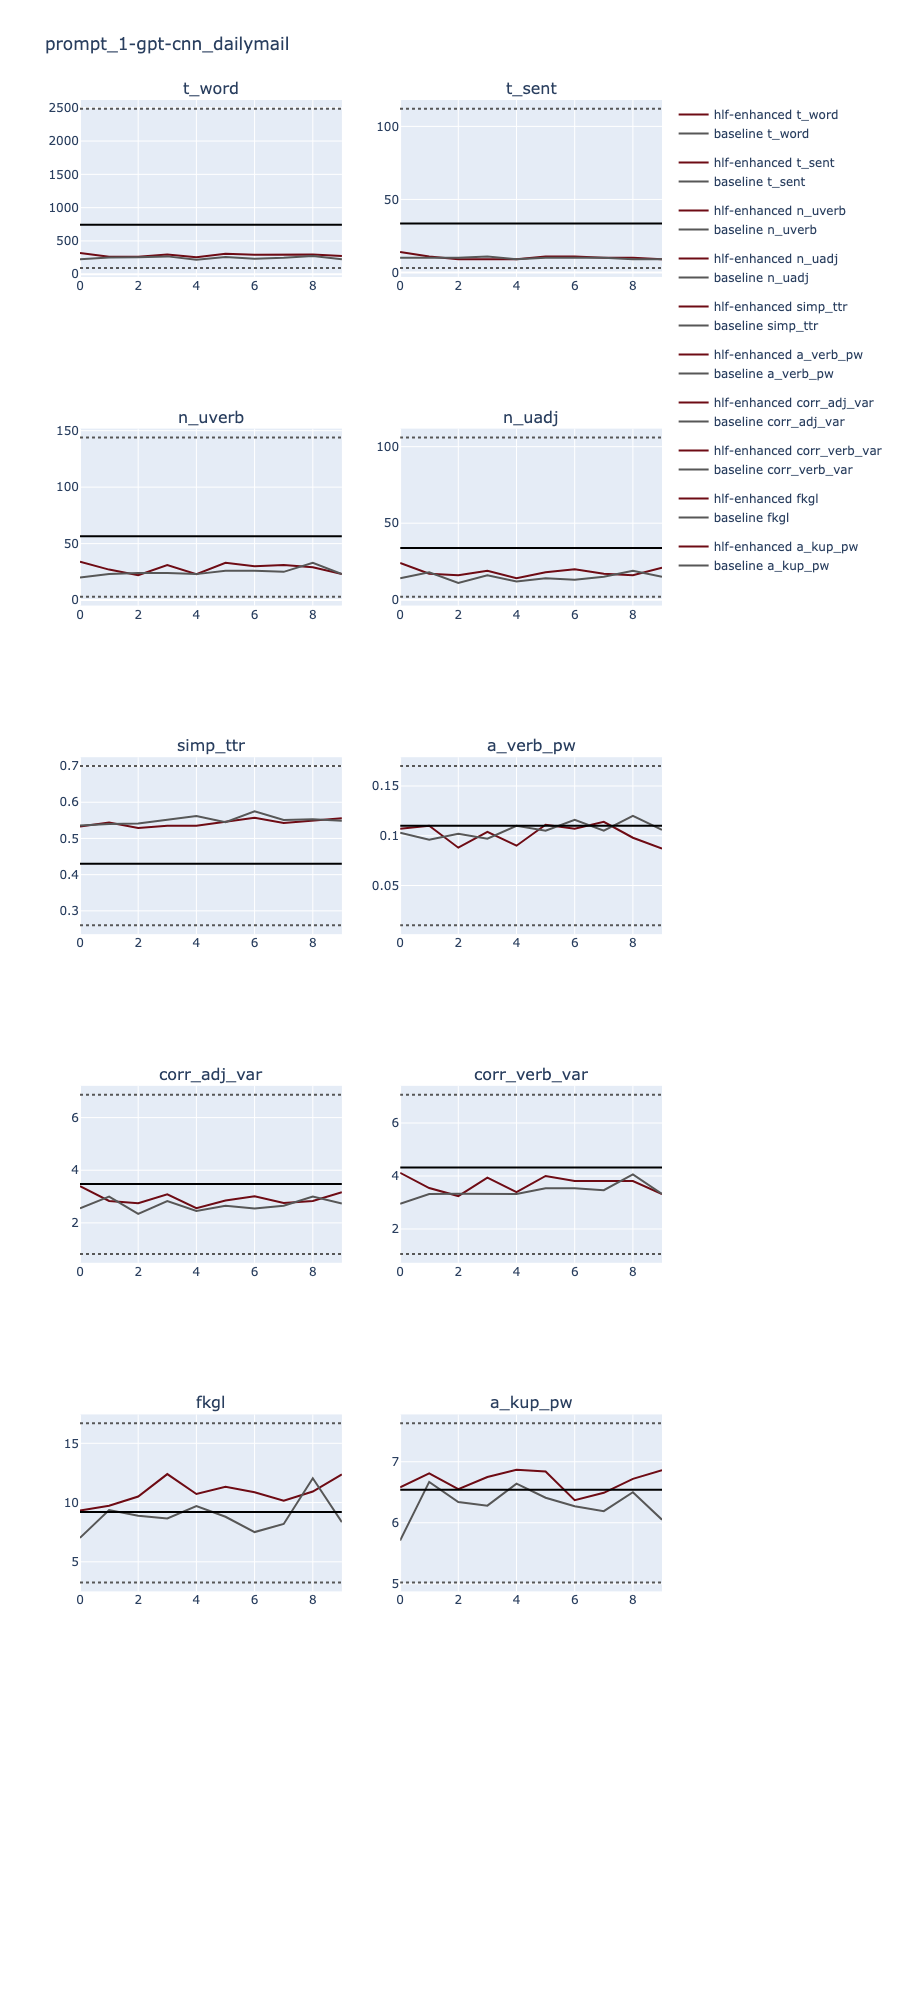
\includegraphics[width=\textwidth,height=0.9\textheight,scale=1]{plots/prompt_1/prompt_1-gpt-cnn_dailymail/prompt_1-gpt-cnn_dailymail.png}
    \caption{GPT on CNN Corpus\\Prompt Without Examples}
    \label{fig:gpt-prompt1-cnn}
\end{figure*}
\begin{figure*}[ht]
    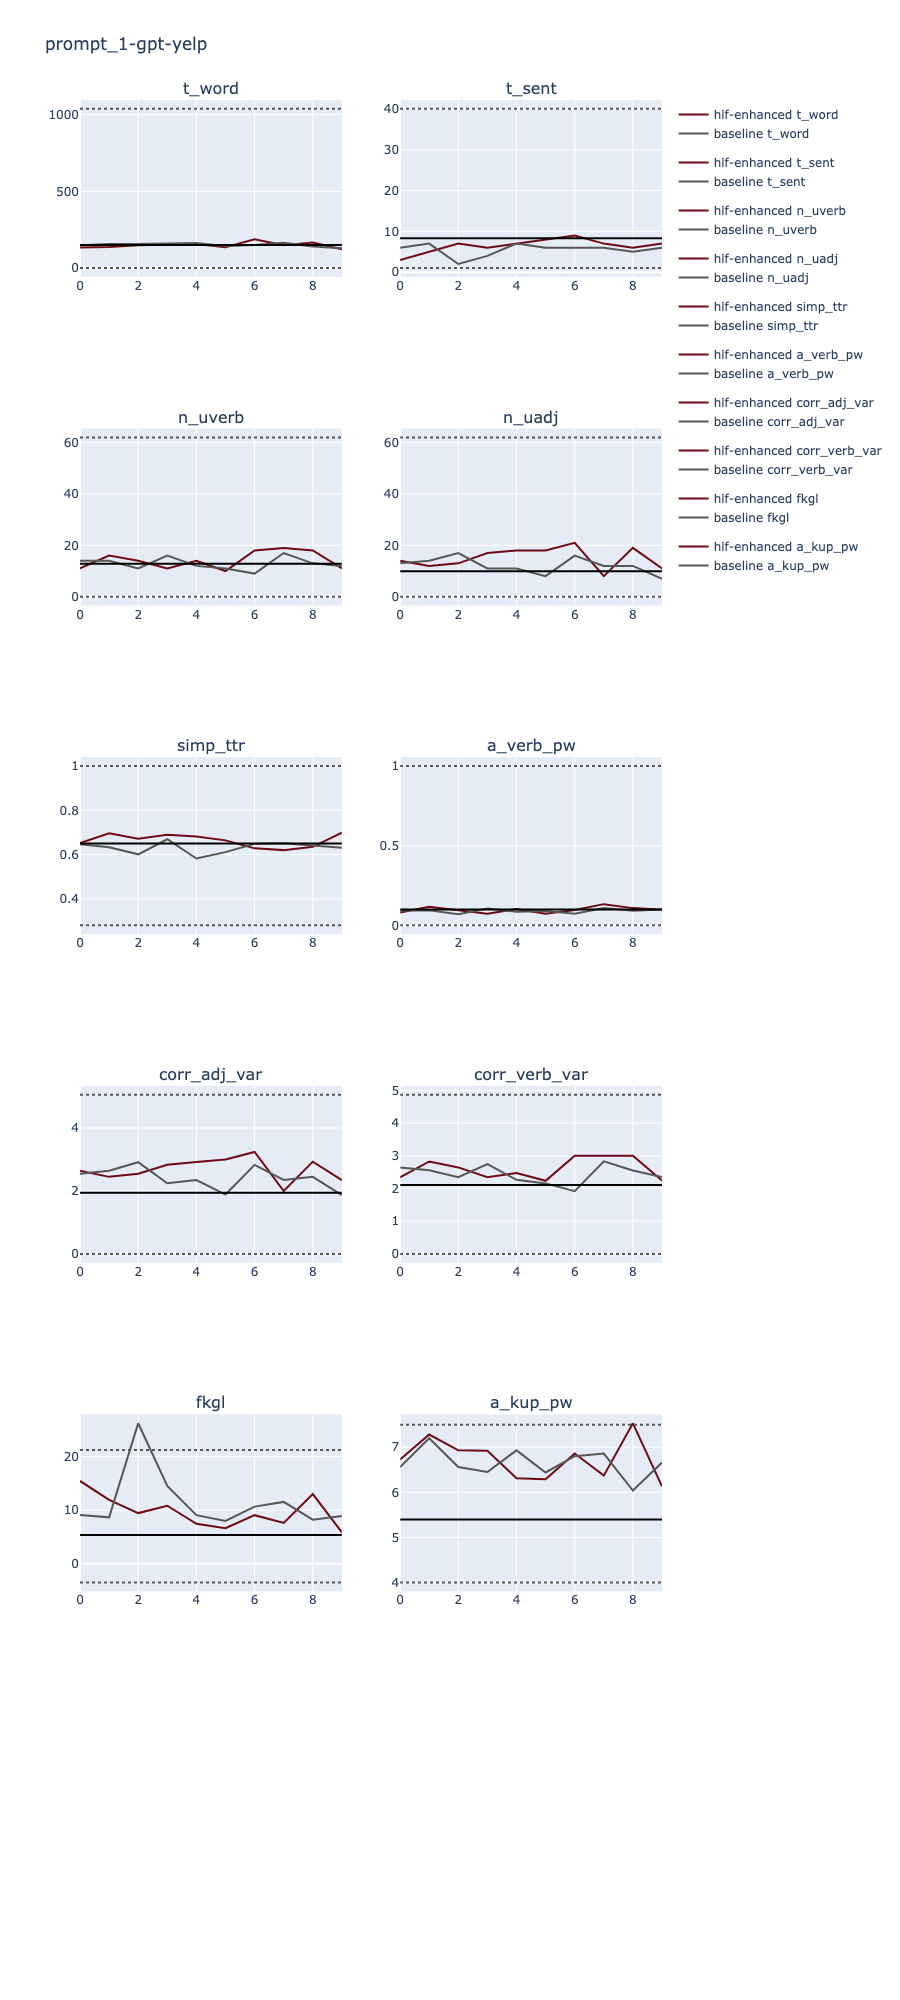
\includegraphics[width=\textwidth,height=0.9\textheight,scale=1]{plots/prompt_1/prompt_1-gpt-yelp/prompt_1-gpt-yelp.png}
    \caption{GPT on Yelp Corpus\\Prompt Without Examples}
    \label{fig:gpt-prompt1-yelp}
\end{figure*}
\begin{figure*}[ht]
    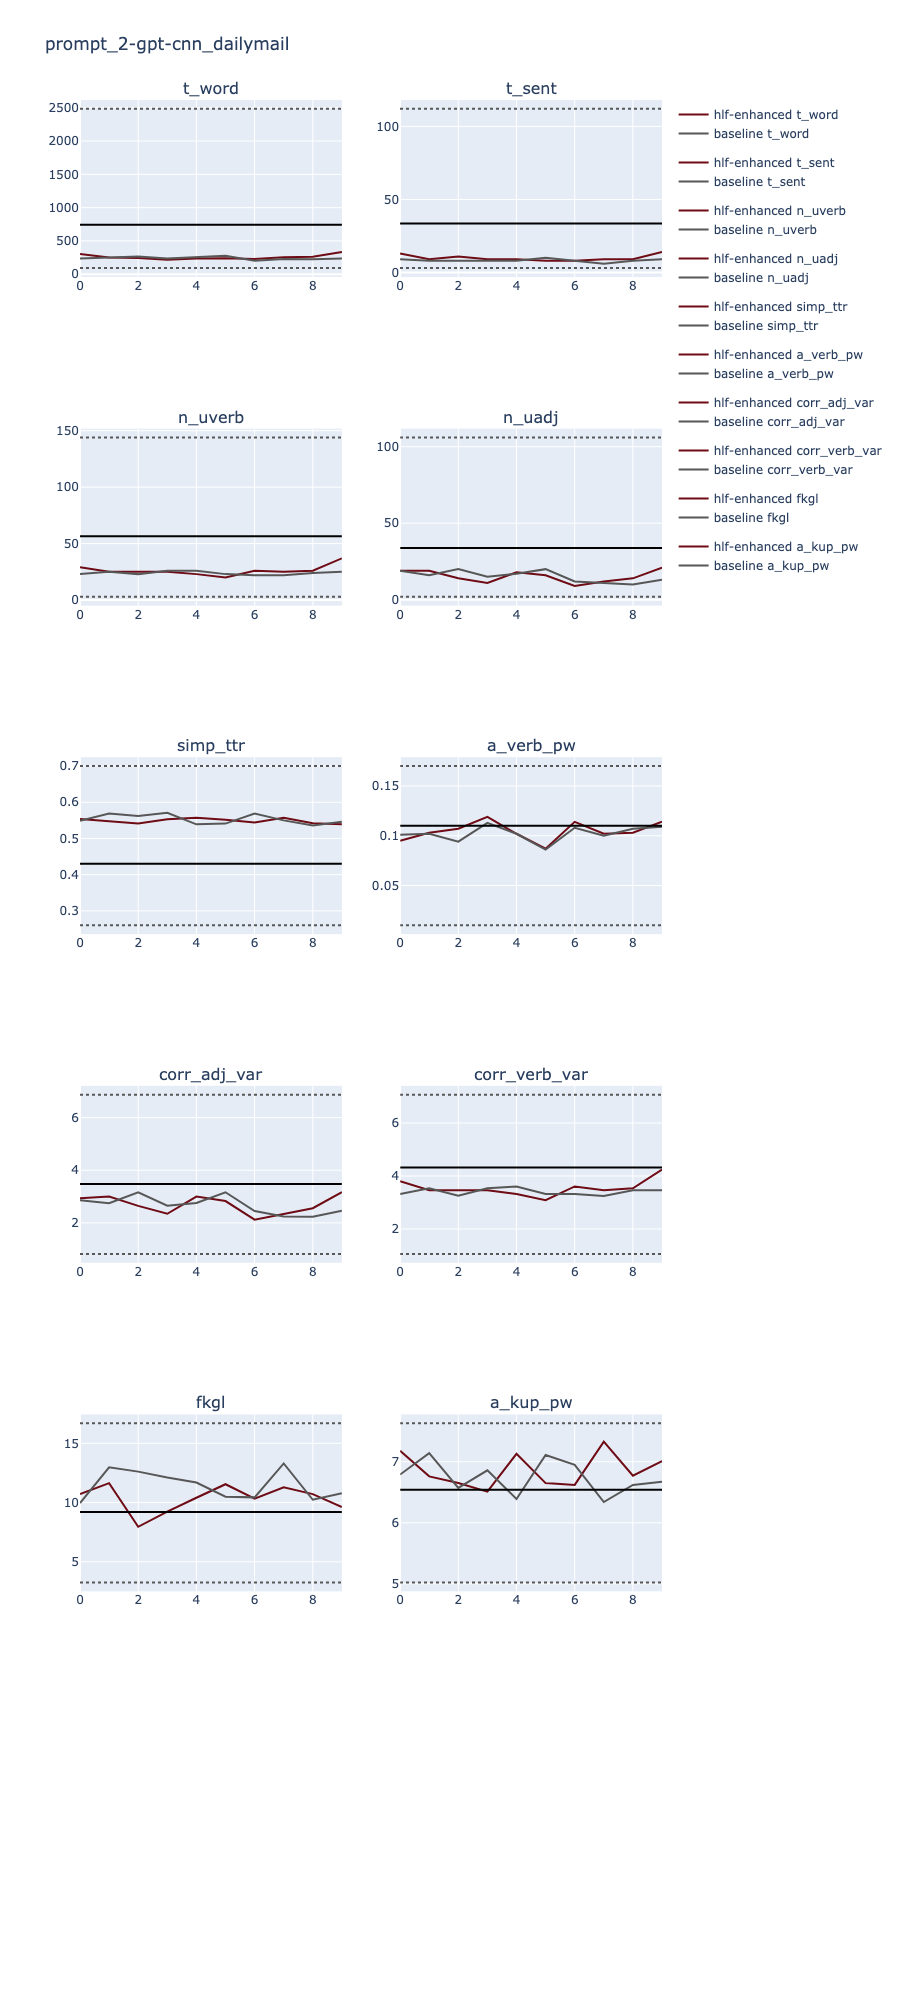
\includegraphics[width=\textwidth,height=0.9\textheight,scale=1]{plots/prompt_2/prompt_2-gpt-cnn_dailymail/prompt_2-gpt-cnn_dailymail.png}
    \caption{GPT on CNN Corpus\\Prompt With Examples\\Extraneous Input}
    \label{fig:gpt-prompt2-cnn}
\end{figure*}
\begin{figure*}[ht]
    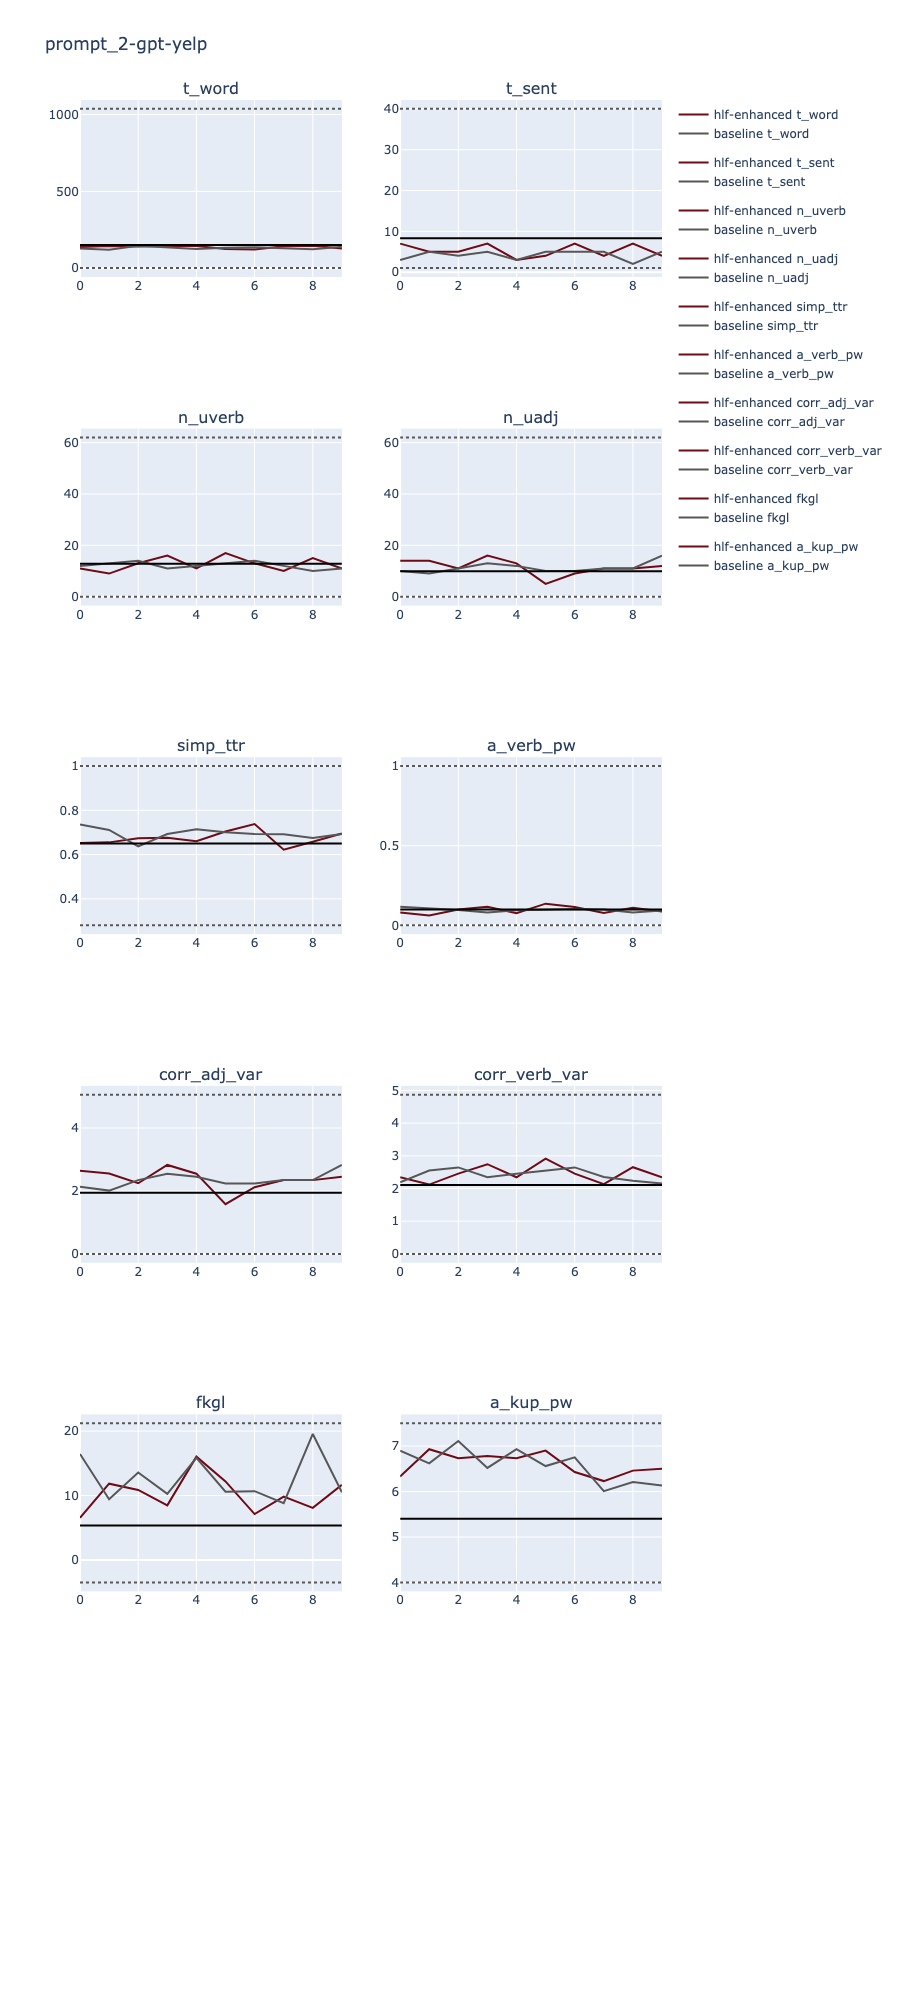
\includegraphics[width=\textwidth,height=0.9\textheight,scale=1]{plots/prompt_2/prompt_2-gpt-yelp/prompt_2-gpt-yelp.png}
    \caption{GPT on Yelp Corpus\\Prompt With Examples\\Extraneous Input}
    \label{fig:gpt-prompt2-yelp}
\end{figure*}
\begin{figure*}[ht]
    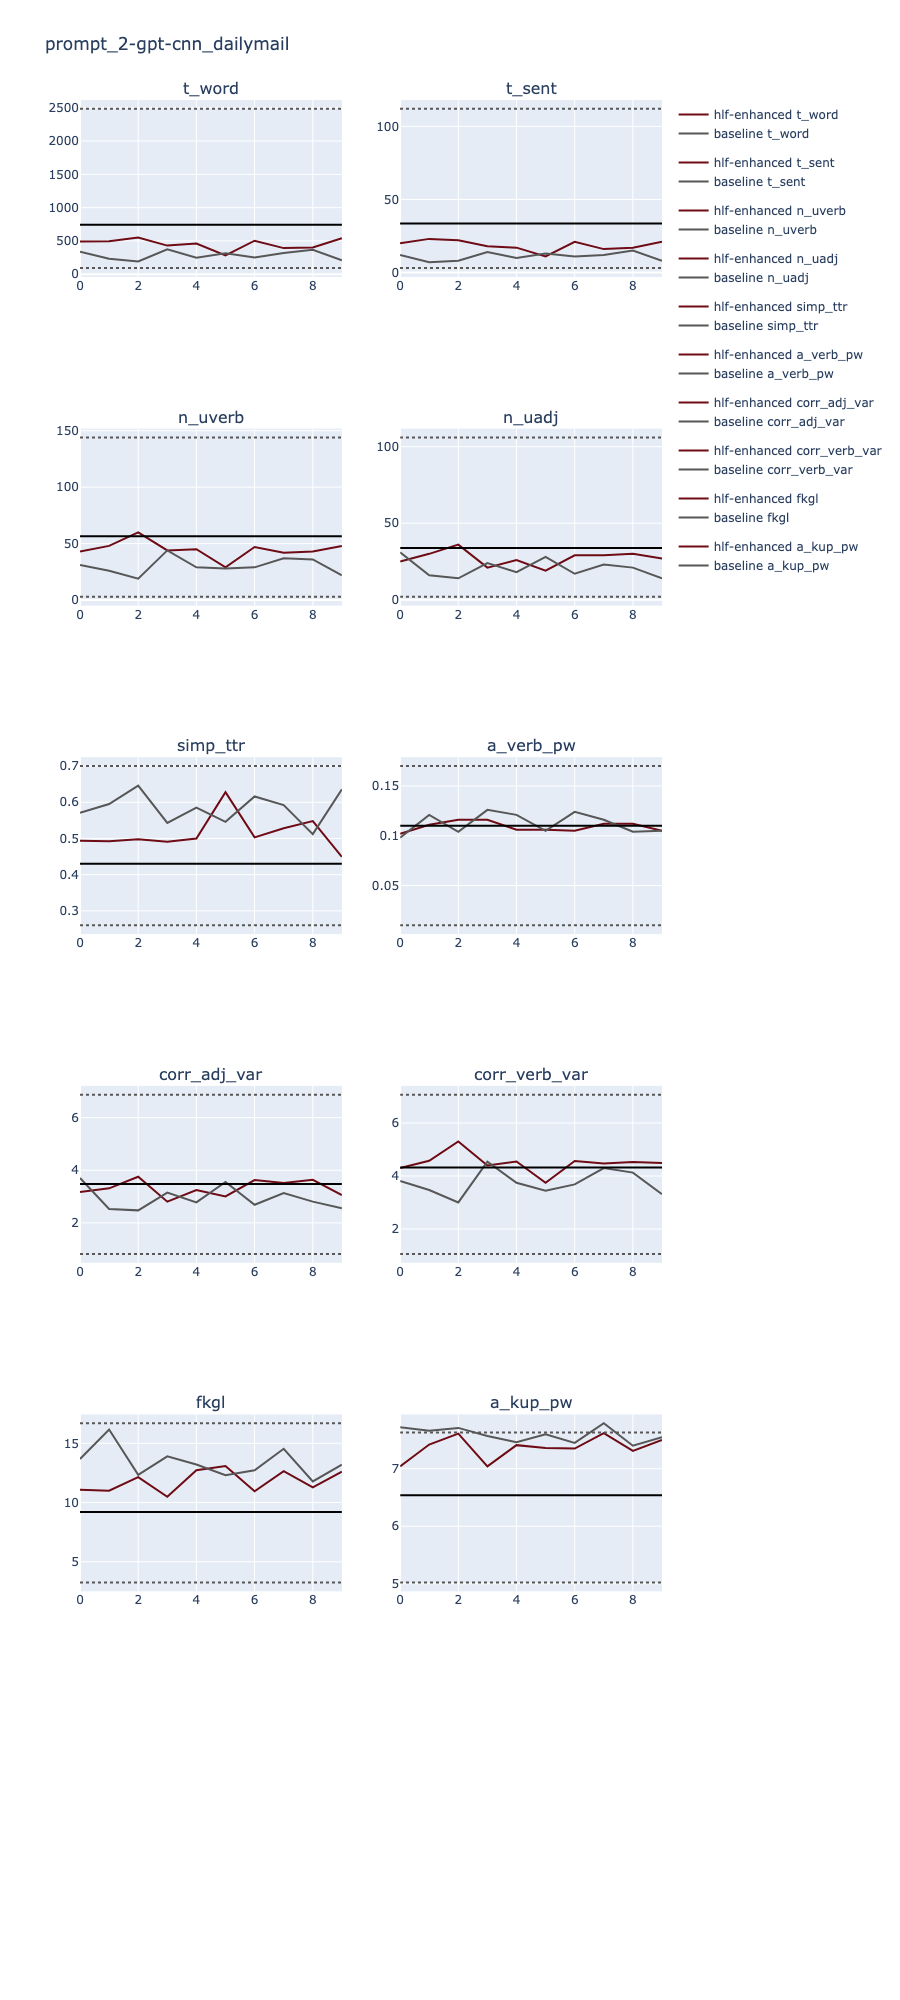
\includegraphics[width=\textwidth,height=0.9\textheight,scale=1]{plots/prompt_2_ifd/prompt_2-gpt-cnn_dailymail/prompt_2-gpt-cnn_dailymail.png}
    \caption{GPT on CNN Corpus\\Prompt With Examples\\Input from Corpus}
    \label{fig:gpt-prompt2-cnn-ifd}
\end{figure*}
\begin{figure*}[ht]
    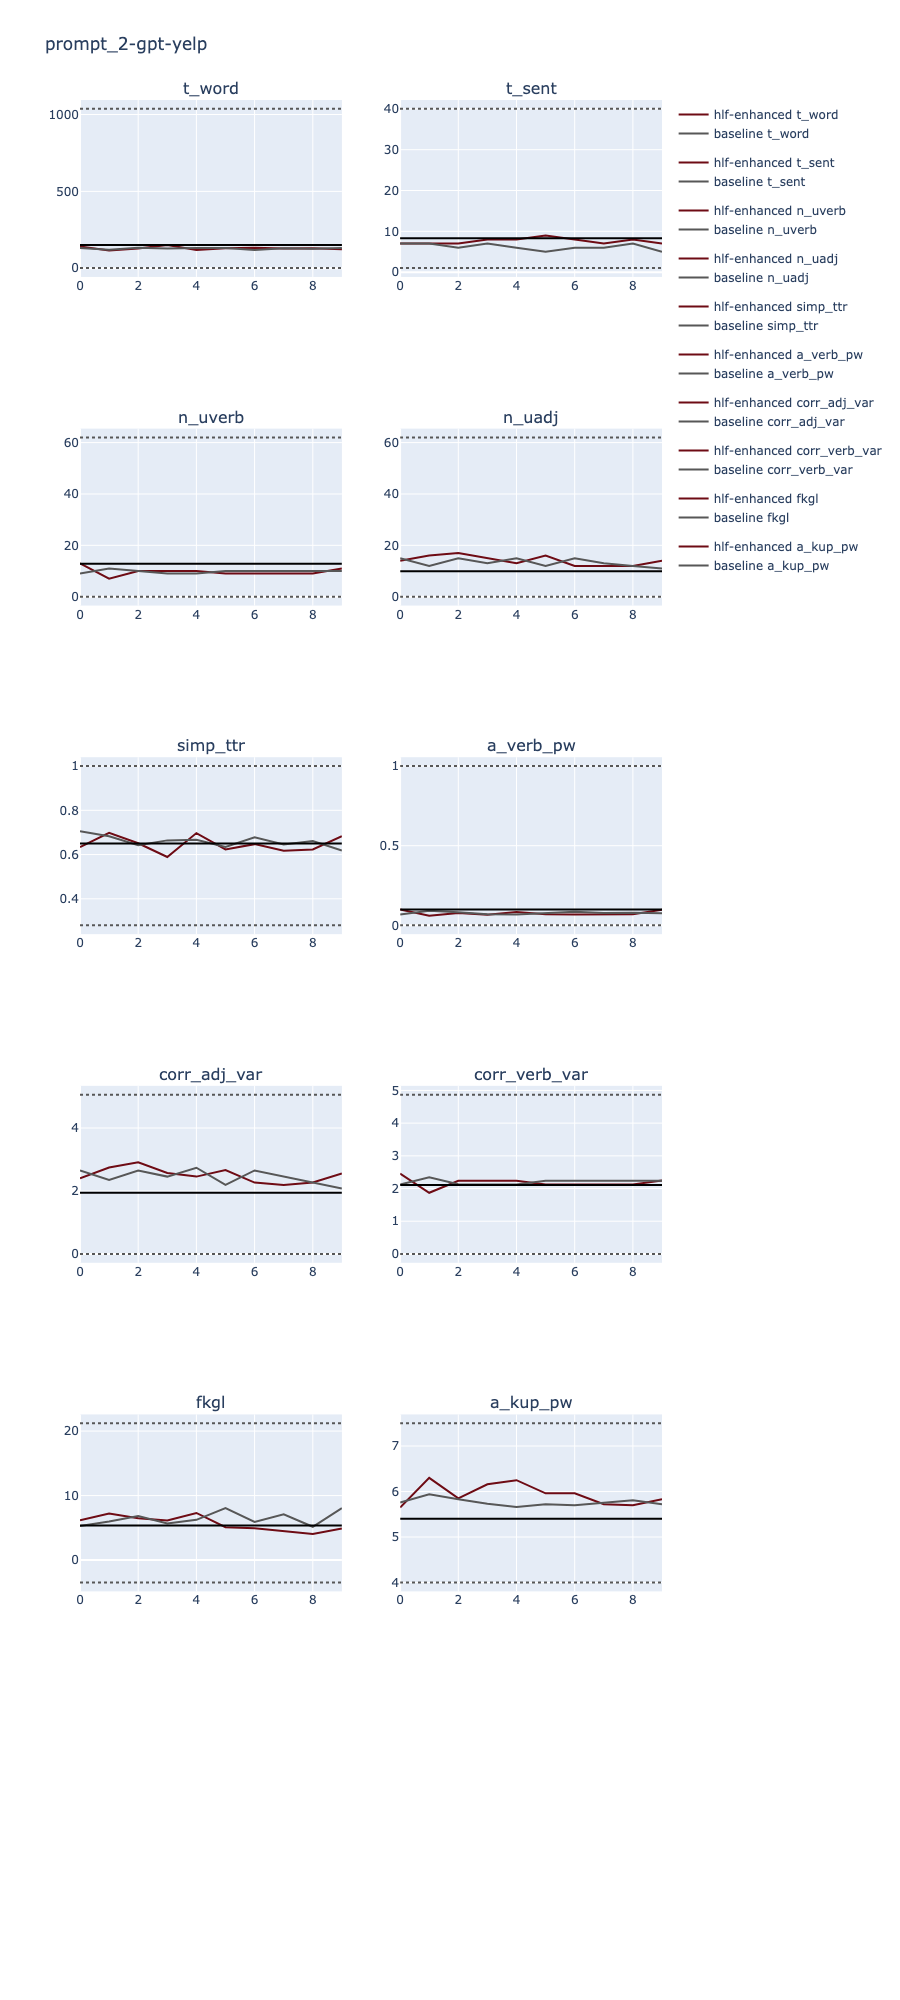
\includegraphics[width=\textwidth,height=0.9\textheight,scale=1]{plots/prompt_2_ifd/prompt_2-gpt-yelp/prompt_2-gpt-yelp.png}
    \caption{GPT on Yelp Corpus\\Prompt With Examples\\Input from Corpus}
    \label{fig:gpt-prompt2-yelp-ifd}
\end{figure*}

\subsection{Gemini}

\Cref{fig:gemini-prompt1-cnn,fig:gemini-prompt1-yelp,fig:gemini-prompt2-cnn,fig:gemini-prompt2-yelp,fig:gemini-prompt2-cnn-ifd,fig:gemini-prompt2-yelp-ifd}
show the experiment results for the Claude 3 Opus large language model.

\begin{figure*}[ht]
    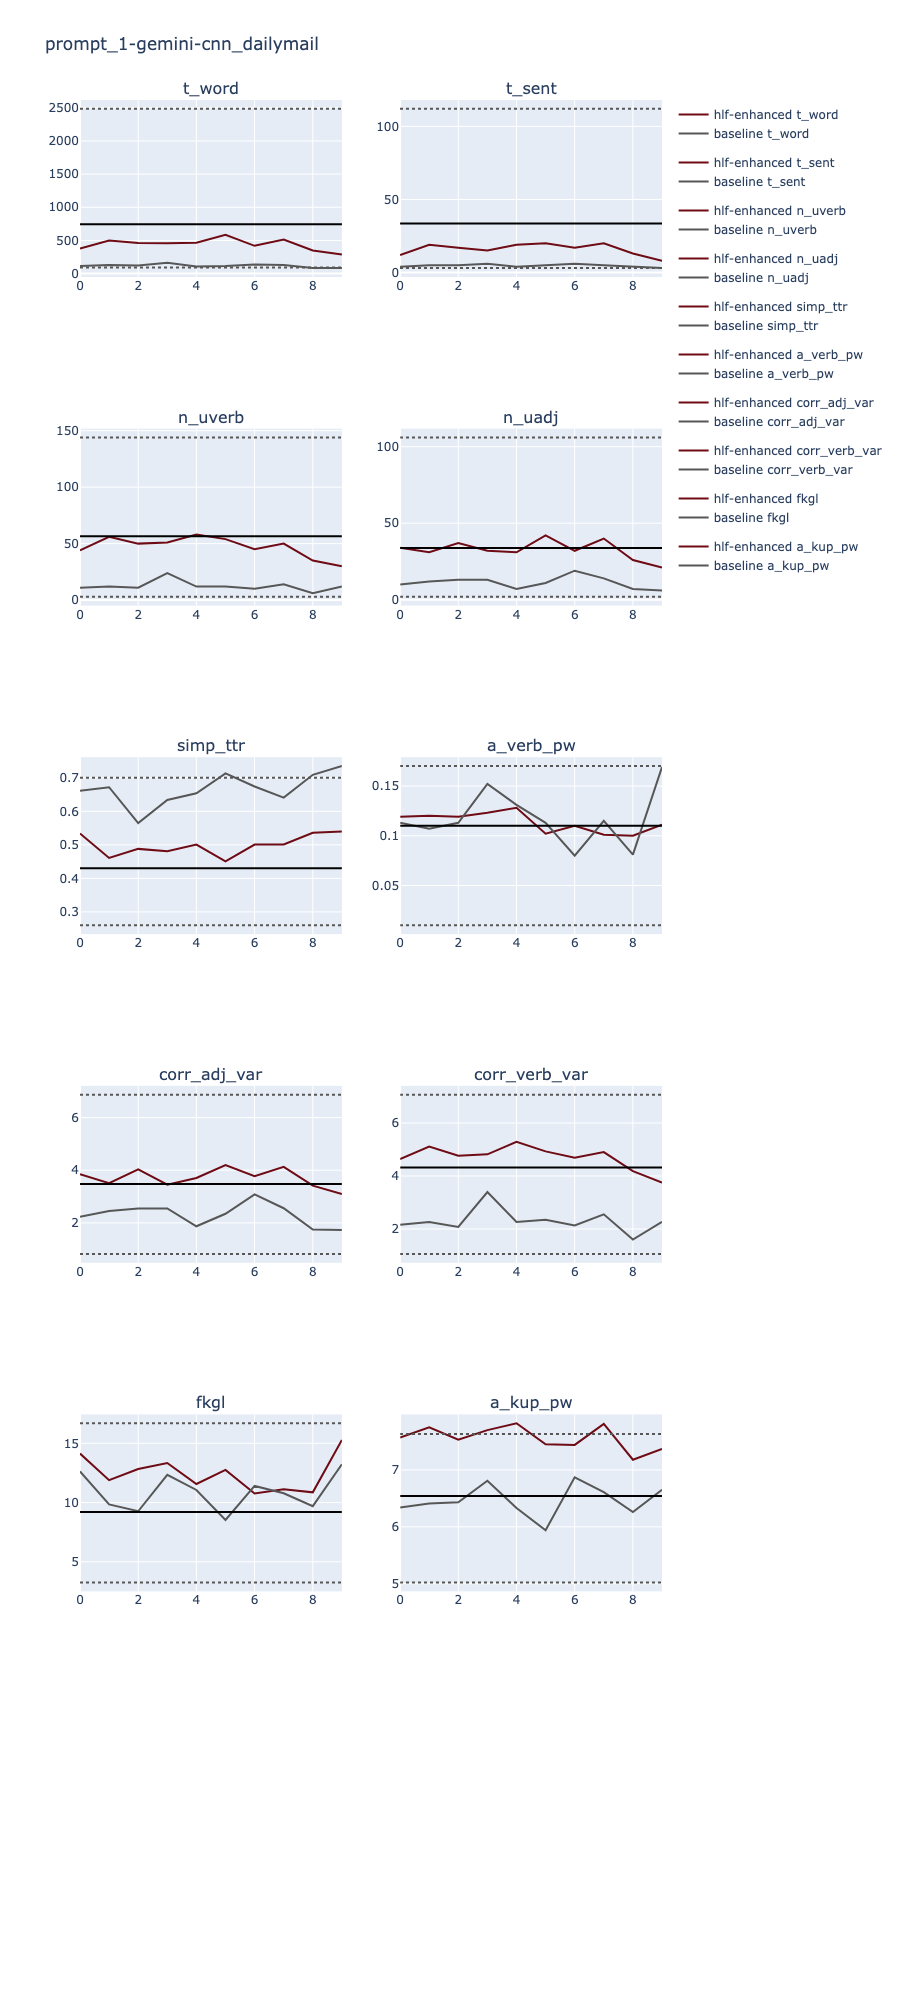
\includegraphics[width=\textwidth,height=0.9\textheight,scale=1]{plots/prompt_1/prompt_1-gemini-cnn_dailymail/prompt_1-gemini-cnn_dailymail.png}
    \caption{Gemini on CNN Corpus\\Prompt Without Examples}
    \label{fig:gemini-prompt1-cnn}
\end{figure*}
\begin{figure*}[ht]
    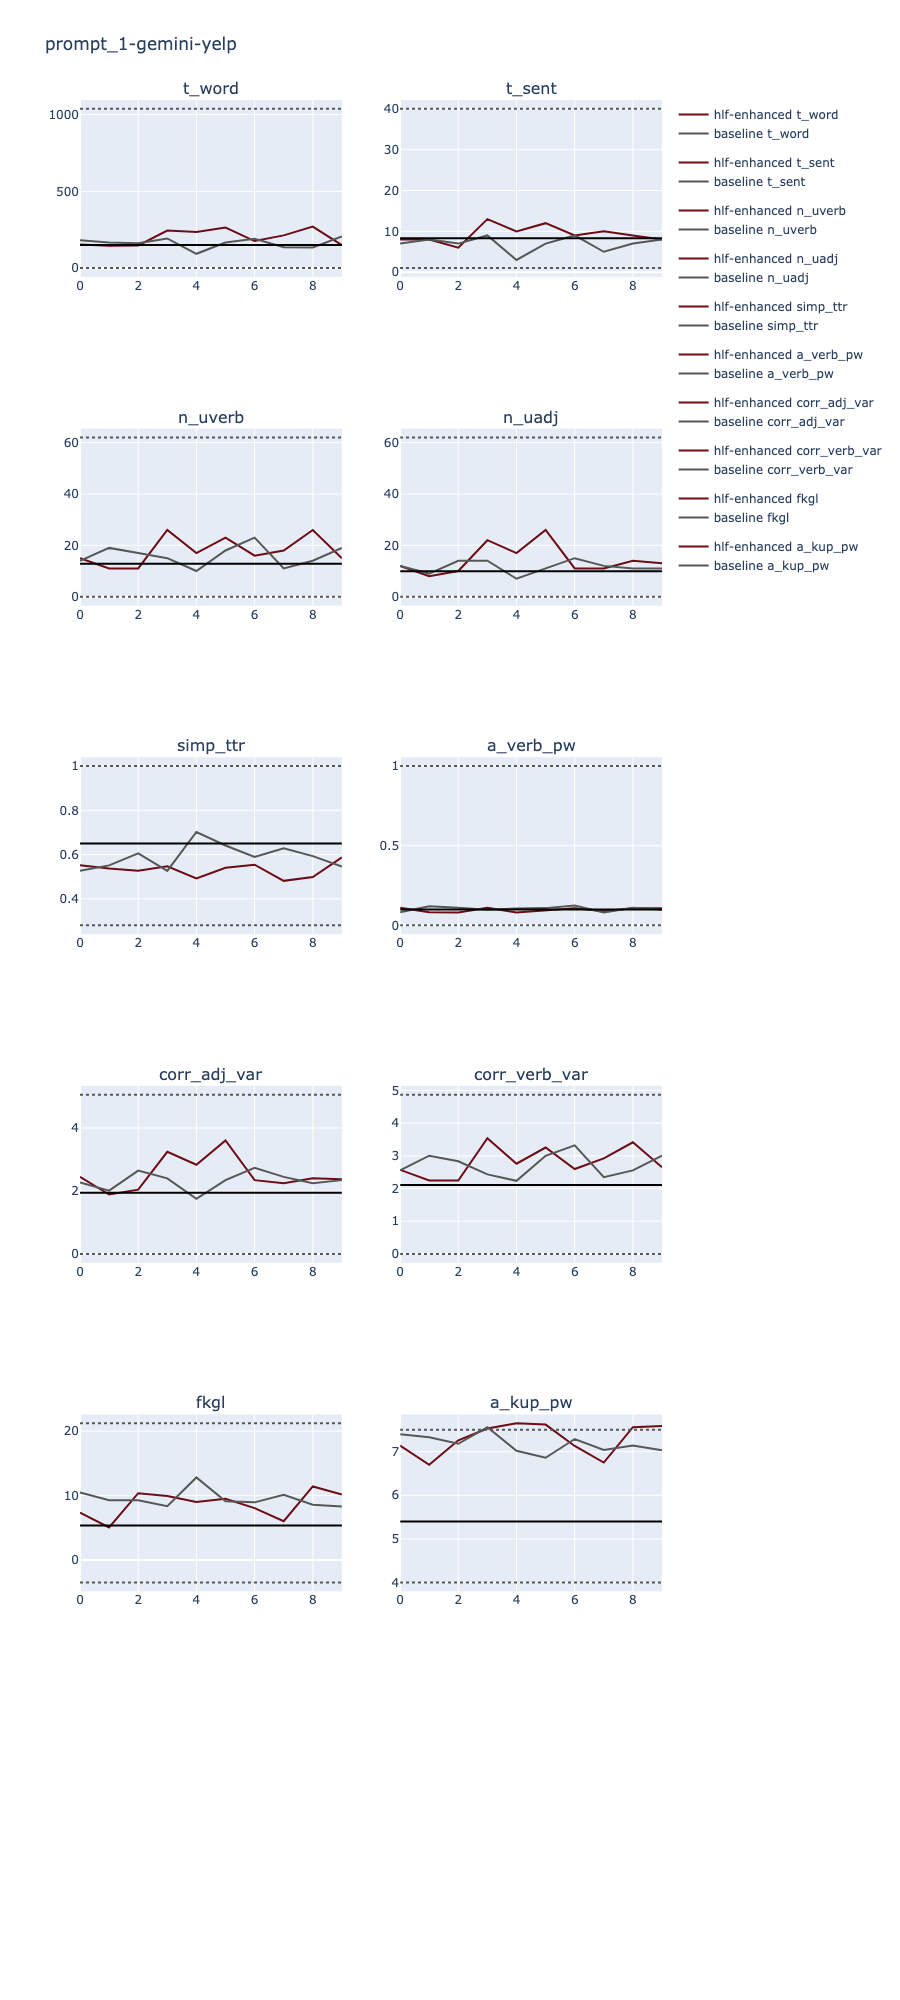
\includegraphics[width=\textwidth,height=0.9\textheight,scale=1]{plots/prompt_1/prompt_1-gemini-yelp/prompt_1-gemini-yelp.png}
    \caption{Gemini on Yelp Corpus\\Prompt Without Examples}
    \label{fig:gemini-prompt1-yelp}
\end{figure*}
\begin{figure*}[ht]
    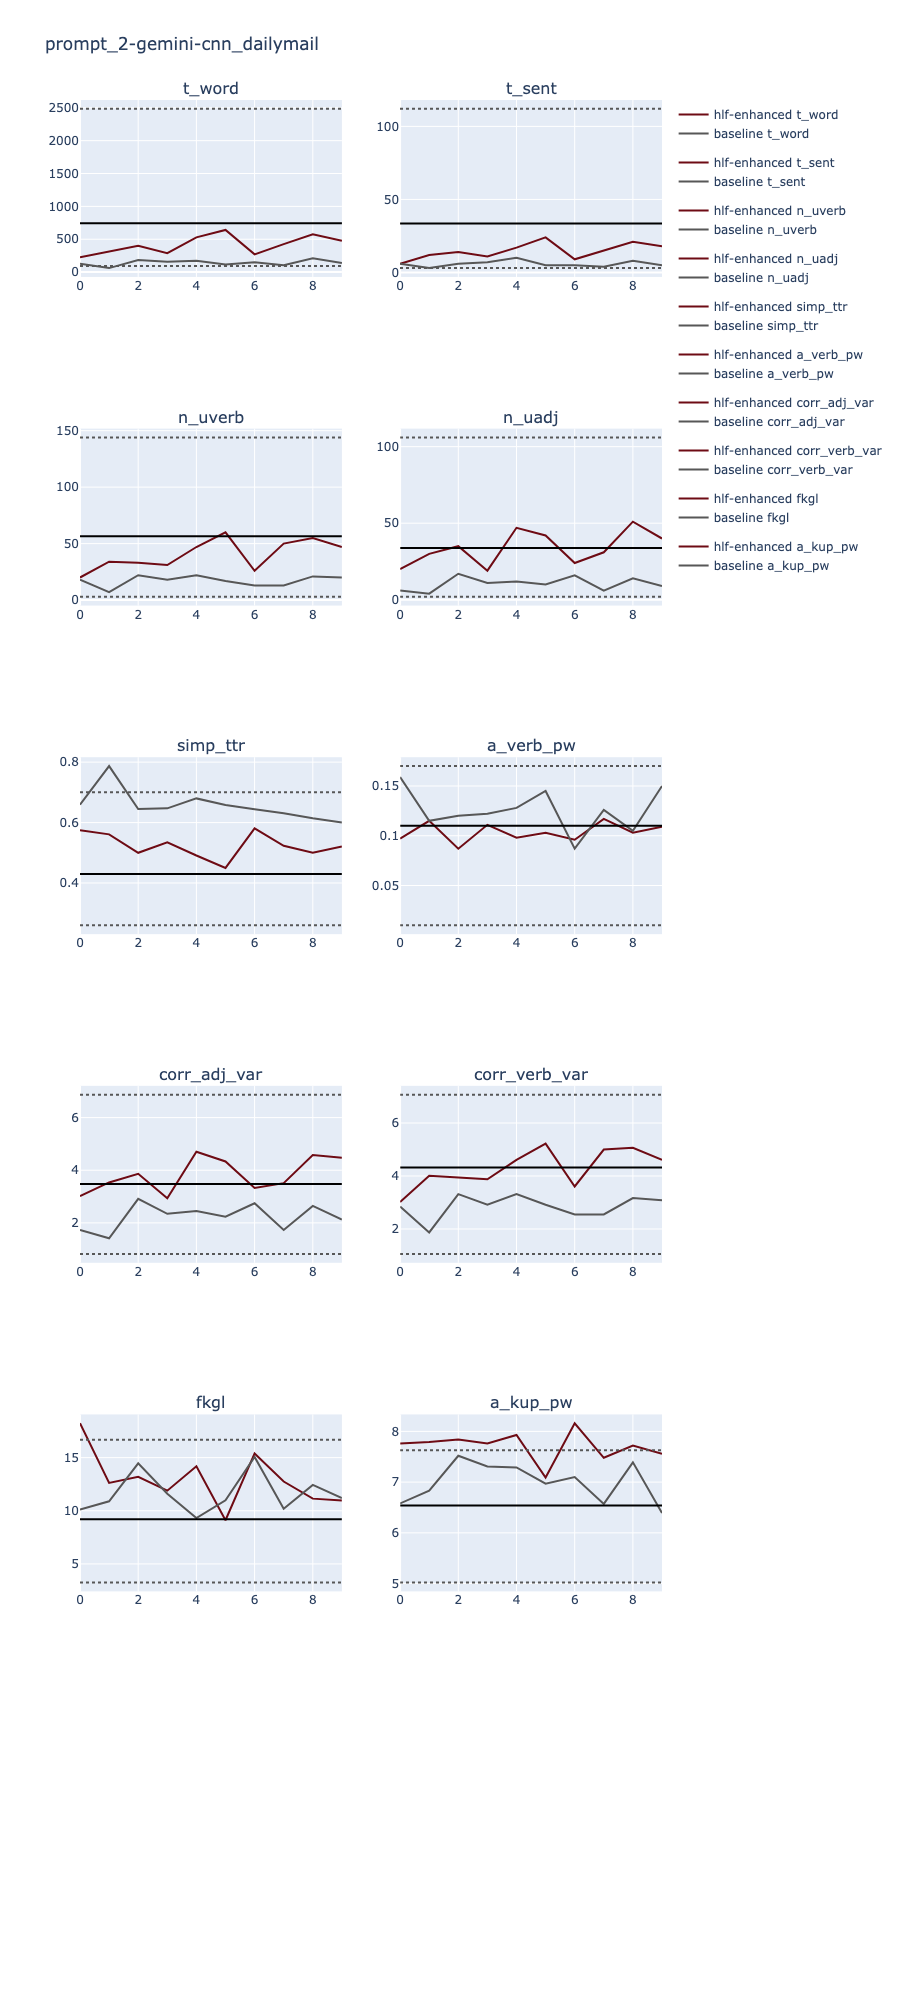
\includegraphics[width=\textwidth,height=0.9\textheight,scale=1]{plots/prompt_2/prompt_2-gemini-cnn_dailymail/prompt_2-gemini-cnn_dailymail.png}
    \caption{Gemini on CNN Corpus\\Prompt With Examples\\Extraneous Input}
    \label{fig:gemini-prompt2-cnn}
\end{figure*}
\begin{figure*}[ht]
    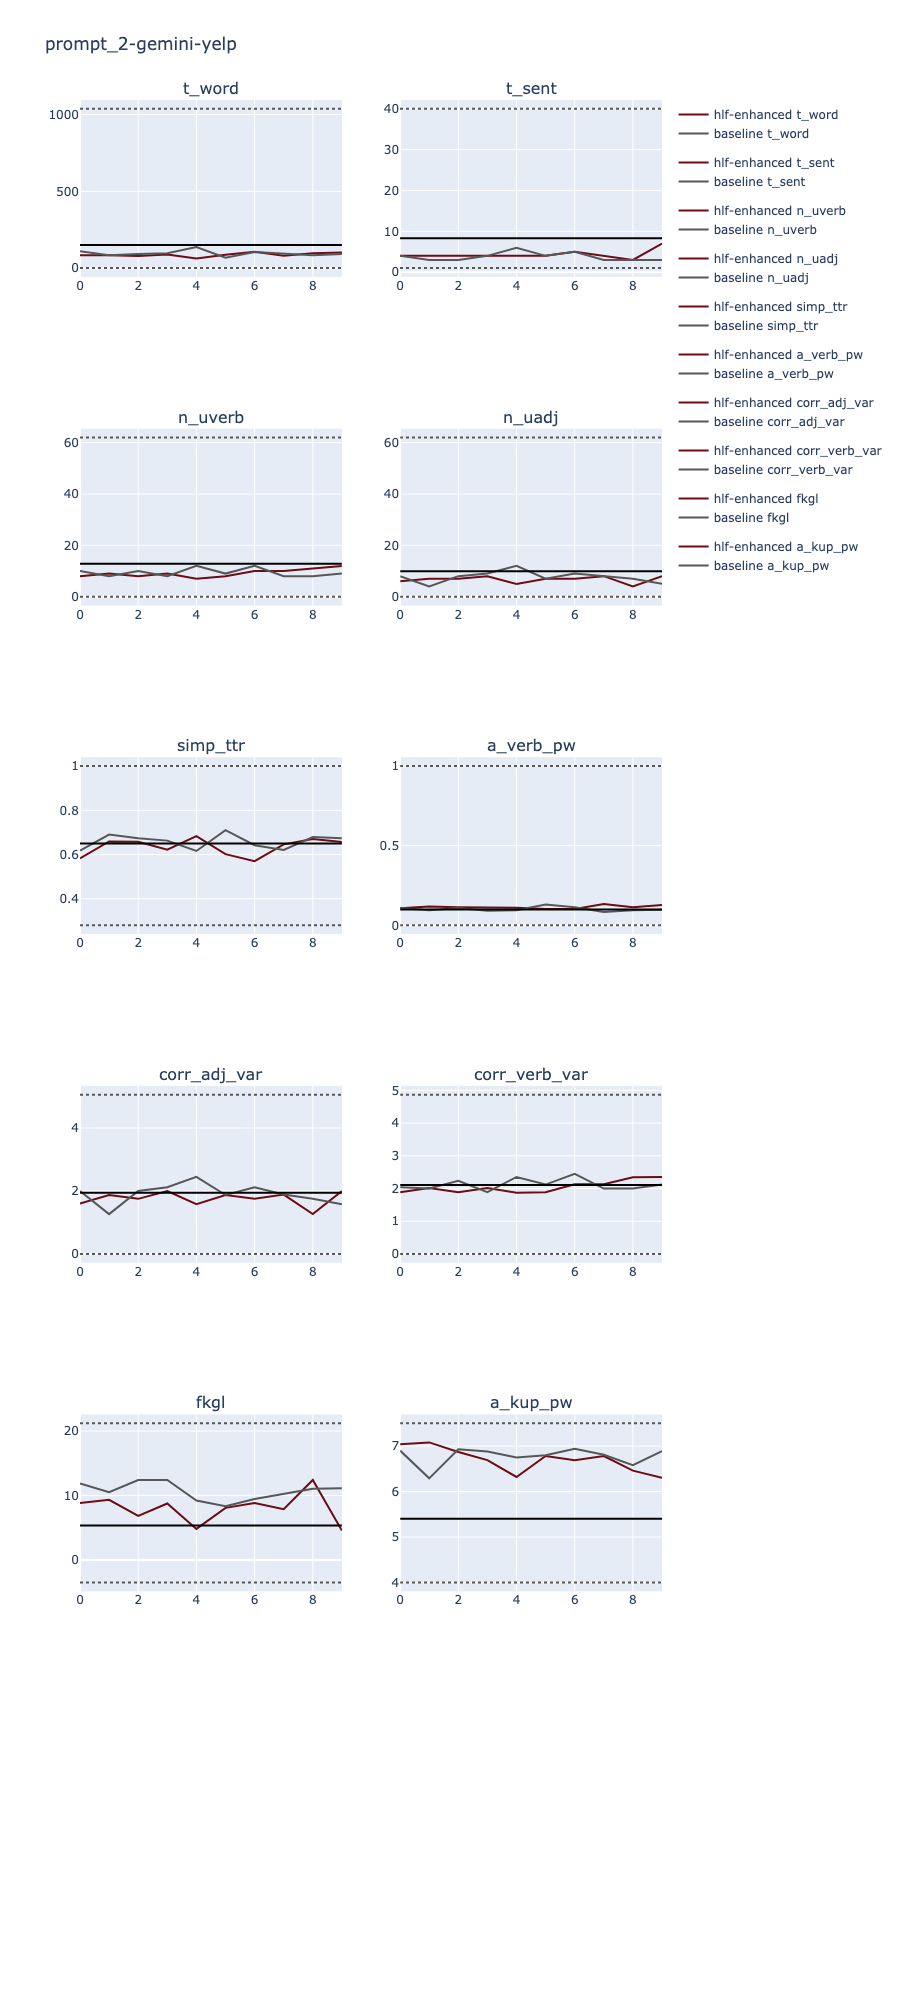
\includegraphics[width=\textwidth,height=0.9\textheight,scale=1]{plots/prompt_2/prompt_2-gemini-yelp/prompt_2-gemini-yelp.png}
    \caption{Gemini on Yelp Corpus\\Prompt With Examples\\Extraneous Input}
    \label{fig:gemini-prompt2-yelp}
\end{figure*}
\begin{figure*}[ht]
    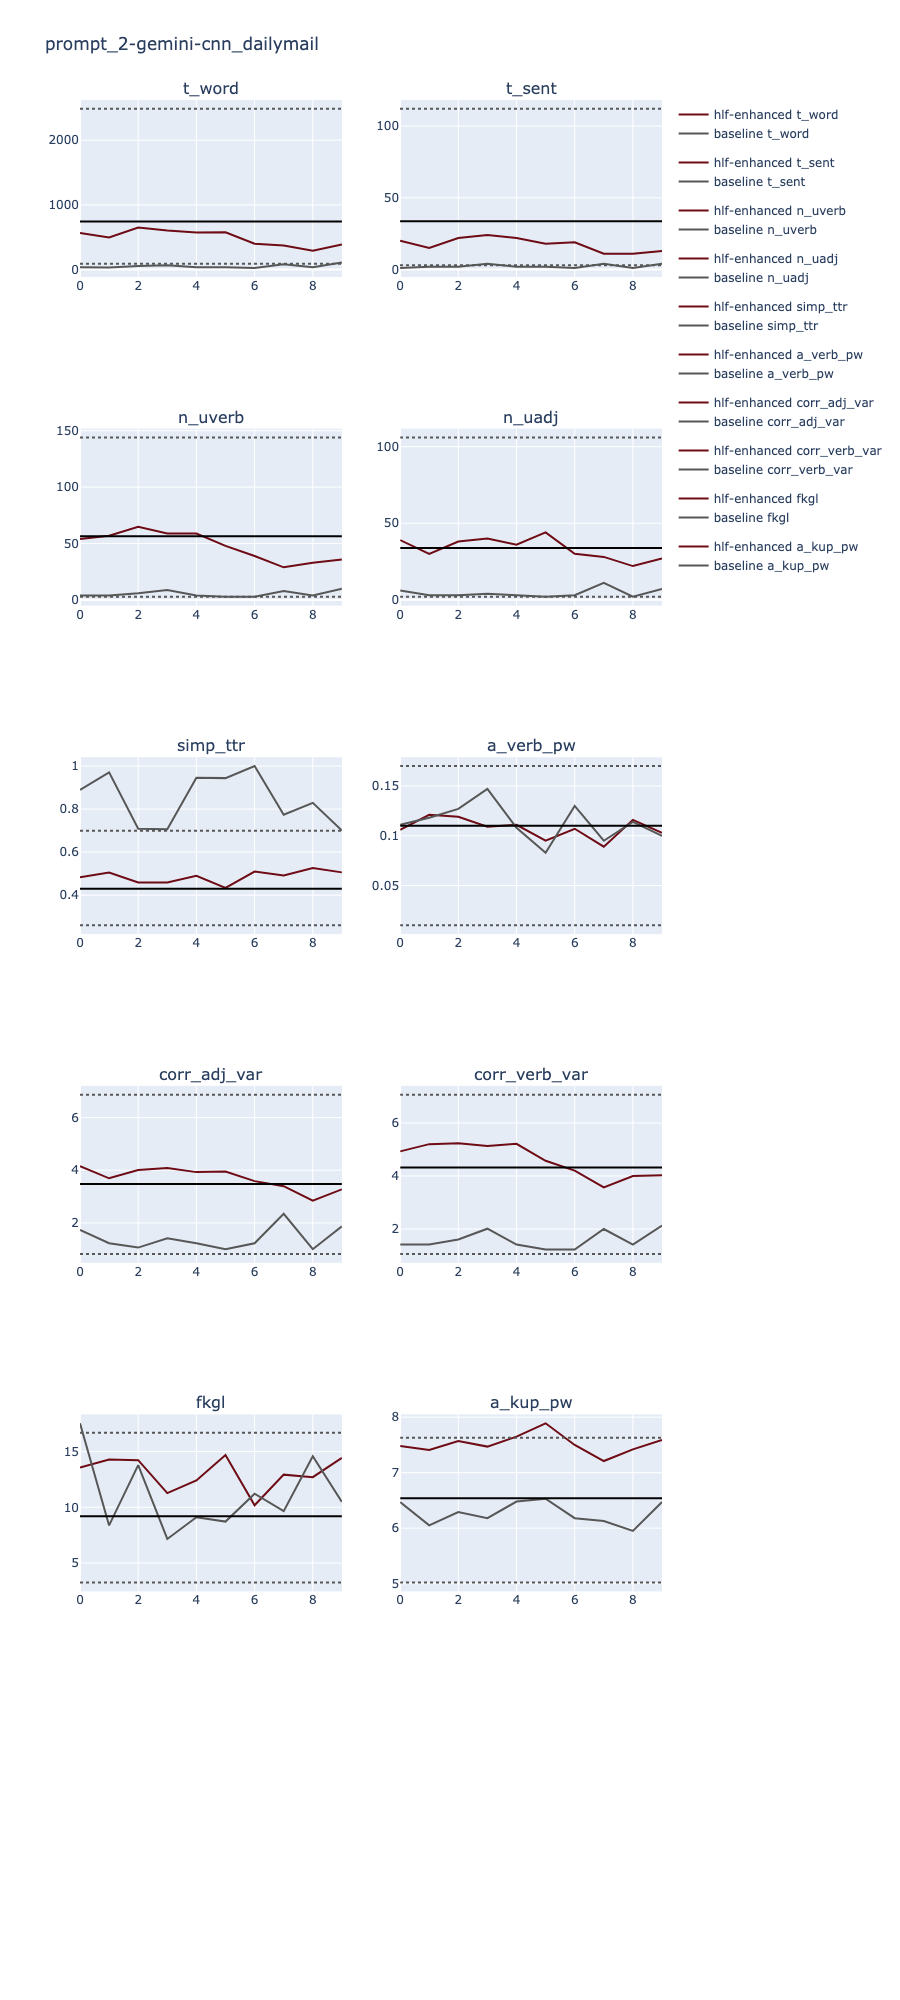
\includegraphics[width=\textwidth,height=0.9\textheight,scale=1]{plots/prompt_2_ifd/prompt_2-gemini-cnn_dailymail/prompt_2-gemini-cnn_dailymail.png}
    \caption{Gemini on CNN Corpus\\Prompt With Examples\\Input from Corpus}
    \label{fig:gemini-prompt2-cnn-ifd}
\end{figure*}
\begin{figure*}[ht]
    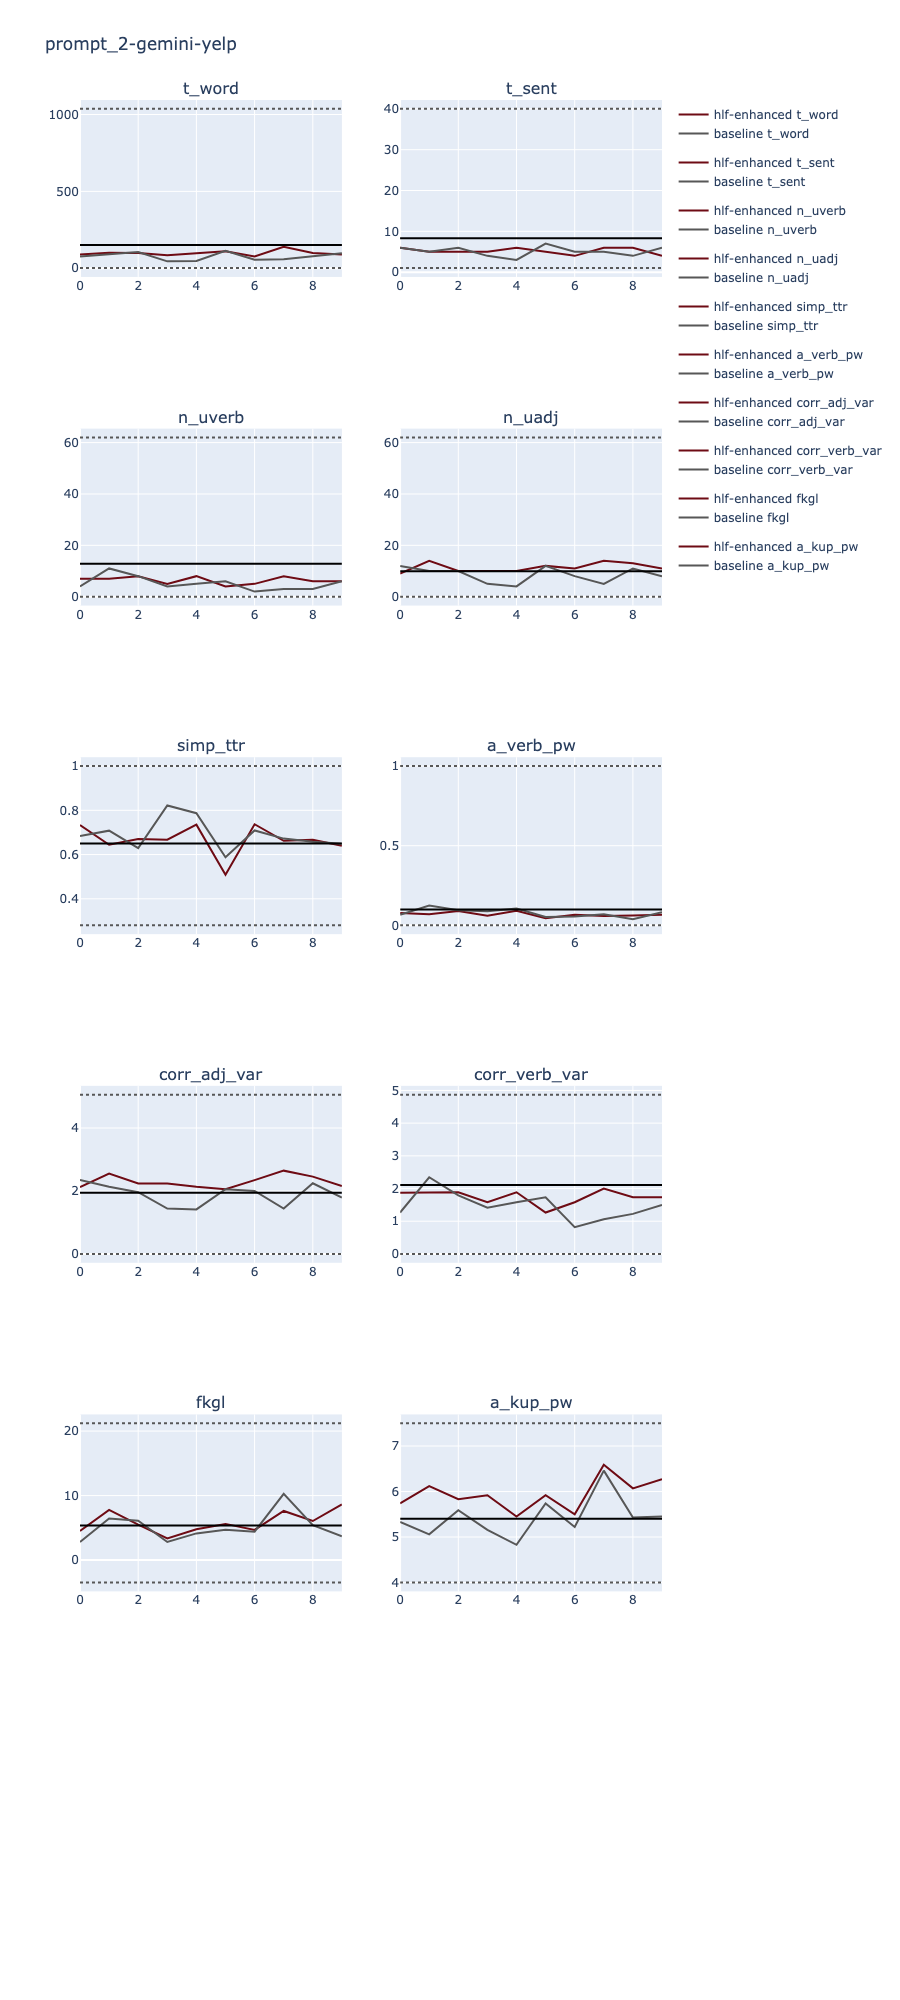
\includegraphics[width=\textwidth,height=0.9\textheight,scale=1]{plots/prompt_2_ifd/prompt_2-gemini-yelp/prompt_2-gemini-yelp.png}
    \caption{Gemini on Yelp Corpus\\Prompt With Examples\\Input from Corpus}
    \label{fig:gemini-prompt2-yelp-ifd}
\end{figure*}

\subsection{Claude3}

\Cref{fig:claude3-prompt1-cnn,fig:claude3-prompt1-yelp,fig:claude3-prompt2-cnn,fig:claude3-prompt2-yelp,fig:claude3-prompt2-cnn-ifd,fig:claude3-prompt2-yelp-ifd}
show the experiment results for the Claude 3 Opus large language model.

\begin{figure*}[ht]
    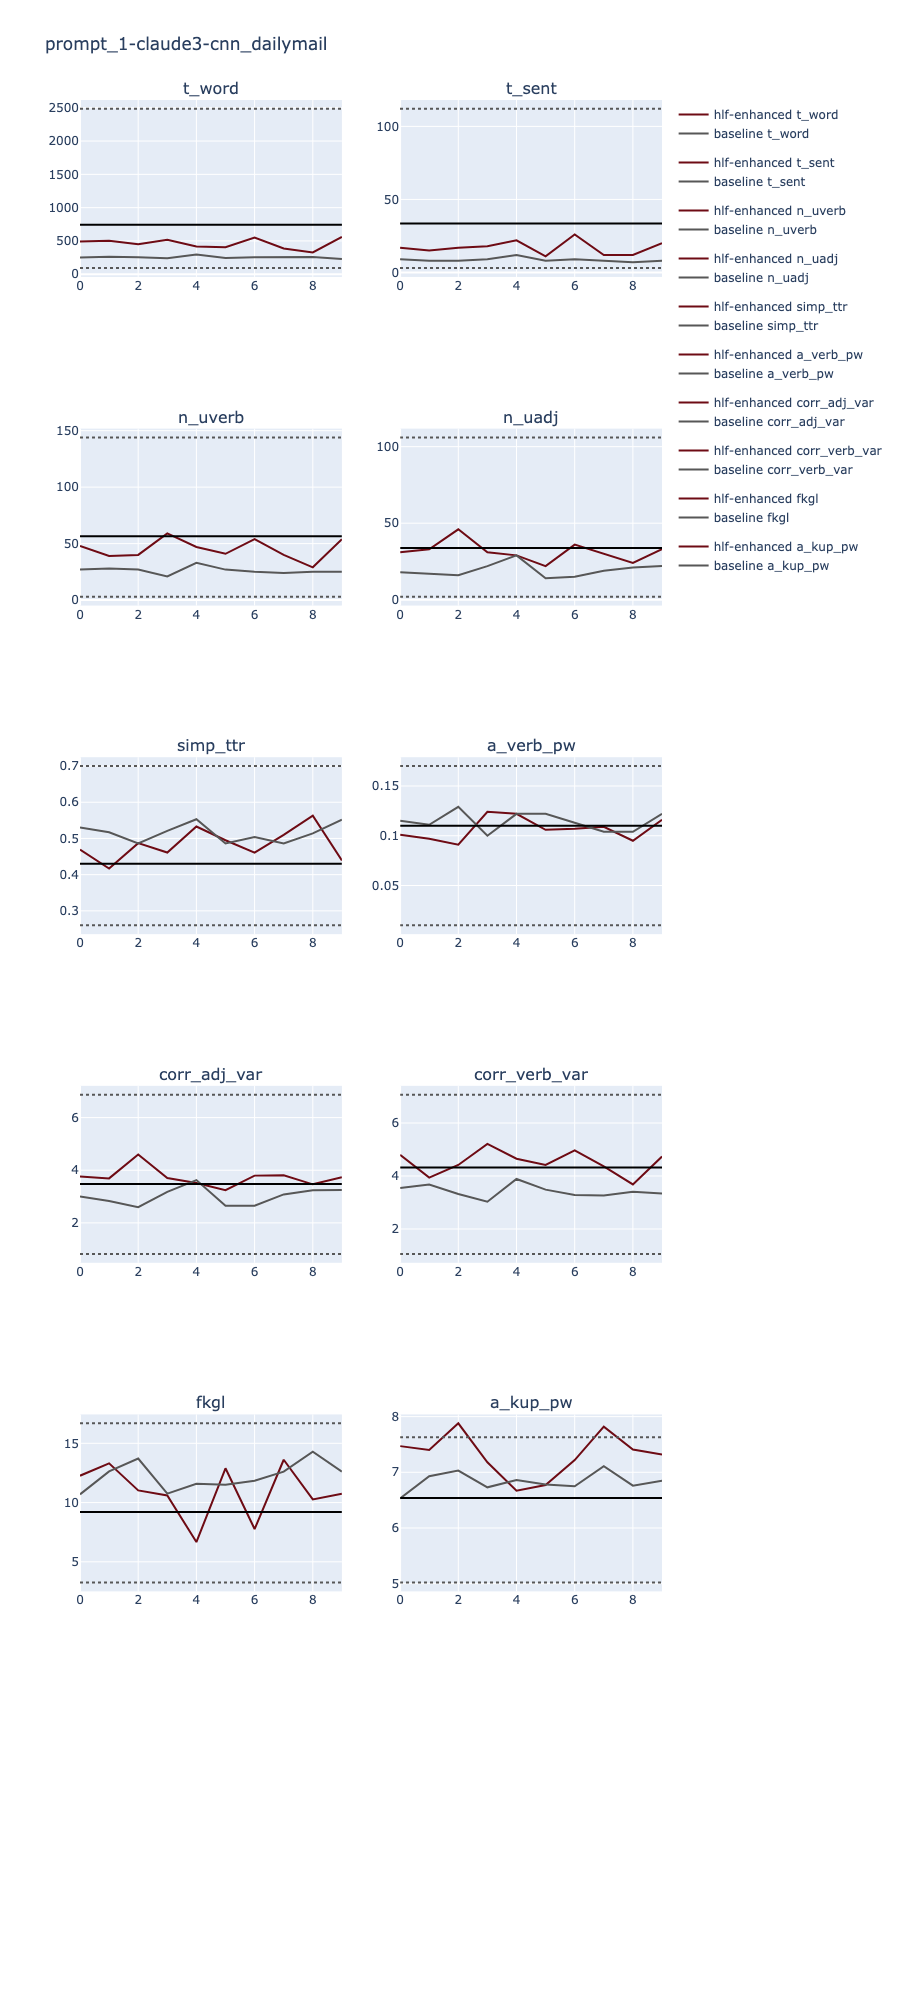
\includegraphics[width=\textwidth,height=0.9\textheight,scale=1]{plots/prompt_1/prompt_1-claude3-cnn_dailymail/prompt_1-claude3-cnn_dailymail.png}
    \caption{Claude3 on CNN Corpus\\Prompt Without Examples}
    \label{fig:claude3-prompt1-cnn}
\end{figure*}
\begin{figure*}[ht]
    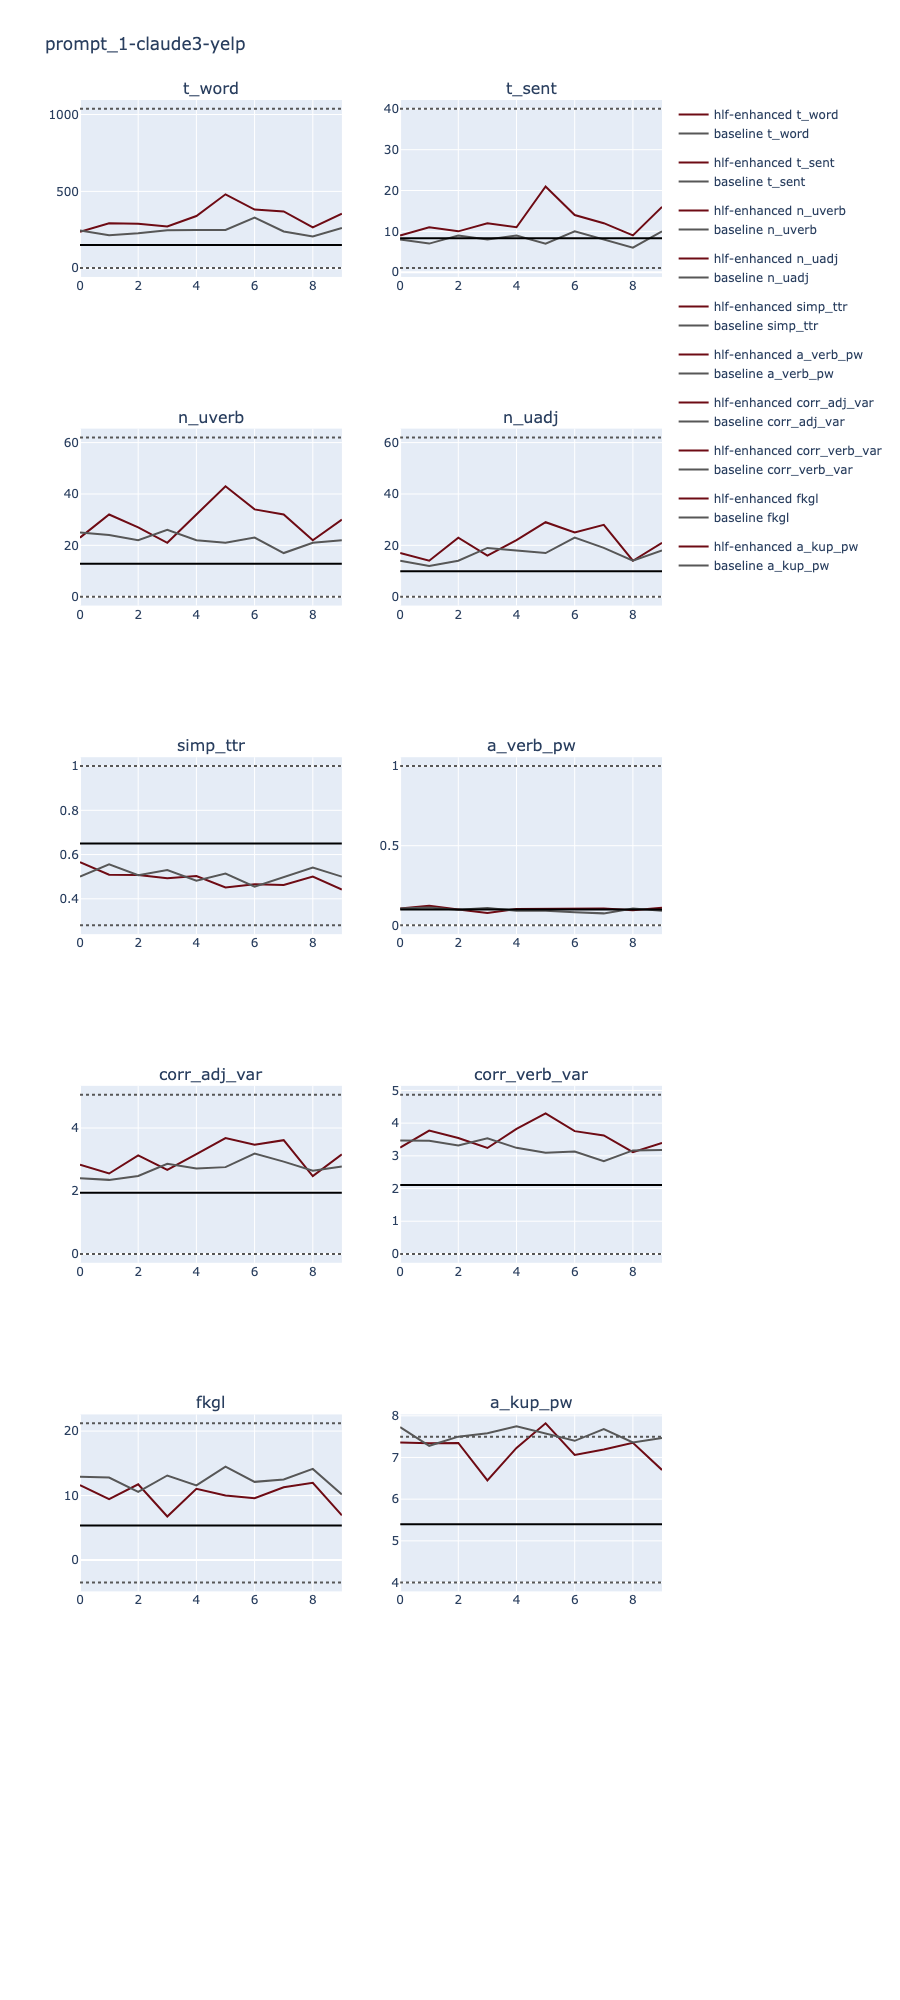
\includegraphics[width=\textwidth,height=0.9\textheight,scale=1]{plots/prompt_1/prompt_1-claude3-yelp/prompt_1-claude3-yelp.png}
    \caption{Claude3 on Yelp Corpus\\Prompt Without Examples}
    \label{fig:claude3-prompt1-yelp}
\end{figure*}
\begin{figure*}[ht]
    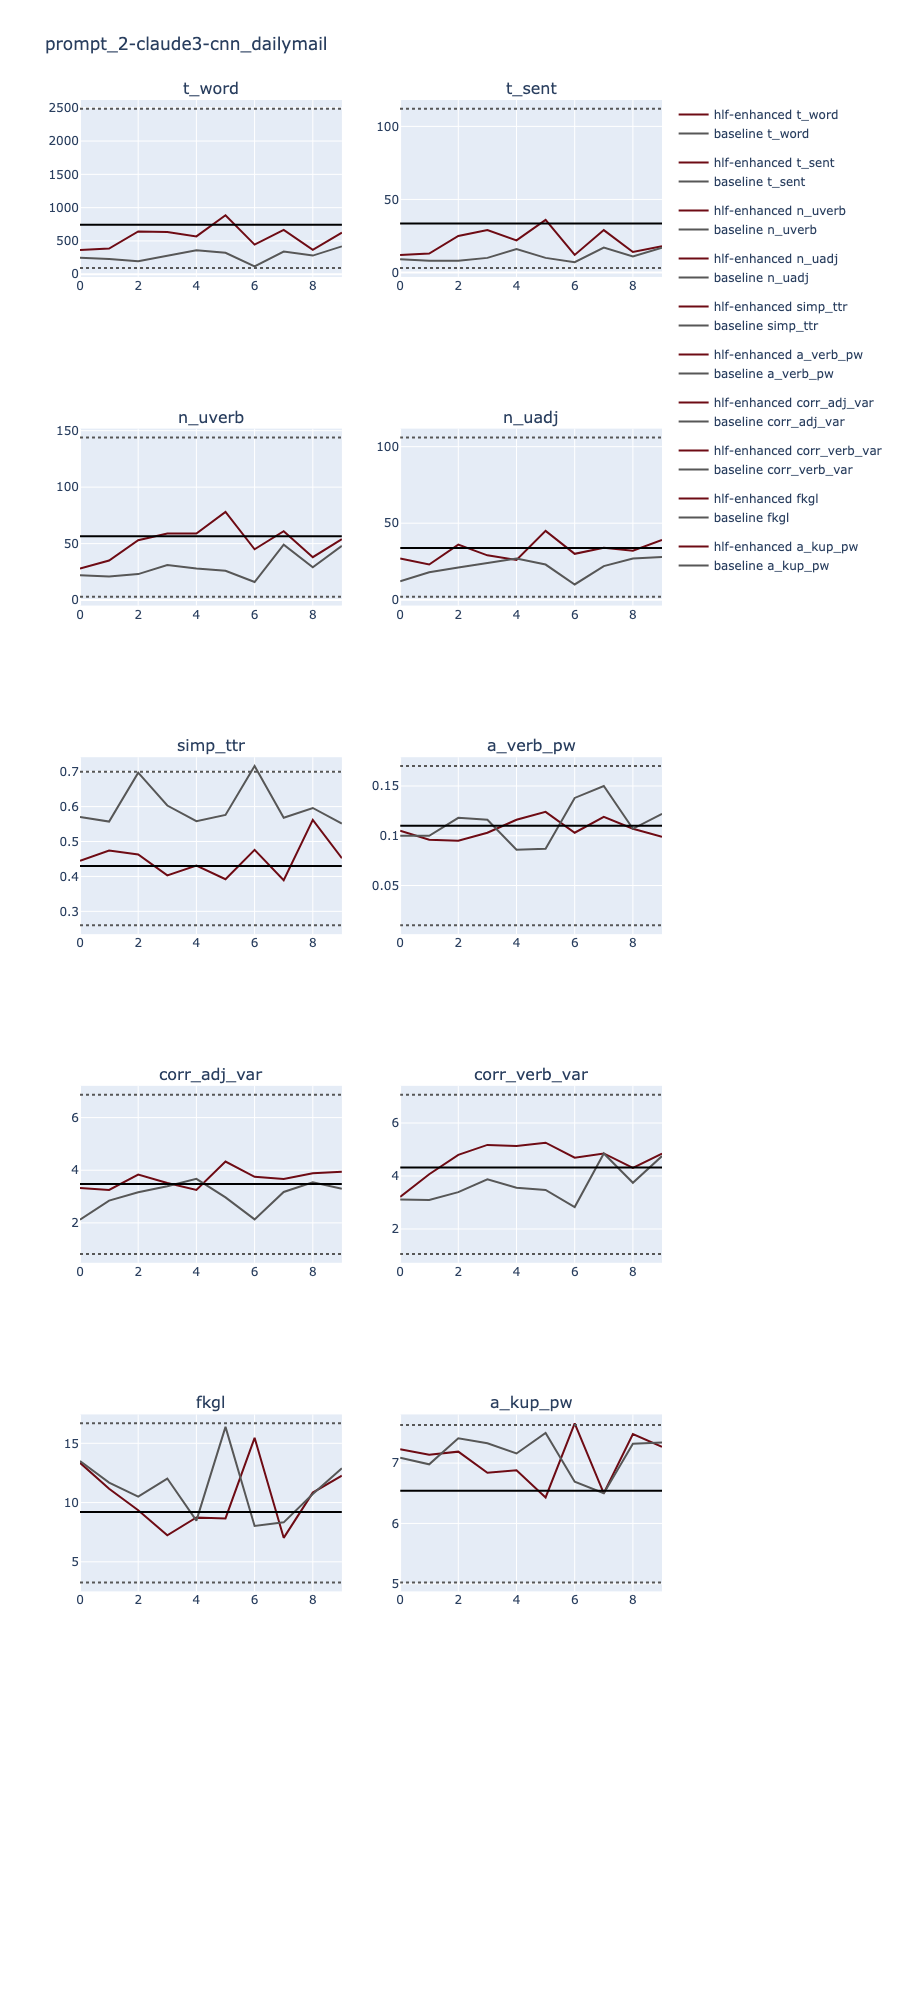
\includegraphics[width=\textwidth,height=0.9\textheight,scale=1]{plots/prompt_2/prompt_2-claude3-cnn_dailymail/prompt_2-claude3-cnn_dailymail.png}
    \caption{Claude3 on CNN Corpus\\Prompt With Examples\\Extraneous Input}
    \label{fig:claude3-prompt2-cnn}
\end{figure*}
\begin{figure*}[ht]
    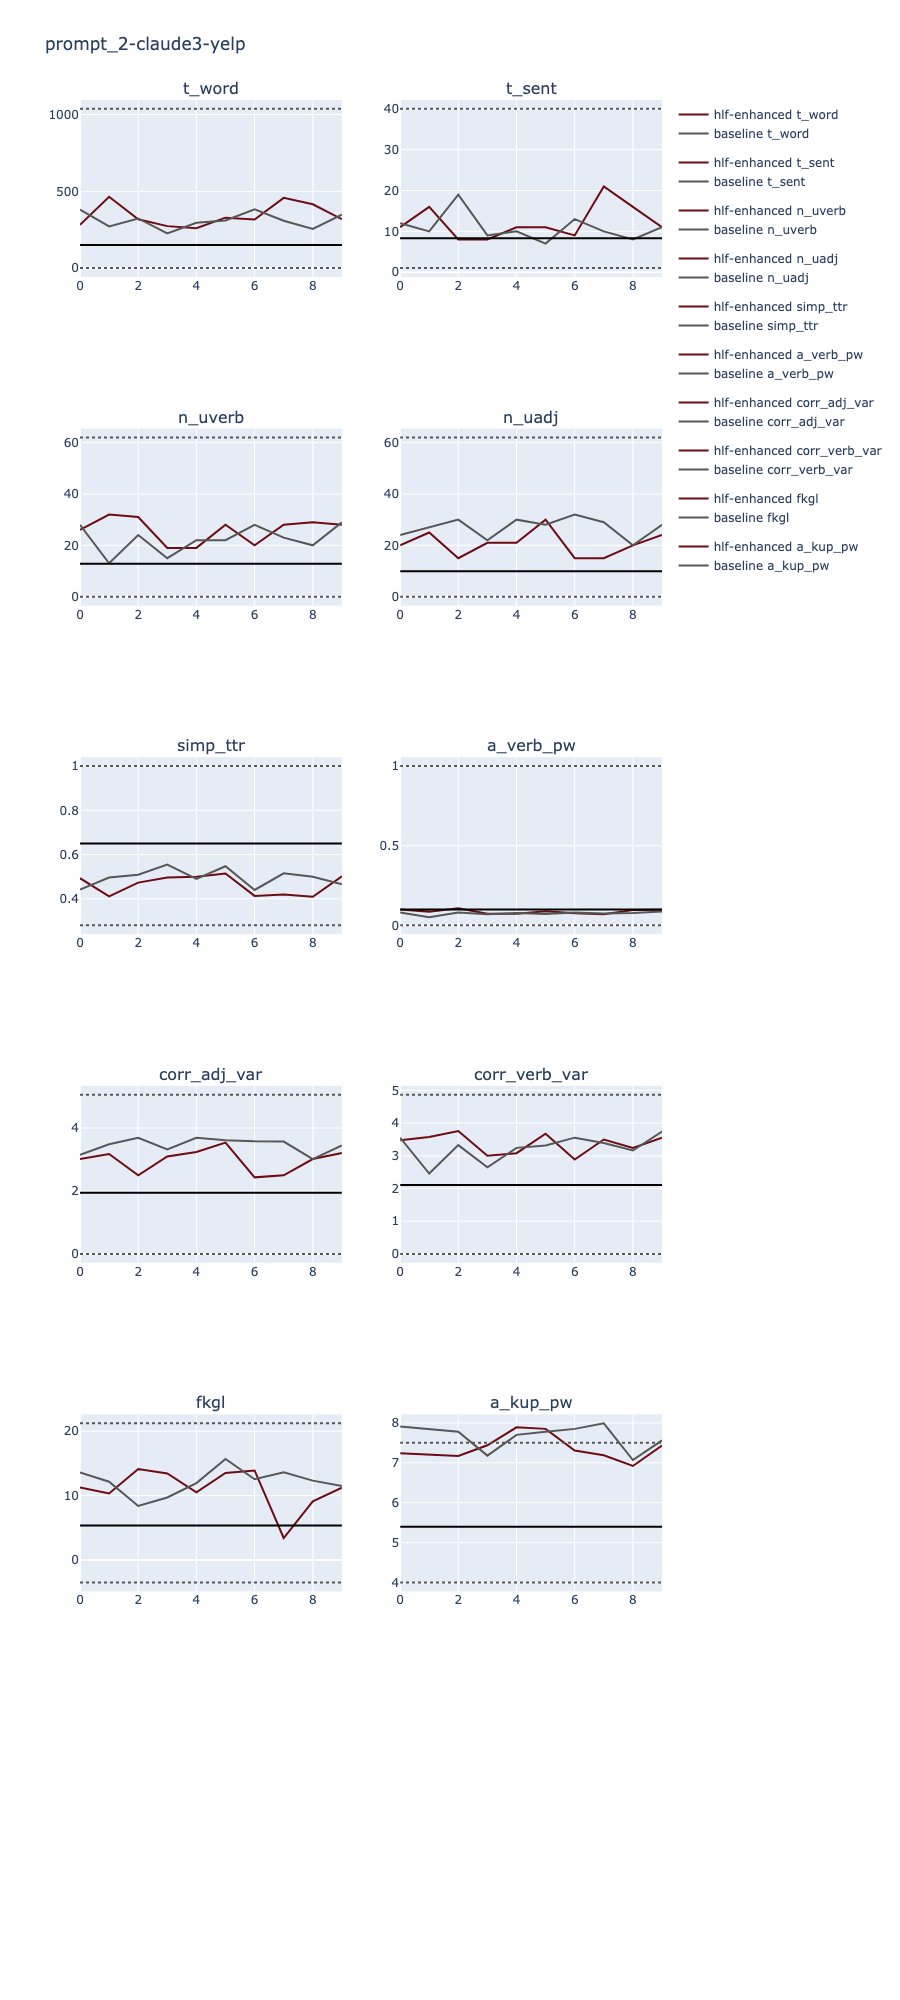
\includegraphics[width=\textwidth,height=0.9\textheight,scale=1]{plots/prompt_2/prompt_2-claude3-yelp/prompt_2-claude3-yelp.png}
    \caption{Claude3 on Yelp Corpus\\Prompt With Examples\\Extraneous Input}
    \label{fig:claude3-prompt2-yelp}
\end{figure*}
\begin{figure*}[ht]
    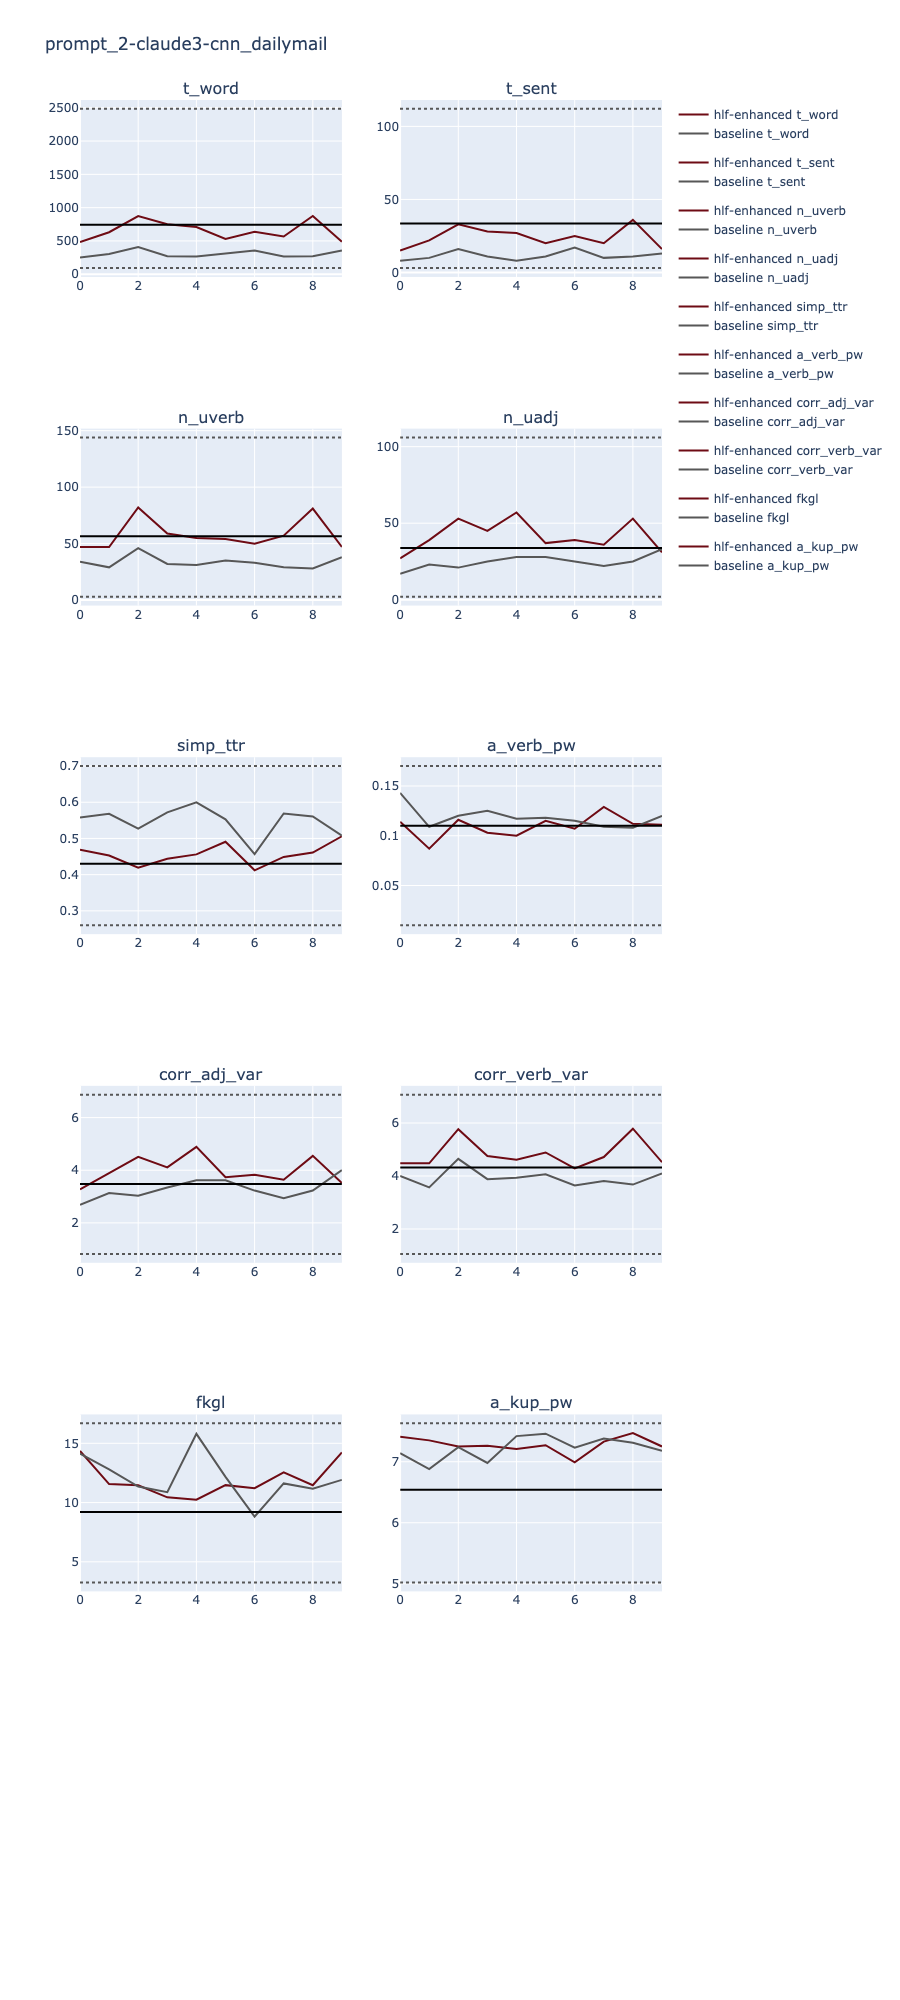
\includegraphics[width=\textwidth,height=0.9\textheight,scale=1]{plots/prompt_2_ifd/prompt_2-claude3-cnn_dailymail/prompt_2-claude3-cnn_dailymail.png}
    \caption{Claude3 on CNN Corpus\\Prompt With Examples\\Input from Corpus}
    \label{fig:claude3-prompt2-cnn-ifd}
\end{figure*}
\begin{figure*}[ht]
    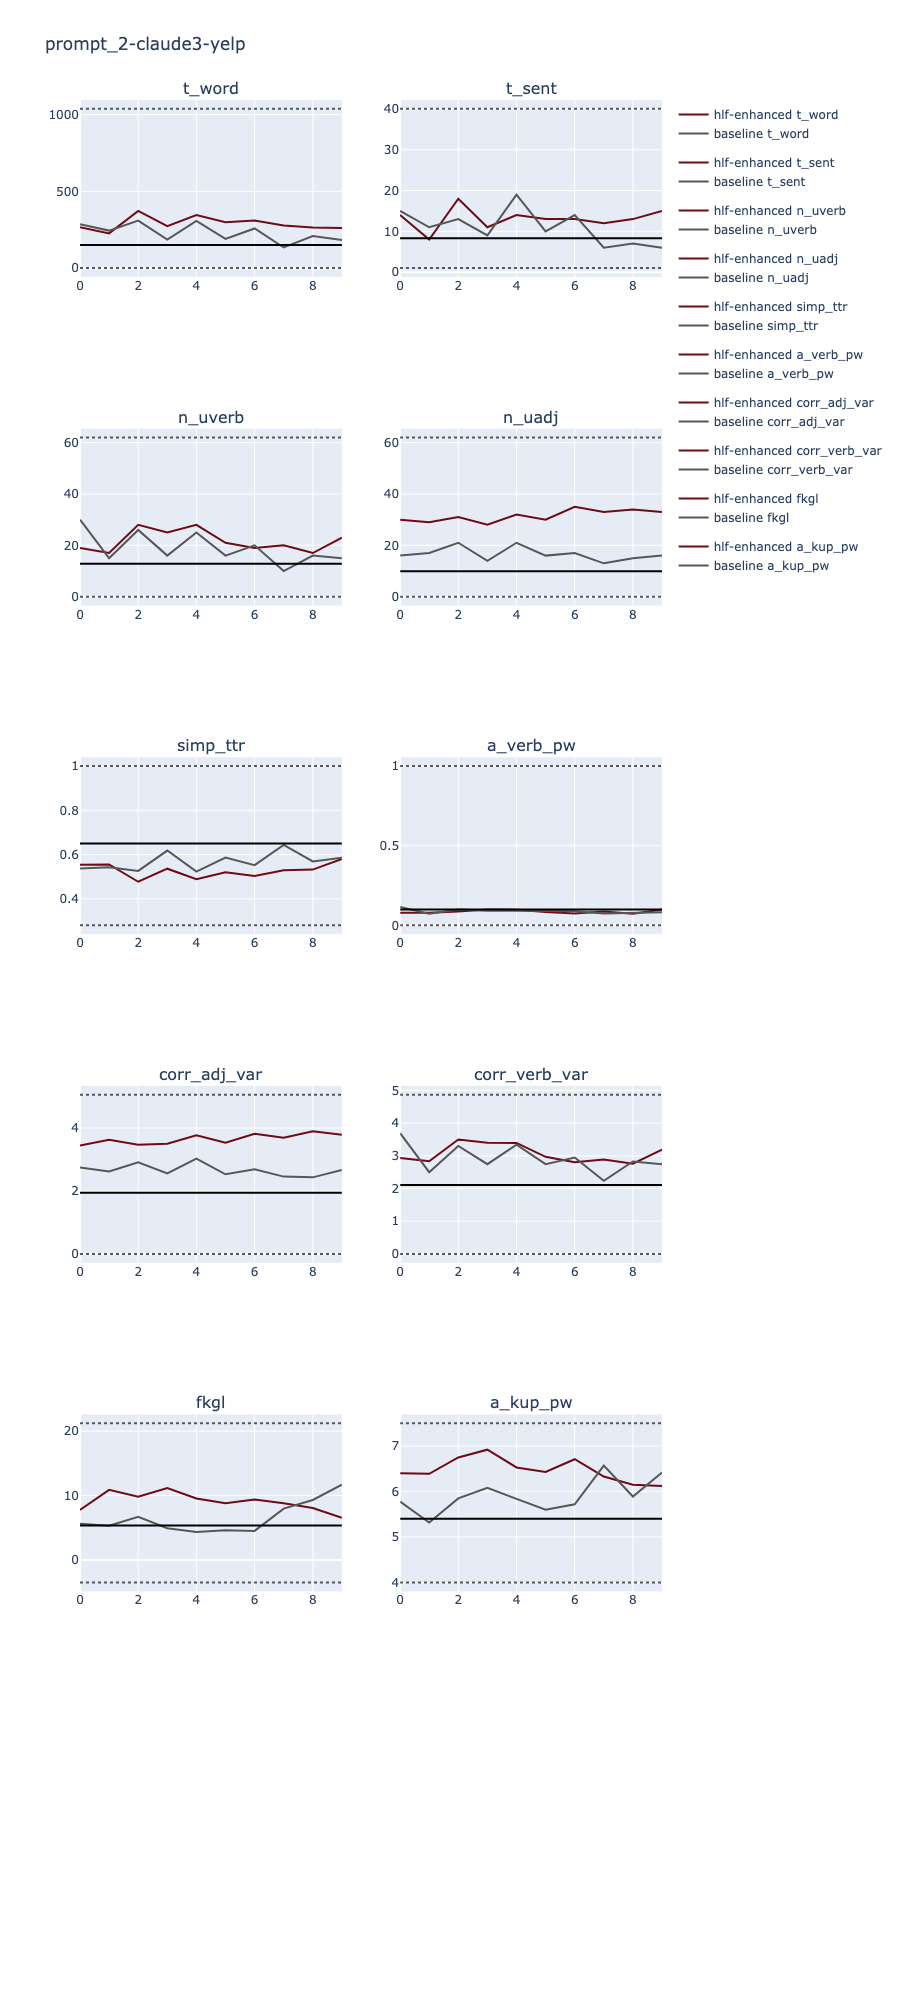
\includegraphics[width=\textwidth,height=0.9\textheight,scale=1]{plots/prompt_2_ifd/prompt_2-claude3-yelp/prompt_2-claude3-yelp.png}
    \caption{Claude3 on Yelp Corpus\\Prompt With Examples\\Input from Corpus}
    \label{fig:claude3-prompt2-yelp-ifd}
\end{figure*}

\subsection{Llama3}

\Cref{fig:llama3_70b-prompt1-cnn,fig:llama3_70b-prompt1-yelp,fig:llama3_70b-prompt2-cnn,fig:llama3_70b-prompt2-yelp,fig:llama3_70b-prompt2-cnn-ifd,fig:llama3_70b-prompt2-yelp-ifd}
show the experiment results for the Claude 3 Opus large language model.

\begin{figure*}[ht]
    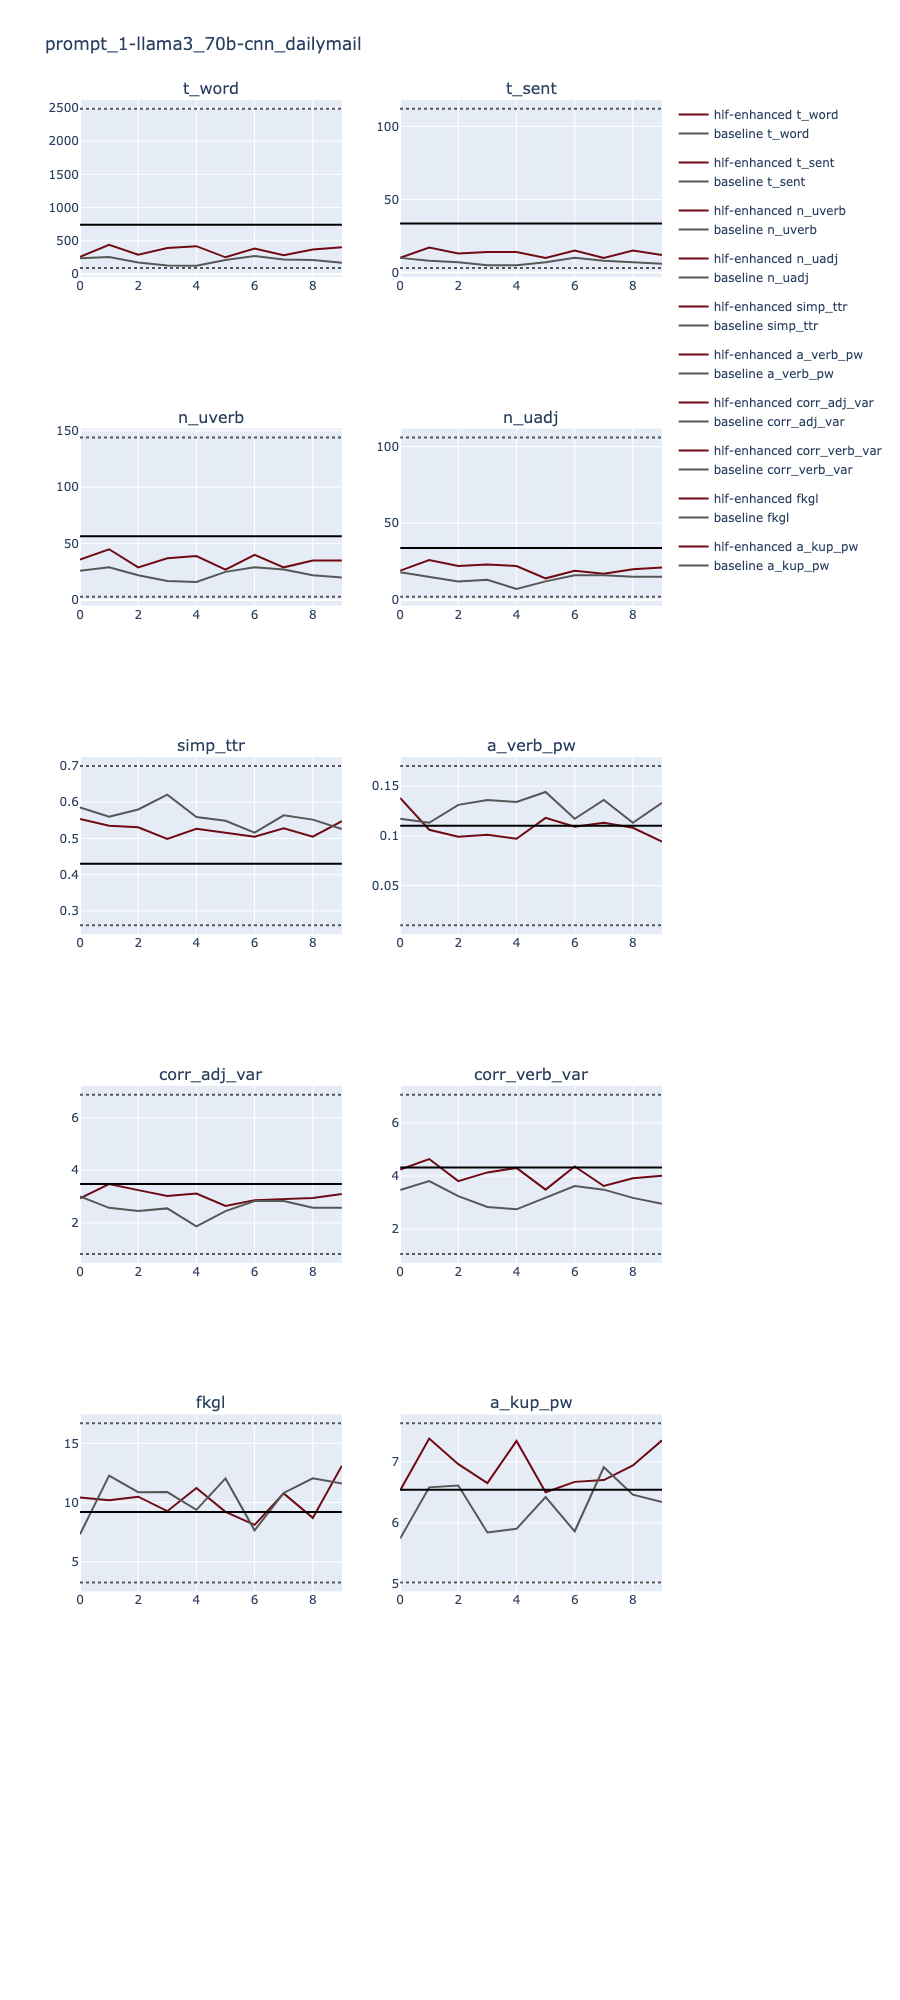
\includegraphics[width=\textwidth,height=0.9\textheight,scale=1]{plots/prompt_1/prompt_1-llama3_70b-cnn_dailymail/prompt_1-llama3_70b-cnn_dailymail.png}
    \caption{Llama3 on CNN Corpus\\Prompt Without Examples}
    \label{fig:llama3_70b-prompt1-cnn}
\end{figure*}
\begin{figure*}[ht]
    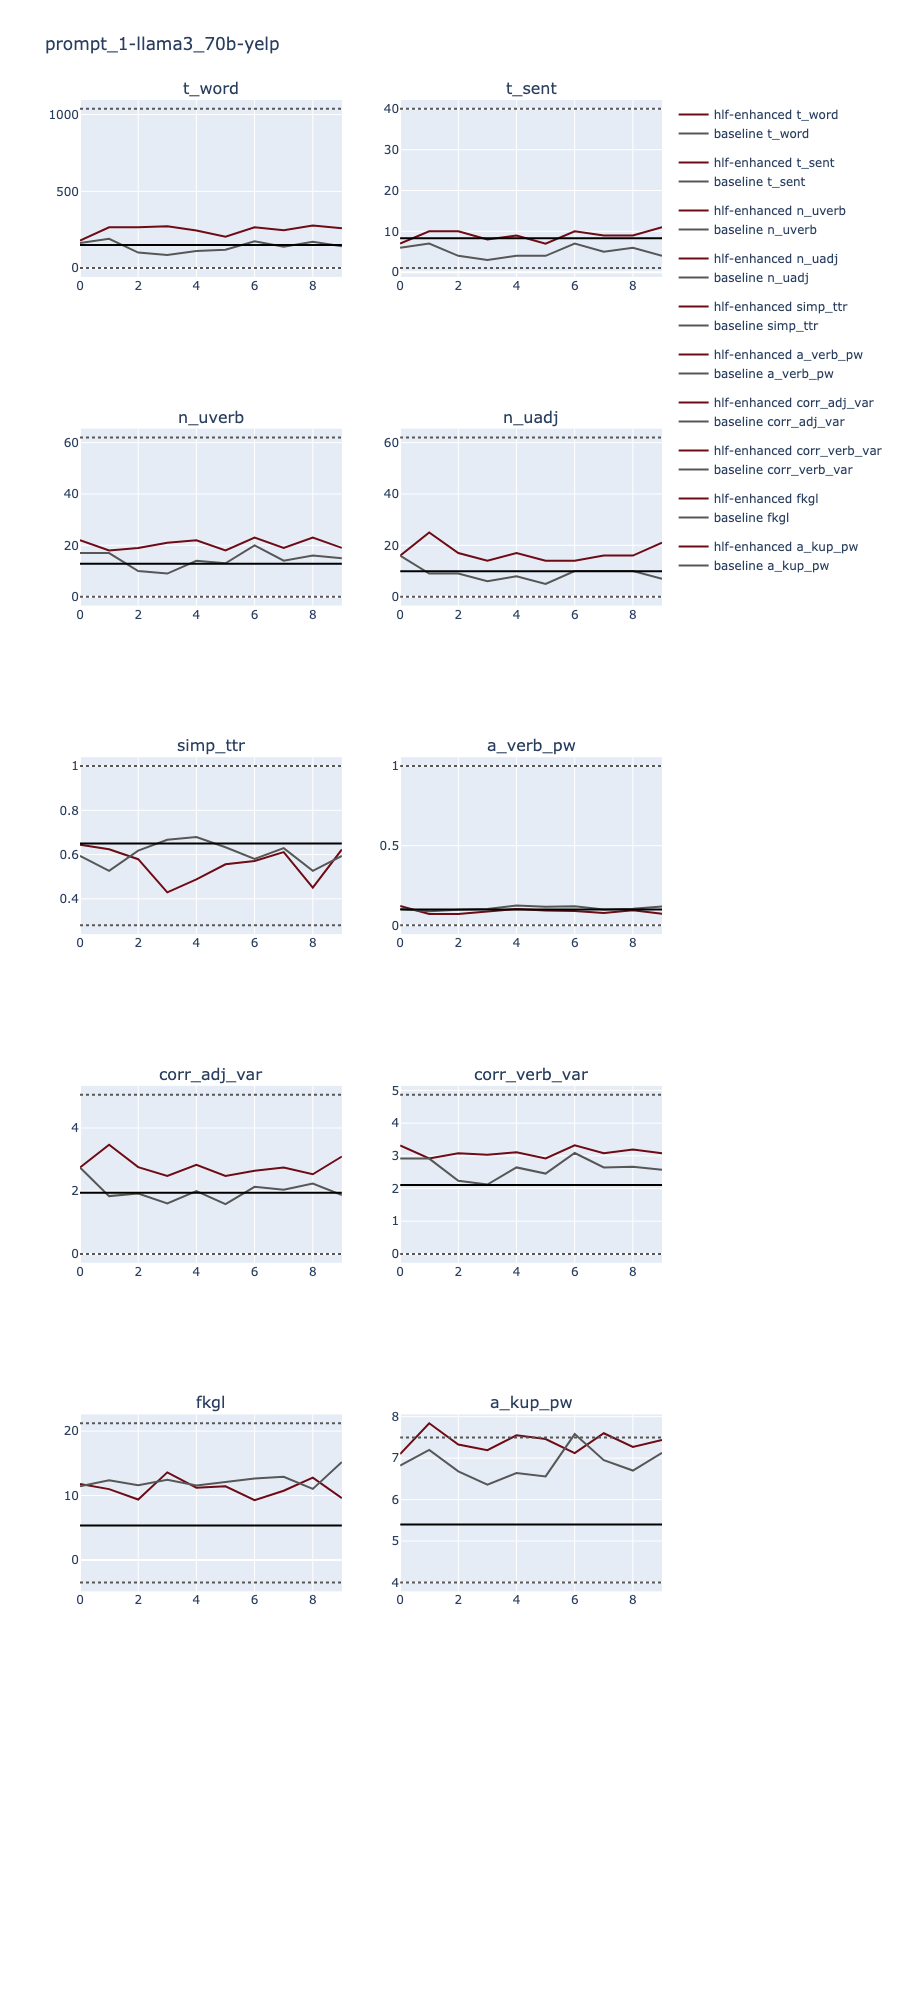
\includegraphics[width=\textwidth,height=0.9\textheight,scale=1]{plots/prompt_1/prompt_1-llama3_70b-yelp/prompt_1-llama3_70b-yelp.png}
    \caption{Llama3 on Yelp Corpus\\Prompt Without Examples}
    \label{fig:llama3_70b-prompt1-yelp}
\end{figure*}
\begin{figure*}[ht]
    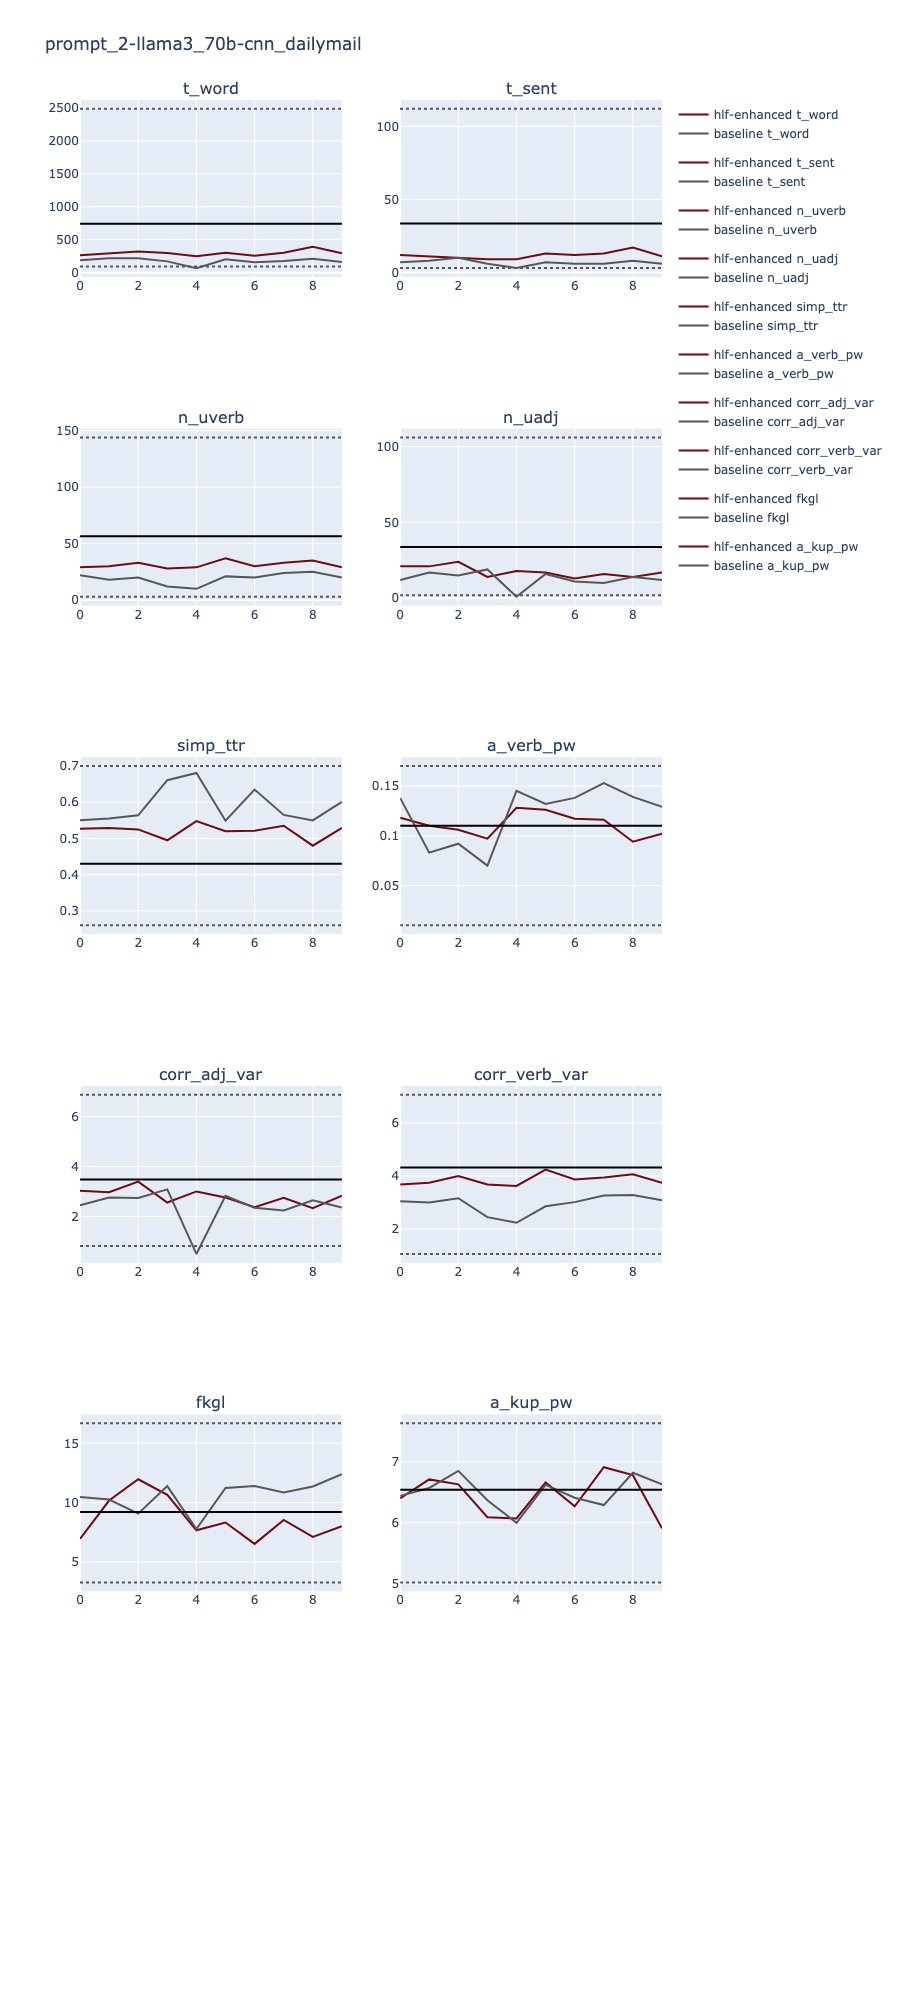
\includegraphics[width=\textwidth,height=0.9\textheight,scale=1]{plots/prompt_2/prompt_2-llama3_70b-cnn_dailymail/prompt_2-llama3_70b-cnn_dailymail.png}
    \caption{Llama3 on CNN Corpus\\Prompt With Examples\\Extraneous Input}
    \label{fig:llama3_70b-prompt2-cnn}
\end{figure*}
\begin{figure*}[ht]
    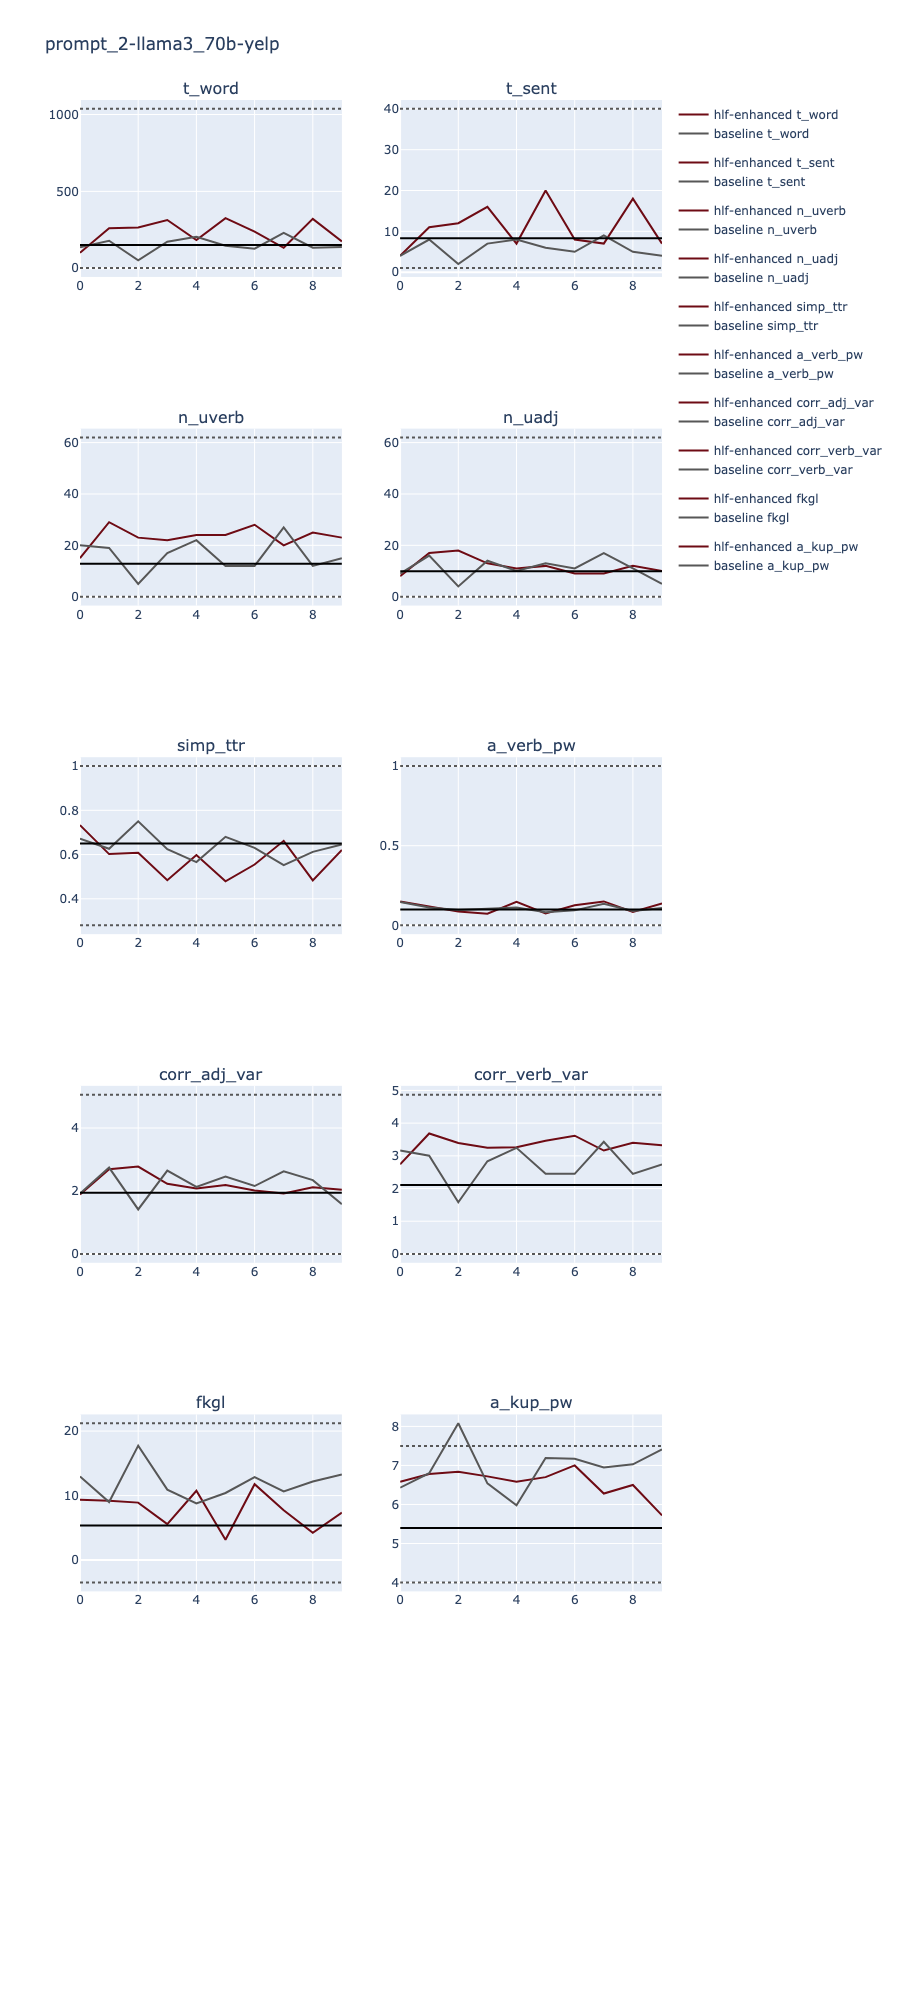
\includegraphics[width=\textwidth,height=0.9\textheight,scale=1]{plots/prompt_2/prompt_2-llama3_70b-yelp/prompt_2-llama3_70b-yelp.png}
    \caption{Llama3 on Yelp Corpus\\Prompt With Examples\\Extraneous Input}
    \label{fig:llama3_70b-prompt2-yelp}
\end{figure*}
\begin{figure*}[ht]
    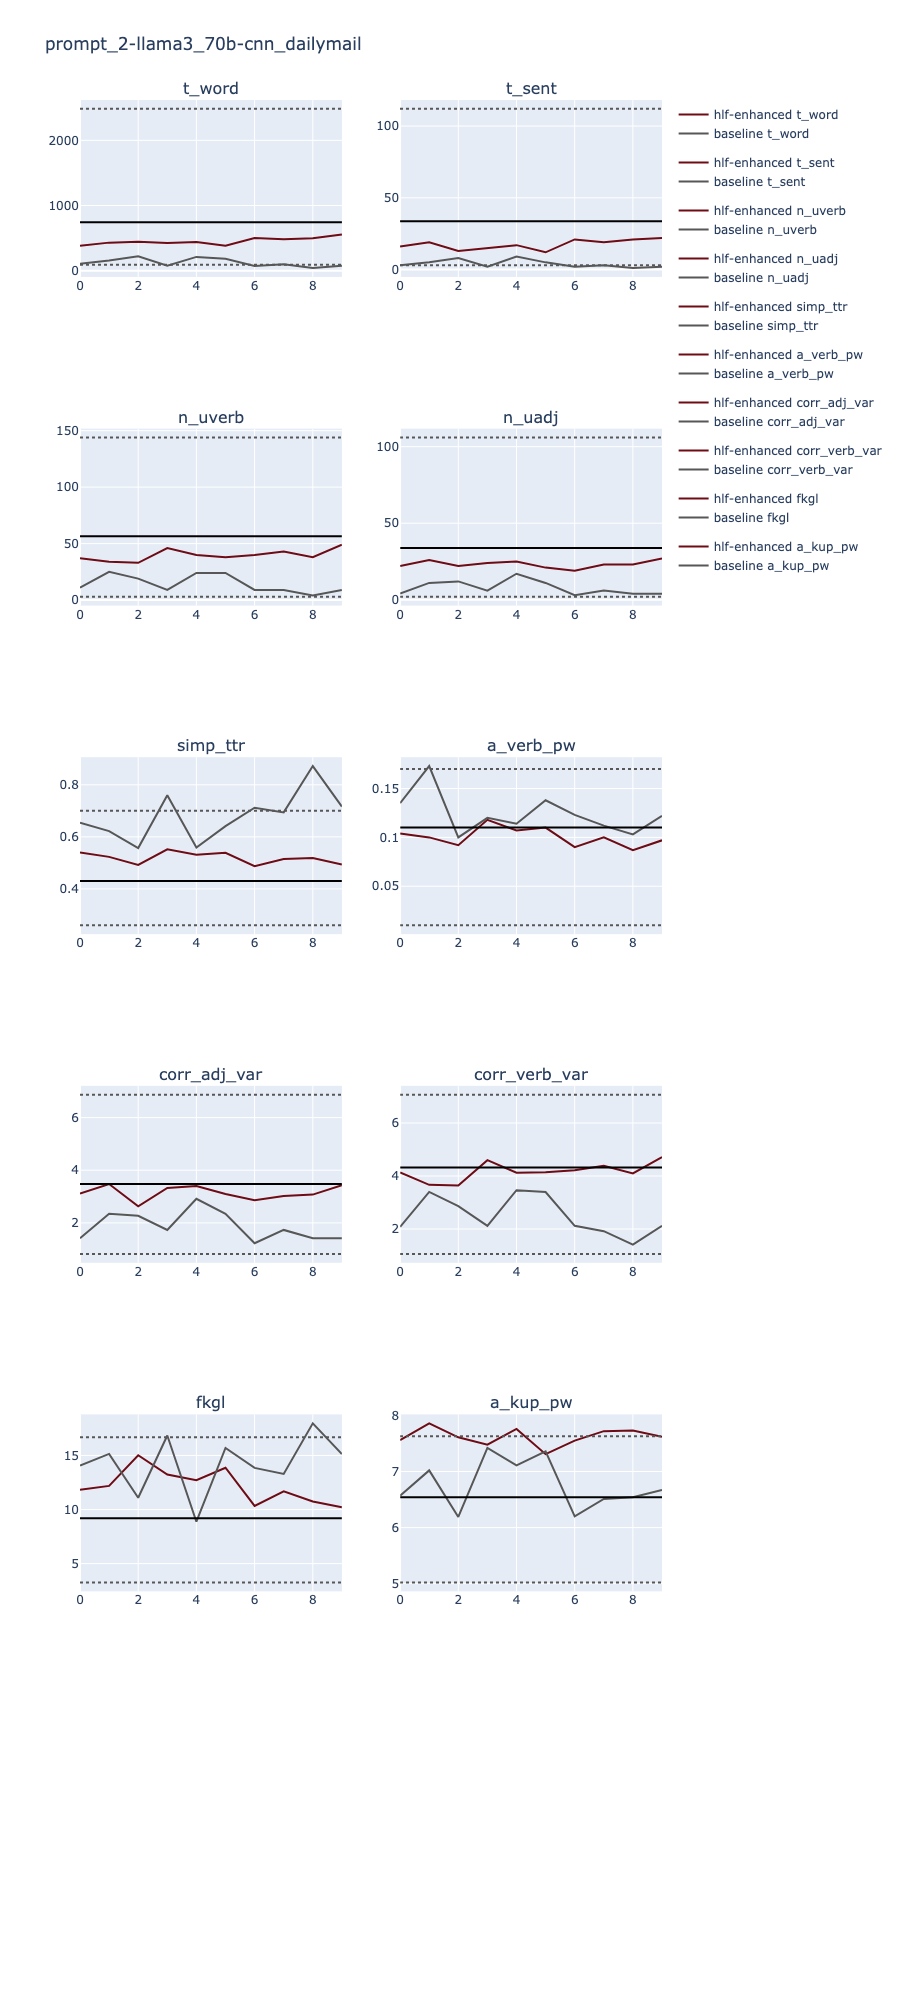
\includegraphics[width=\textwidth,height=0.9\textheight,scale=1]{plots/prompt_2_ifd/prompt_2-llama3_70b-cnn_dailymail/prompt_2-llama3_70b-cnn_dailymail.png}
    \caption{Llama3 on CNN Corpus\\Prompt With Examples\\Input from Corpus}
    \label{fig:llama3_70b-prompt2-cnn-ifd}
\end{figure*}
\begin{figure*}[ht]
    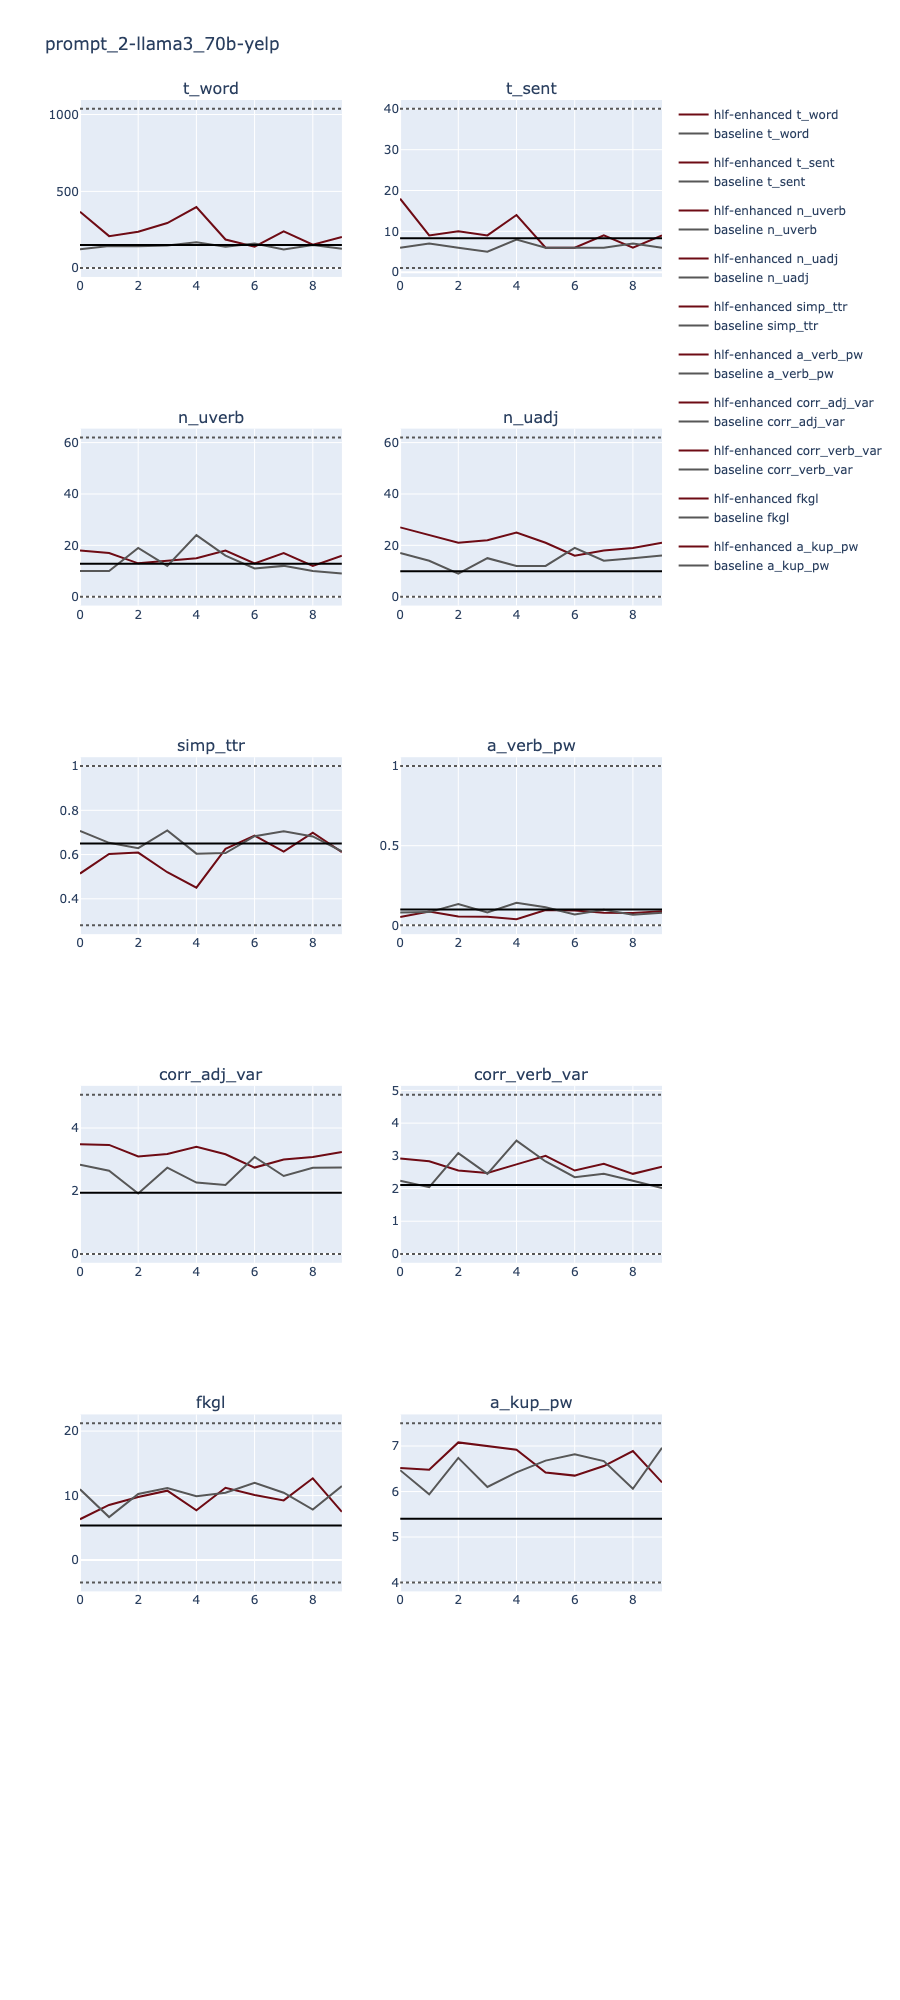
\includegraphics[width=\textwidth,height=0.9\textheight,scale=1]{plots/prompt_2_ifd/prompt_2-llama3_70b-yelp/prompt_2-llama3_70b-yelp.png}
    \caption{Llama3 on Yelp Corpus\\Prompt With Examples\\Input from Corpus}
    \label{fig:llama3_70b-prompt2-yelp-ifd}
\end{figure*}

\subsection{Command R+}

\Cref{fig:command_r-prompt1-cnn,fig:command_r-prompt1-yelp,fig:command_r-prompt2-cnn,fig:command_r-prompt2-yelp,fig:command_r-prompt2-cnn-ifd,fig:command_r-prompt2-yelp-ifd}
show the experiment results for the Claude 3 Opus large language model.

\begin{figure*}[ht]
    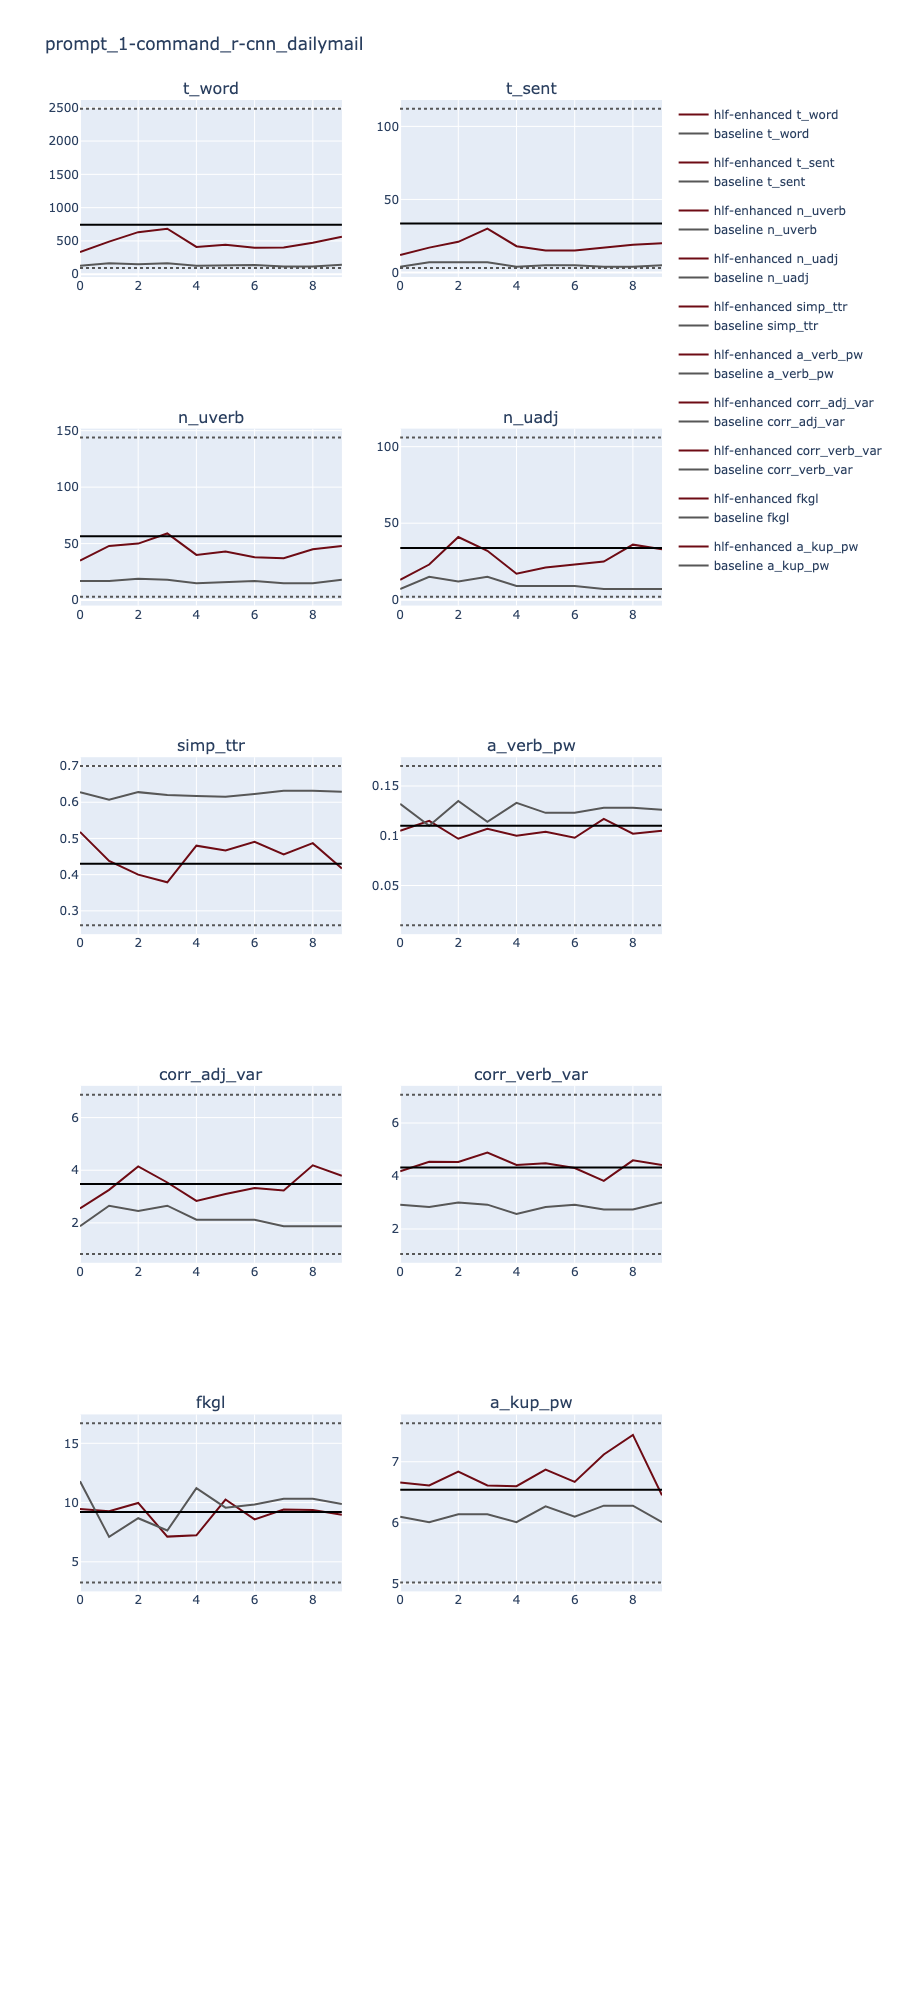
\includegraphics[width=\textwidth,height=0.9\textheight,scale=1]{plots/prompt_1/prompt_1-command_r-cnn_dailymail/prompt_1-command_r-cnn_dailymail.png}
    \caption{Command R on CNN Corpus\\Prompt Without Examples}
    \label{fig:command_r-prompt1-cnn}
\end{figure*}
\begin{figure*}[ht]
    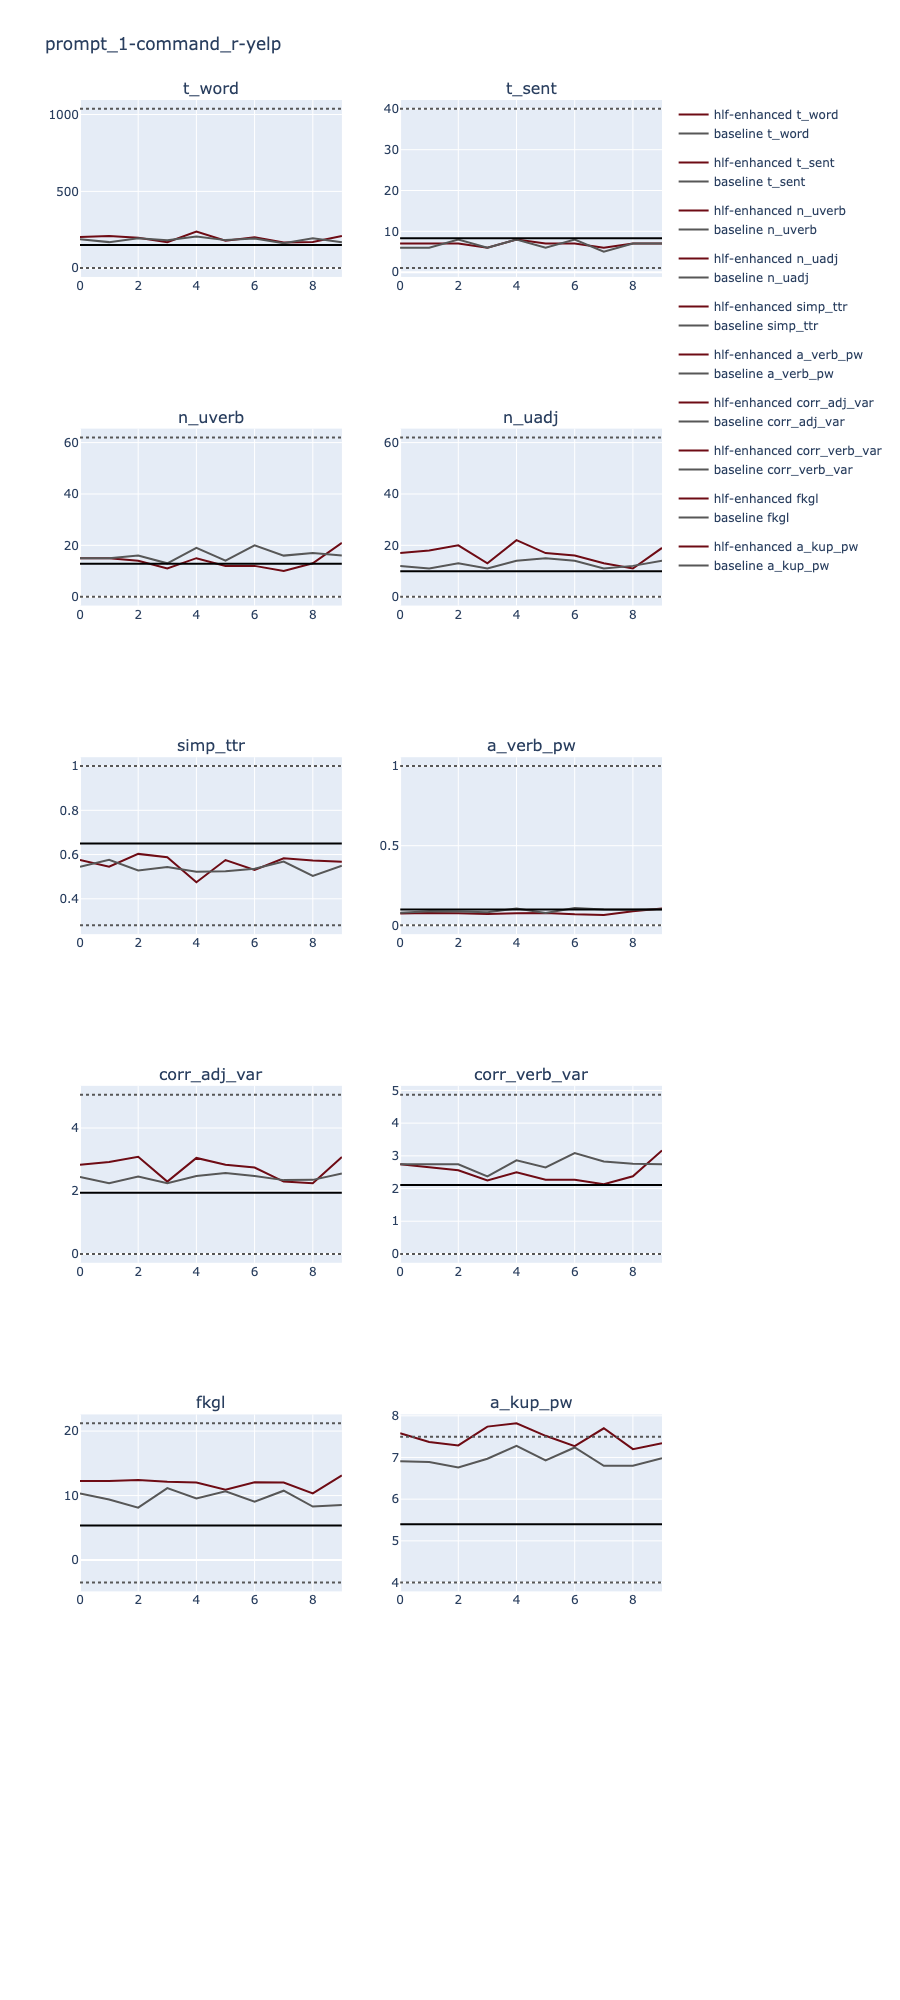
\includegraphics[width=\textwidth,height=0.9\textheight,scale=1]{plots/prompt_1/prompt_1-command_r-yelp/prompt_1-command_r-yelp.png}
    \caption{Command R on Yelp Corpus\\Prompt Without Examples}
    \label{fig:command_r-prompt1-yelp}
\end{figure*}
\begin{figure*}[ht]
    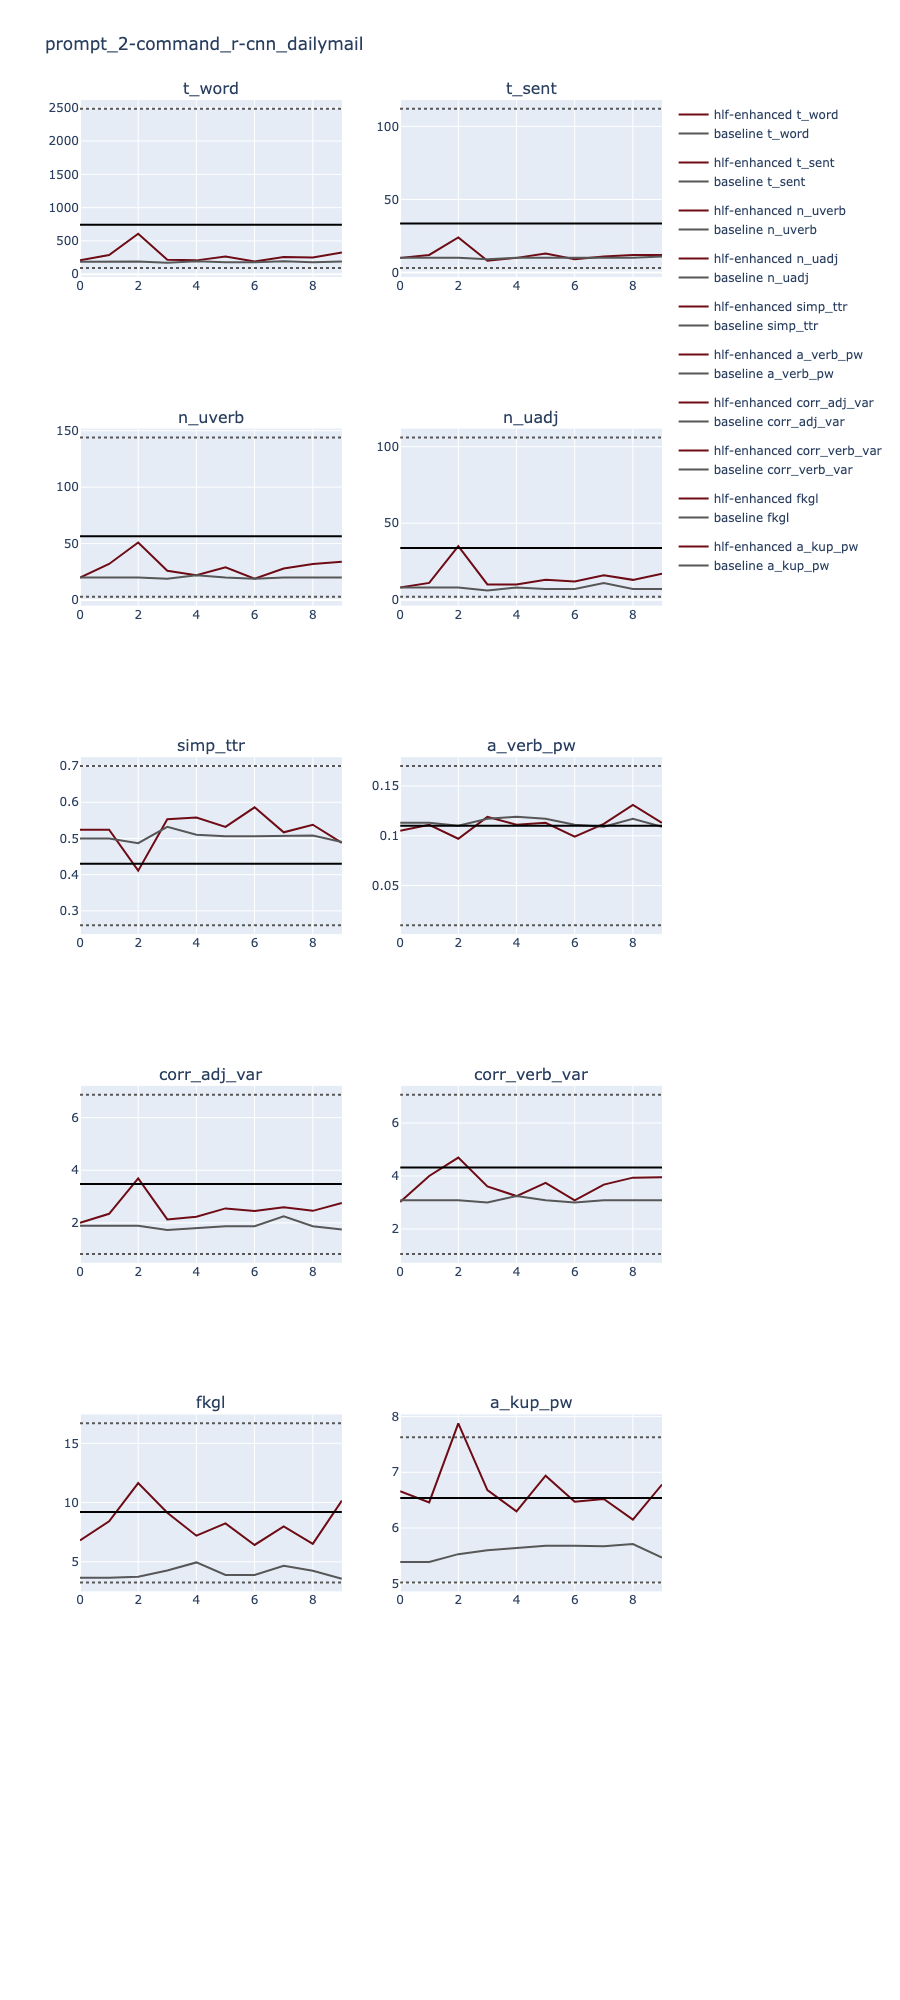
\includegraphics[width=\textwidth,height=0.9\textheight,scale=1]{plots/prompt_2/prompt_2-command_r-cnn_dailymail/prompt_2-command_r-cnn_dailymail.png}
    \caption{Command R on CNN Corpus\\Prompt With Examples\\Extraneous Input}
    \label{fig:command_r-prompt2-cnn}
\end{figure*}
\begin{figure*}[ht]
    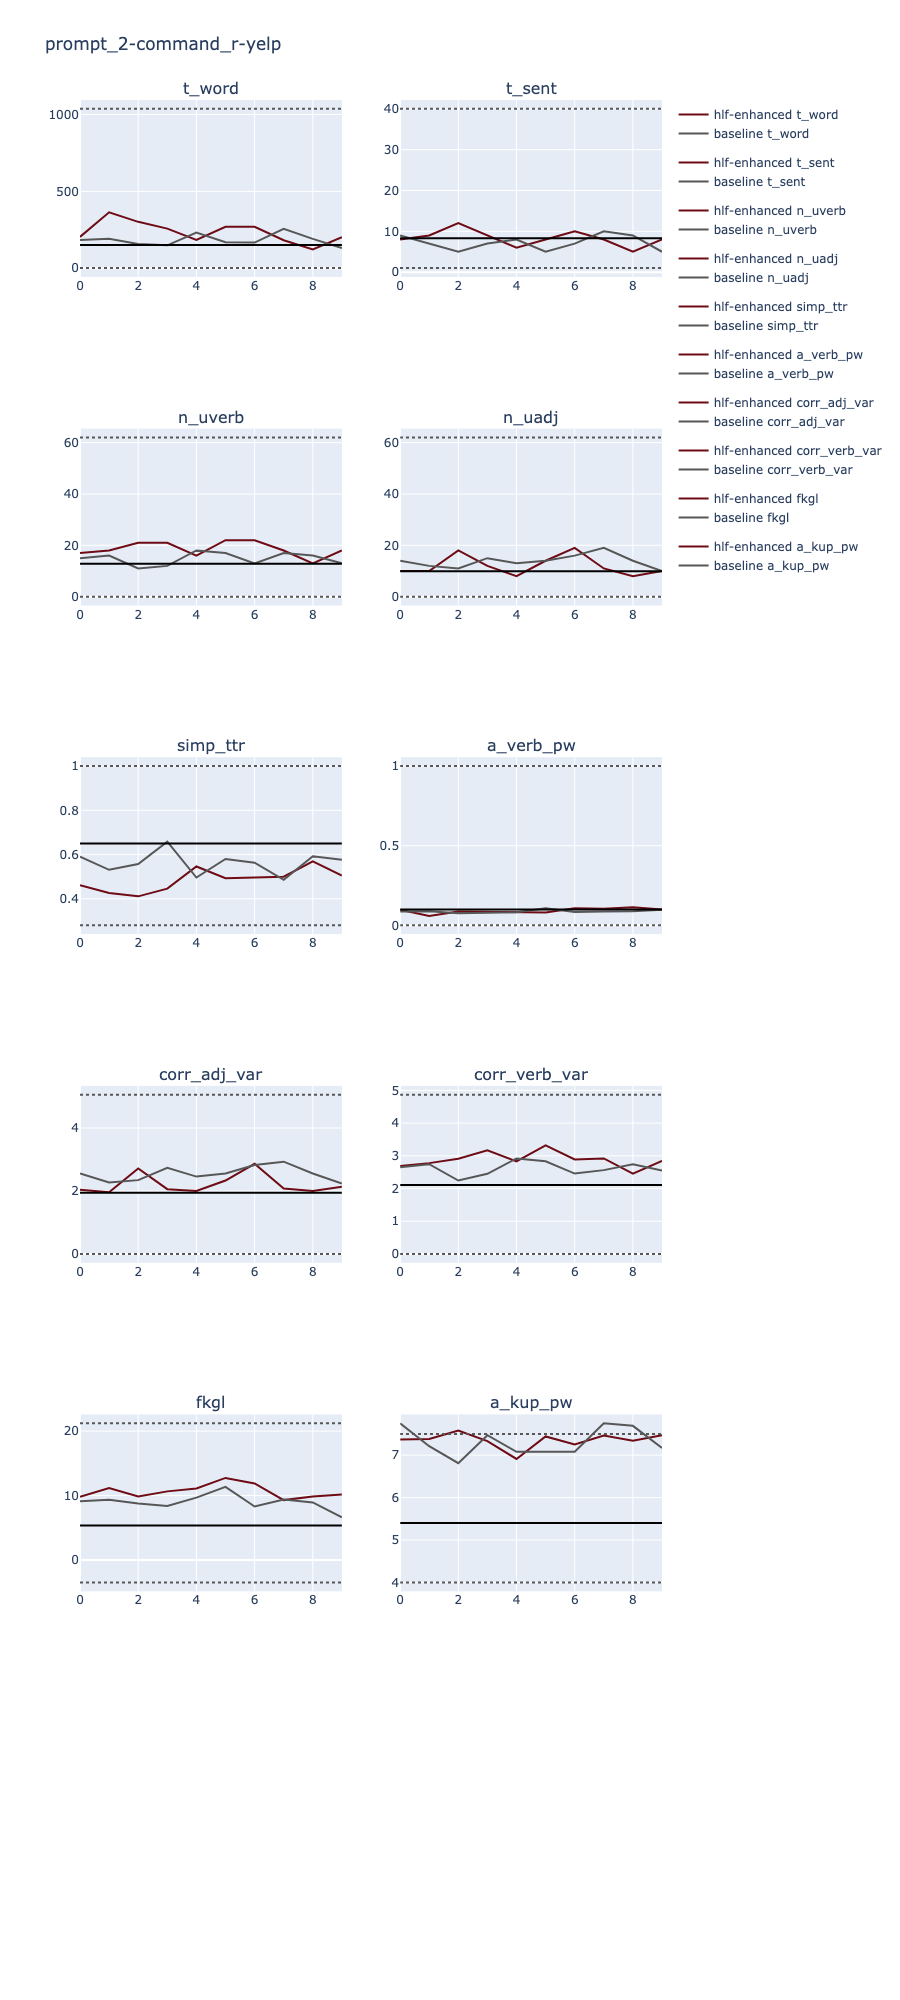
\includegraphics[width=\textwidth,height=0.9\textheight,scale=1]{plots/prompt_2/prompt_2-command_r-yelp/prompt_2-command_r-yelp.png}
    \caption{Command R on Yelp Corpus\\Prompt With Examples\\Extraneous Input}
    \label{fig:command_r-prompt2-yelp}
\end{figure*}
\begin{figure*}[ht]
    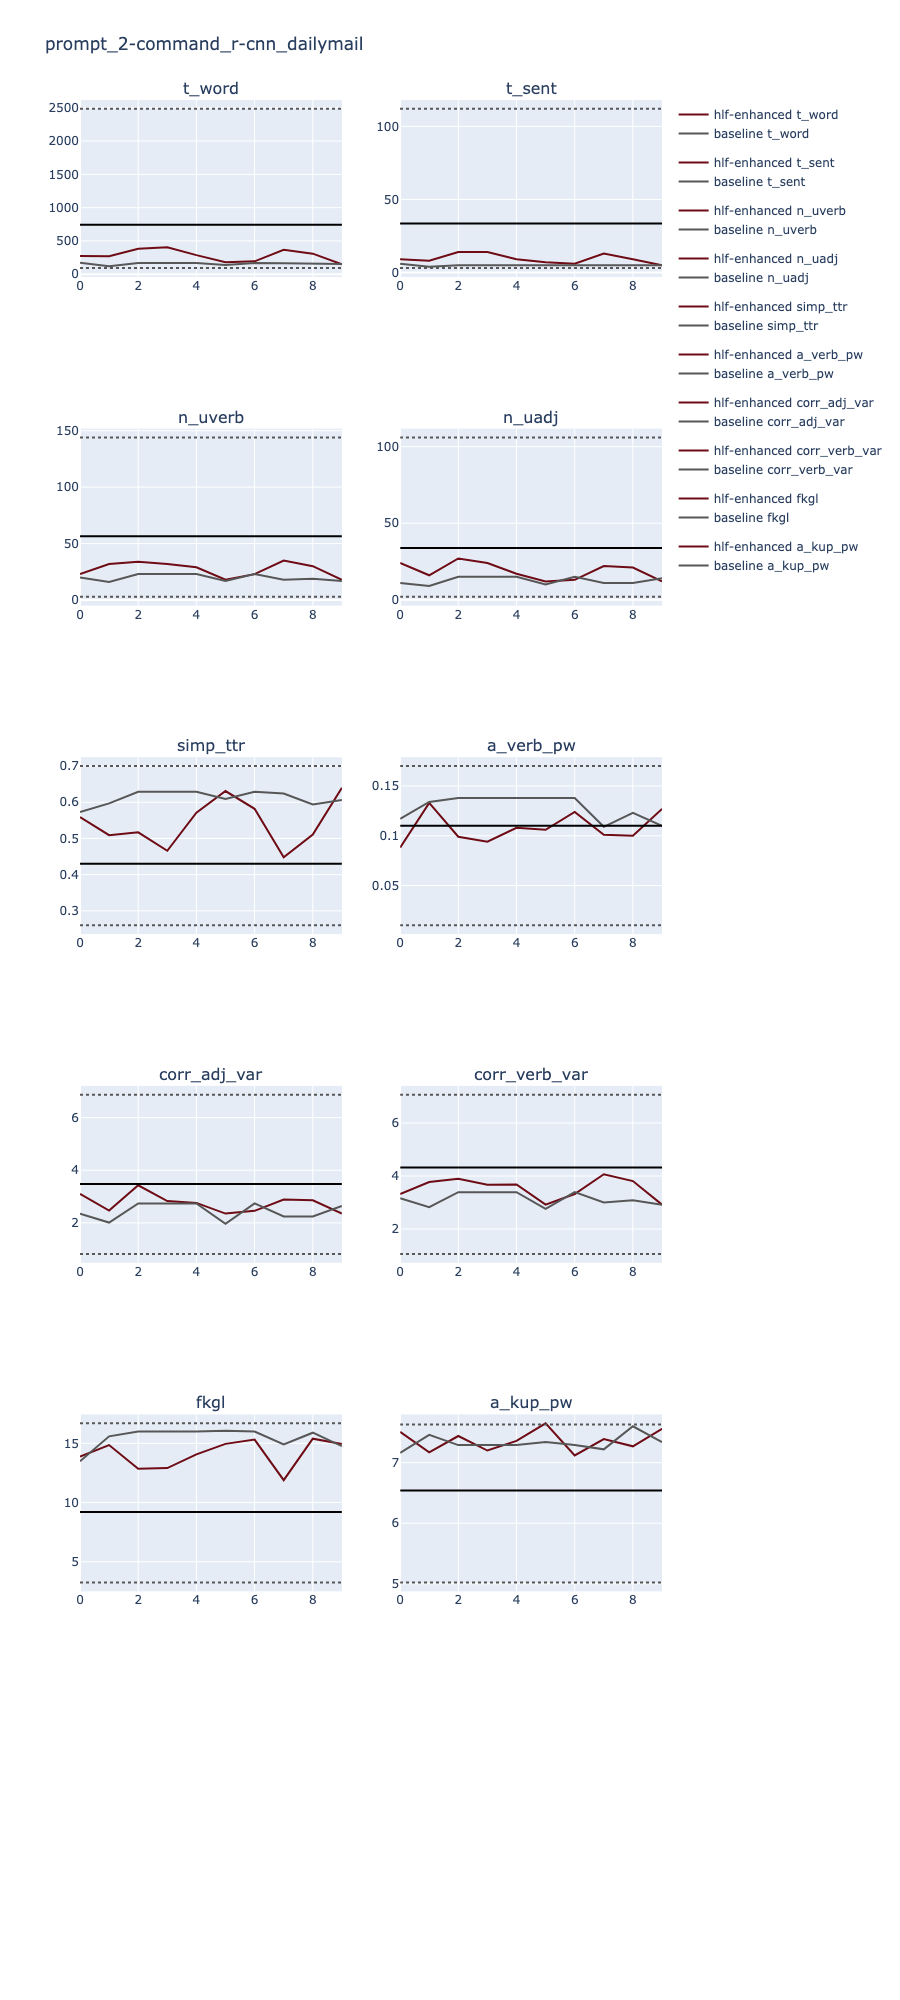
\includegraphics[width=\textwidth,height=0.9\textheight,scale=1]{plots/prompt_2_ifd/prompt_2-command_r-cnn_dailymail/prompt_2-command_r-cnn_dailymail.png}
    \caption{Command R on CNN Corpus\\Prompt With Examples\\Input from Corpus}
    \label{fig:command_r-prompt2-cnn-ifd}
\end{figure*}
\begin{figure*}[ht]
    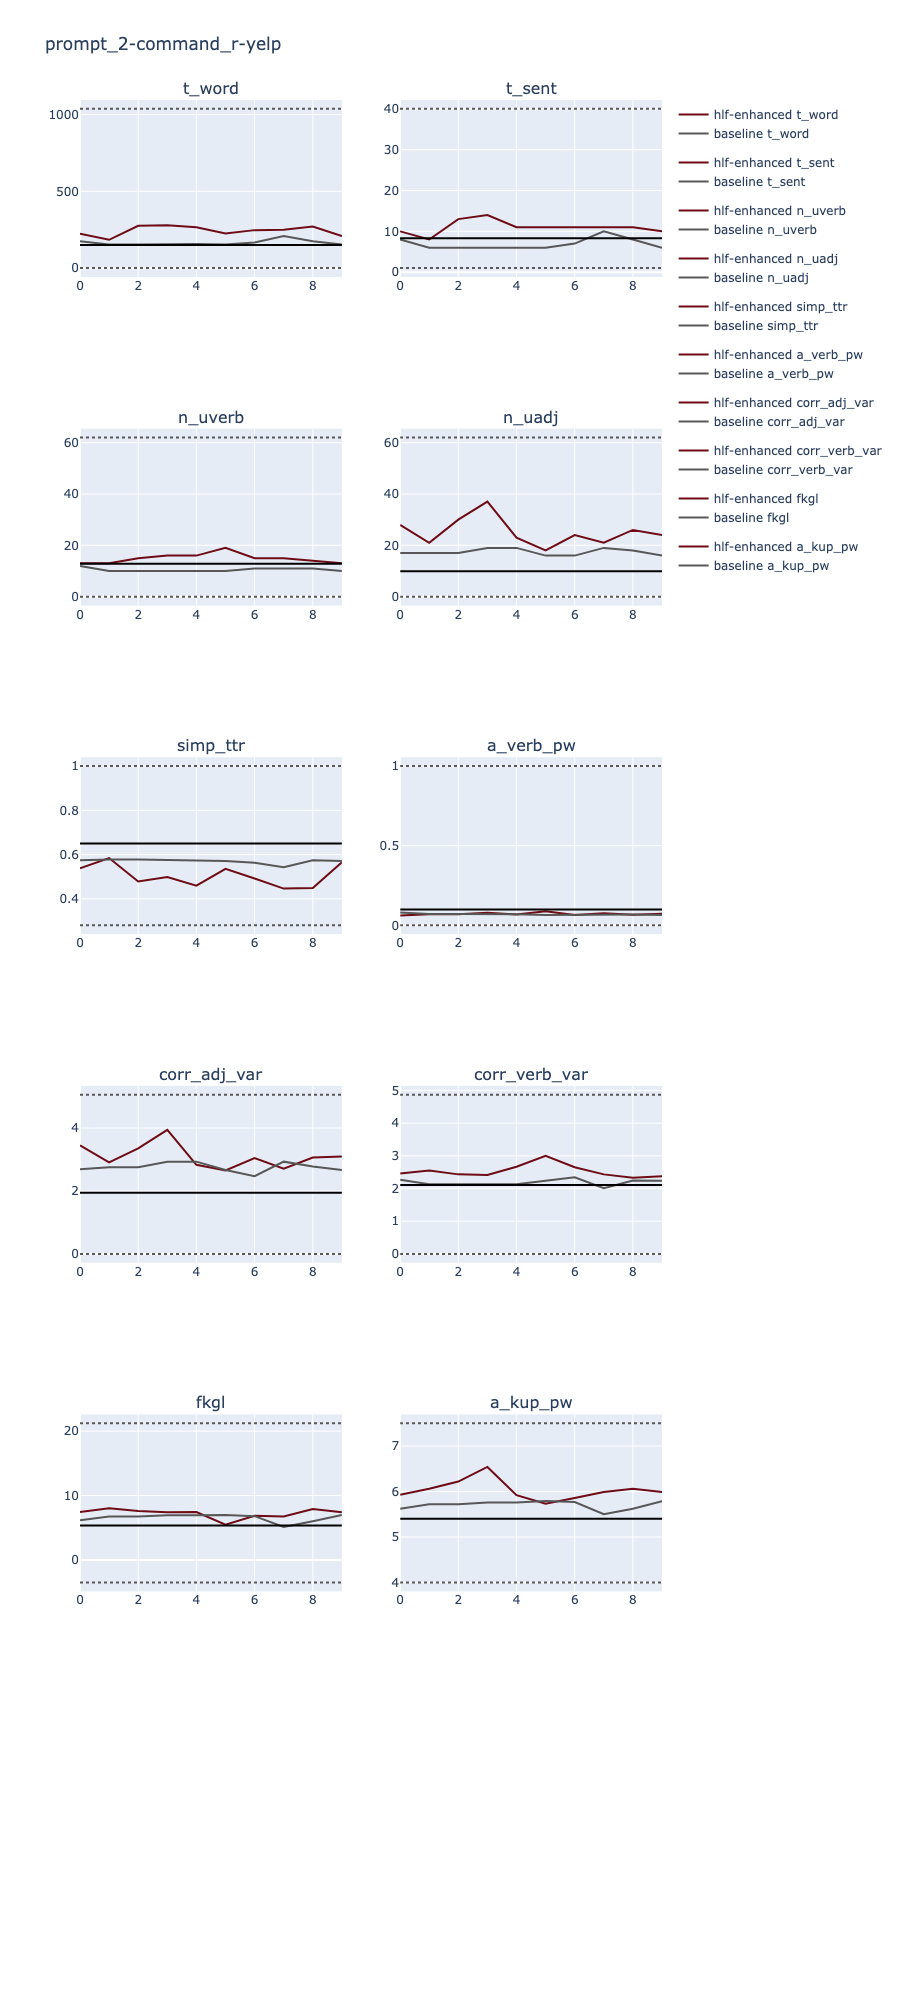
\includegraphics[width=\textwidth,height=0.9\textheight,scale=1]{plots/prompt_2_ifd/prompt_2-command_r-yelp/prompt_2-command_r-yelp.png}
    \caption{Command R on Yelp Corpus\\Prompt With Examples\\Input from Corpus}
    \label{fig:command_r-prompt2-yelp-ifd}
\end{figure*}

\end{document}